%%
%% getstart.tex -- Flight Gear documentation: The FlightGear Manual
%% Chapter file
%%
%% Copyright (C) 2002 Michael Basler
%%                  & Bernhard Buckel
%%
%% This program is free software; you can redistribute it and/or
%% modify it under the terms of the GNU General Public License as
%% published by the Free Software Foundation; either version 2 of the
%% License, or (at your option) any later version.
%%
%% This program is distributed in the hope that it will be useful, but
%% WITHOUT ANY WARRANTY; without even the implied warranty of
%% MERCHANTABILITY or FITNESS FOR A PARTICULAR PURPOSE.  See the GNU
%% General Public License for more details.
%%
%% You should have received a copy of the GNU General Public License
%% along with this program; if not, write to the Free Software
%% Foundation, Inc., 675 Mass Ave, Cambridge, MA 02139, USA.
%%
%% $Id: takeof.tex,v 0.6 2002/09/09 michael
%% (Log is kept at end of this file)

%%%%%%%%%%%%%%%%%%%%%%%%%%%%%%%%%%%%%%%%%%%%%%%%%%%%%%%%%%%%%%%%%%%%%%%%%%%%%%%%%%%%%%%%%%%%%%%
\ifchinese
\chapter{{\\}起飞:如何启动程序}
\fi
%\IfLanguageName{english}{
%\chapter{Takeoff: How to start the program}
%}{}
\IfLanguageName{french}{
\chapter{D\'{e}collage : comment d\'{e}marrer le programme}
}{}
\IfLanguageName{italian}{
\chapter{Inizio: come avviare il programma}
}{}
\label{takeoff}
%%%%%%%%%%%%%%%%%%%%%%%%%%%%%%%%%%%%%%%%%%%%%%%%%%%%%%%%%%%%%%%%%%%%%%%%%%%%%%%%%%%%%%%%%%%%%%%
\ifchinese
\markboth{\thechapter.\hspace*{1mm} 起飞}{\thesection\hspace*{1mm} 命令行参数}
\fi
%\IfLanguageName{english}{
%\markboth{\thechapter.\hspace*{1mm} TAKEOFF}{\thesection\hspace*{1mm} Command line parameters}
%}{}
\IfLanguageName{french}{
\markboth{\thechapter.\hspace*{1mm} DECOLLAGE}{\thesection\hspace*{1mm} Param\`{e}tres de ligne de commande }
}{}
\IfLanguageName{italian}{
\markboth{\thechapter.\hspace*{1mm} INIZIO}{\thesection\hspace*{1mm} Come avviare il programma }
}{}

%%%%%%%%%%%%%%%%%%%%%%%%%%%%%%%%%%%%%%%%%%%%%%%%%%%%%%%%%%%%%%%%%%%%%%%%%%%%%%%%%%%%%%%%%%%%%%%
\ifchinese
\section{环境变量}\index{环境变量}
\fi
%\IfLanguageName{english}{
%\section{Environment Variables}\index{environment variables}
%}{}
\IfLanguageName{french}{
\section{Variables d'environnement}\index{variables d'environment}
}{}
\IfLanguageName{italian}{
\section{Variabili d'ambiente}\index{Variabili d'ambiente}
}{}
%%%%%%%%%%%%%%%%%%%%%%%%%%%%%%%%%%%%%%%%%%%%%%%%%%%%%%%%%%%%%%%%%%%%%%%%%%%%%%%%%%%%%%%%%%%%%%%

\ifchinese
有两个环境变量可以在 \FlightGear{} 里定义。他们告诉 \FlightGear{} 去哪里找自己的数据和地景。

可以通过很多方式设置它们,这取决于你的系统和需求。
\fi
%\IfLanguageName{english}{
%There are two environment variables that must be defined to run \FlightGear{}.
%These tell \FlightGear{} where to find its data and scenery.
%
%You can set them in a number of ways depending on your platform and requirements.
%}{}
\IfLanguageName{french}{
Il existe deux variables d'environnement qui doivent \^{e}tre d\'{e}finies pour faire fonctionner \FlightGear{}.
Elles indiquent \`{a} \FlightGear{} o\`{u} trouver ses donn\'{e}es et ses sc\`{e}nes.

Vous pouvez les param\'{e}trer de plusieurs fa\c{c}ons en fonction de votre plate-forme et de vos besoins.
}{}

\IfLanguageName{italian}{
Ci sono due variabili d'ambiente che devono essere definite per eseguire FlightGear. Queste dicono a \FlightGear{}
dove trovare i dati e i paesaggi.
\`{e} possibile impostarle in vari modi a seconda della piattaforma e delle proprie esigienze.
}{}

\subsection{FG\_ROOT}\index{FG\_ROOT}

\ifchinese
这里放置 \FlightGear{} 将去哪里寻找数据文件,比如飞行器、导航台的位置、机场频率。在你安装 \FlightGear{} 的 \texttt{data} 子目录下。比如:\\
\texttt{/usr/local/share/FlightGear/data} 或者
\texttt{c:$\backslash$Program Files$\backslash$FlightGear$\backslash$data}.

\fi
%\IfLanguageName{english}{
%This is where \FlightGear{} will find data files such as aircraft, navigational
%beacon locations, airport frequencies. This is the \texttt{data} subdirectory
%of where you installed \FlightGear{}. e.g.
%\texttt{/usr/local/share/FlightGear/data} or
%\texttt{c:$\backslash$Program Files$\backslash$FlightGear$\backslash$data}.
%}{}
\IfLanguageName{french}{
Il s'agit de l'emplacement o\`{u} \FlightGear{} recherchera ses fichiers de donn\'{e}es comme
les a\'{e}ronefs, les emplacements des balises de navigation, les fr\'{e}quences des a\'{e}roports. Il s'agit du
sous-r\'{e}pertoire \texttt{data} de l'emplacement o\`{u} vous avez install\'{e} \FlightGear{}, par exemple :
\texttt{/usr/local/share/FlightGear/data} ou
\texttt{c:$\backslash$Program Files$\backslash$FlightGear$\backslash$data}.
}{}
\IfLanguageName{italian}{
Questa variabile indica a \FlightGear{} dove trovare i file dati come aerei, luoghi di navigazione,
e frequenze aeroportuali. Di default \`{e} una sottodirectory della cartella di installazione di
\FlightGear{}, ad esempio
\texttt{/usr/local/share/FlightGear/data} o
\texttt{c:$\backslash$Program Files$\backslash$FlightGear$\backslash$data}.
}{}

\subsection{FG\_SCENERY}\index{FG\_SCENERY}
\ifchinese
这里告诉 \FlightGear{} 去哪里找地景文件。可以在此按顺序列出要搜索的目录。在 UNIX (包括 Mac OS X)下用“:”分隔,在 Windows 下则用“;”。
\fi
%\IfLanguageName{english}{
%This is where \FlightGear{} will look for scenery files. It consists of a list
%of directories that will be searched in order. The directories are separated
%by ``:'' on Unix and ``;'' on Windows. e.g.
%}{}
\IfLanguageName{french}{
Il s'agit de l'emplacement o\`{u} \FlightGear{} recherchera ses fichiers de sc\`{e}nes. Il s'agit
d'une liste de r\'{e}pertoires qui seront analys\'{e}s de mani\`{e}re s\'{e}quentielle. Les r\'{e}pertoires
sont s\'{e}par\'{e}s par ``:'' sous Unix et ``;'' sous Windows, par exemple :
}{}
\IfLanguageName{italian}{
Questa variabile indica a FlightGear dove cercare i file degli scenari. Si compone di una lista di
directory che saranno controllate nell'ordine in cui sono scritte. Le directory sono separati da
'':'' in Unix e da '';'' su Windows, ecco due esempi:
}{}

\noindent
{\footnotesize{\texttt{/home/joebloggs/WorldScenery:/usr/local/share/FlightGear/data/Scenery}}}

\noindent
\ifchinese
或者
\fi
%\IfLanguageName{english}{
%or
%}{}
\IfLanguageName{french}{
ou
}{}
\IfLanguageName{italian}{
o
}{}

\noindent
{\footnotesize{\texttt{c:$\backslash$Program Files$\backslash$FlightGear$\backslash$data$\backslash$Scenery;c:$\backslash$Program Files$\backslash$FlightGear$\backslash$data$\backslash$WorldScenery}}}.

\ifchinese
\subsection{Windows 和 Mac OS X 下设置环境变量}
Windows 下的图形化向导和 Mac OS X 下的图形化启动器已经内部定义了这些环境变量,因此你不需要自己再去定义。然而需要从命令行启动 \FlightGear{} 时,则必须详细定义这些变量。
\fi
%\IfLanguageName{english}{
%\subsection{Environment Variables on Windows and Mac OS X}
%The graphical wizard on Windows and the GUI launcher on Mac OS X internally
%define these environment variables so you don't have to define these yourself.
%However, in case you launch \FlightGear{} from command-line, you need to
%explicitly define these variables.
%}{}
\IfLanguageName{french}{
\subsection{Variables d'environnement sous Windows et Mac OS X}
Les assistants graphiques sous Windows et le GUI launcher sous Mac OS X d\'{e}finissent
de mani\`{e}re interne ces variables d'environnement de telle sorte que vous n'avez pas besoin de les d\'{e}finir vous-m\^{e}me.
Cependant, si jamais vous lancez \FlightGear{} depuis la ligne de commande, vous devez d\'{e}finir ces variables de mani\`{e}re
explicite.
}{}

\IfLanguageName{italian}{
\subsection{Variabili di ambiente Windows e Mac OS X}
La procedura guidata su Windows e l'interfaccia grafica di avvio su Mac OS X
semplifica la vita all'utente definendo internamente queste variabili d'ambiente.
Tuttavia, nel caso in cui si avvii FlightGear da riga di comando, \`{e} necessario
definirle in modo esplicito.
}{}

%%%%%%%%%%%%%%%%%%%%%%%%%%%%%%%%%%%%%%%%%%%%%%%%%%%%%%%%%%%%%%%%%%%%%%%%%%%%%%%%%%%%%%%%%%%%%%%
\ifchinese
\section{在 UNIX/Linux 下启动模拟器}\index{启动 flightgear!Linux}\index{启动 Flightgear!Linux}
\fi
%\IfLanguageName{english}{
%\section{Launching the simulator under Unix/Linux}\index{Launching Flightgear!Linux}\index{Starting Flightgear!Linux}
%}{}
\IfLanguageName{french}{
\section{D\'{e}marrer le simulateur sous Unix/Linux}\index{D\'{e}marrer Flightgear!Linux}\index{D\'{e}marrer Flightgear!Linux}
}{}
\IfLanguageName{italian}{
\section{Avvio del simulatore in ambiente Unix / Linux}\index{Avvio del simulatore!Linux}\index{Avvio del simulatore in ambiente Unix / Linux}
}{}
%%%%%%%%%%%%%%%%%%%%%%%%%%%%%%%%%%%%%%%%%%%%%%%%%%%%%%%%%%%%%%%%%%%%%%%%%%%%%%%%%%%%%%%%%%%%%%%

\centerline{\fbox{
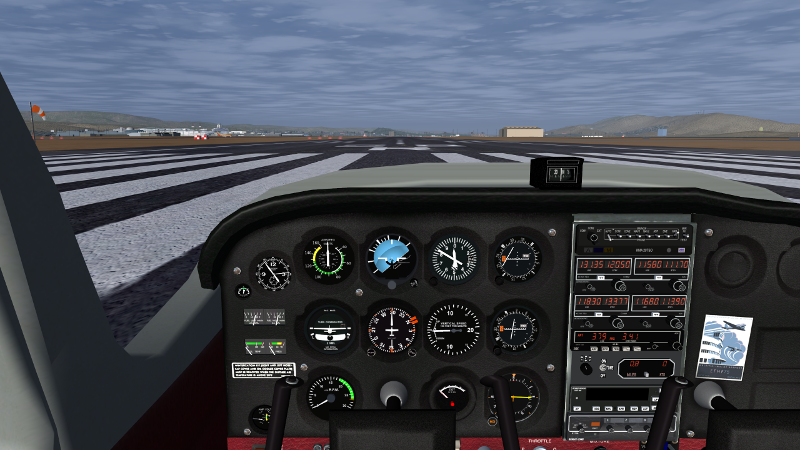
\includegraphics[clip,width=12.5cm]{img/ksfo}
}}
\smallskip
 \noindent

\ifchinese
图 3:准备起飞:\textit{在旧金山国际机场(KSFO)的默认启动点等待起飞}
\fi
%\IfLanguageName{english}{
%Fig.\,3: Ready for takeoff: \textit{Waiting at the default startup position at San Francisco Intl., KSFO.}
%}{}
\IfLanguageName{french}{
Fig.\,3 : Par\'{e} \`{a} d\'{e}coller : \textit{en attente \`{a} la position de d\'{e}marrage par d\'{e}faut de l'a\'{e}roport de San Francisco Intl., KSFO.}
}{}
\medskip
\IfLanguageName{italian}{
Fig.\,3 : Pronti al decollo: \textit{avvio predefinito a San Francisco Intl, KSFO.}
}{}
\medskip

\ifchinese
运行 \FlightGear{} 之前,你需要设置一系列环境变量:
\fi
%\IfLanguageName{english}{
%Before you can run \FlightGear{}, you need to set a couple of environment variables:
%}{}
\IfLanguageName{french}{
Avant de pouvoir d\'{e}marrer \FlightGear{}, vous devez d\'{e}finir deux variables d'environnement :
}{}
\IfLanguageName{italian}{
Prima di poter eseguire FlightGear, \`{e} necessario impostare un paio di variabili d'ambiente:
}{}


\begin{itemize}
\ifchinese
\item 你需要添加 \texttt{/usr/local/share/FlightGear/lib} 到你的 \texttt{LD\_LIBRARY\_PATH}
\item \texttt{FG\_ROOT} 必须设置为 \FlightGear{} 的数据安装目录。比如\\
\texttt{/usr/local/share/FlightGear/data}。
\item \texttt{FG\_SCENERY} 必须是一个包含地景的目录列表,用";"分隔。这个变量的功效如同系统的 \texttt{PATH} 变量。\\
比如:\texttt{\$FG\_ROOT/Scenery:\$FG\_ROOT/WorldScenery}。
\fi
%\IfLanguageName{english}{
%\item You must add \texttt{/usr/local/share/FlightGear/lib} to your \texttt{LD\_LIBRARY\_PATH}
%\item \texttt{FG\_ROOT} must be set to the data directory of your \FlightGear{} installation. e.g.% \texttt{/usr/local/share/FlightGear/data}.
%\item \texttt{FG\_SCENERY} should be a list of scenery directories, separated by '':''. This works like \texttt{PATH} when searching for scenery.
%e.g. \texttt{\$FG\_ROOT/Scenery:\$FG\_ROOT/WorldScenery}.
%}{}

\IfLanguageName{french}{
\item Vous devez ajouter \texttt{/usr/local/share/FlightGear/lib} \`{a} votre \texttt{LD\_LIBRARY\_PATH}
\item \texttt{FG\_ROOT} doit \^{e}tre param\'{e}tr\'{e} pour pointer vers le r\'{e}pertoire contenant les donn\'{e}es de votre installation de  \FlightGear{}, par exemple : \texttt{/usr/local/share/FlightGear/data}.
\item \texttt{FG\_SCENERY} doit \^{e}tre une liste de r\'{e}pertoires de sc\`{e}nes, s\'{e}par\'{e}s par '':''. Ce fonctionnement est semblable \`{a} celui de \texttt{PATH} lorsqu'on recherche des sc\`{e}nes.
par exemple : \texttt{\$FG\_ROOT/Scenery:\$FG\_ROOT/WorldScenery}.
}{}

\IfLanguageName{italian}{
\item \`{e} necessario aggiungere \texttt{/usr/local/share/FlightGear/lib} er la variabile \texttt{LD\_LIBRARY\_PATH}
\item \texttt{FG\_ROOT} ddeve essere impostata con il percorso della directory d'installazione di \FlightGear{}. (Ad esempio : \texttt{/usr/local/share/FlightGear/data}).
\item \texttt{FG\_SCENERY} deve contenere una lista di percorsi di cartelle, separati da '':''. Questa variabile indica a
FlightGear dove cercare gli scenari. (Esempio di variabile su linux: \texttt{\$FG\_ROOT/Scenery:\$FG\_ROOT/WorldScenery}).
}{}

\end{itemize}

\noindent
\ifchinese
在 Bourne shell(及兼容型)里添加这些变量:
\fi
%\IfLanguageName{english}{
%To add these in the Bourne shell (and compatibles):
%}{}
\IfLanguageName{french}{
Pour les ajouter dans le Bourne shell (et compatibles) :
}{}
\IfLanguageName{italian}{
Per aggiungere queste variabili nella Bourne shell (e compatibili):
}{}
\begin{verbatim}
LD_LIBRARY_PATH=/usr/local/share/FlightGear/lib:$LD_LIBRARY_PATH
export LD_LIBRARY_PATH
FG_HOME=/usr/local/share/FlightGear
export FG_HOME
FG_ROOT=/usr/local/share/FlightGear/data
export FG_ROOT
FG_SCENERY=$FG_ROOT/Scenery:$FG_ROOT/WorldScenery
export FG_SCENERY
\end{verbatim}
\noindent
\ifchinese
或者在 C Shell (其兼容型)
\fi
%\IfLanguageName{english}{
% or in C shell (and compatibles):
%}{}
\IfLanguageName{french}{
 ou en C shell (et compatibles) :
}{}
\IfLanguageName{italian}{
 Per aggiungere queste variabili nella C shell (e compatibili):
}{}

\begin{verbatim}
setenv LD_LIBRARY_PATH=\
  /usr/local/share/FlightGear/lib:$LD_LIBRARY_PATH
setenv FG_HOME=/usr/local/share/FlightGear
setenv FG_ROOT=/usr/local/share/FlightGear/data
setenv FG_SCENERY=\
  $FG_HOME/Scenery:$FG_ROOT/Scenery:$FG_ROOT/WorldScenery
\end{verbatim}

\ifchinese
当你设置好这些环境变量以后,只需要这样简单的启动 \FlightGear{} 
\fi
%\IfLanguageName{english}{
% Once you have these environment variables set up, simply start \FlightGear{} by running
%}{}
\IfLanguageName{french}{
 Une fois que ces variables d'environnement ont \'{e}t\'{e} param\'{e}tr\'{e}es, d\'{e}marrez tout simplement \FlightGear{} en utilisant la commande
}{}
\IfLanguageName{italian}{
 Una volta impostate queste variabili d'ambiente, \`{e} sufficiente avviare \FlightGear{} eseguendo
}{}

\medskip

\texttt{fgfs -$ $-option1 -$ $-option2\dots}
\medskip

\ifchinese
关于详细的命令行选项将会在 ~\ref{options} 小节介绍。
\fi
%\IfLanguageName{english}{
%Command-line options are described in Chapter~\ref{options}.
%}{}
\IfLanguageName{french}{
Les options de ligne de commande sont d\'{e}crites dans le chapitre~\ref{options}.
}{}
\IfLanguageName{italian}{
Le opzioni della riga di comando sono descritte nel capitolo~\ref{options}.
}{}

%%%%%%%%%%%%%%%%%%%%%%%%%%%%%%%%%%%%%%%%%%%%%%%%%%%%%%%%%%%%%%%%%%%%%%%%%%%%%%%%%%%%%%%%%%%%%%%
\ifchinese
\section{在 Windows 下启动模拟器}\index{启动 Flightgear!Windows}\index{启动 Flightgear!Windows}
\fi
%\IfLanguageName{english}{
%\section{Launching the simulator under Windows}\index{Launching Flightgear!Windows}\index{Starting Flightgear!Windows}
%}{}
\IfLanguageName{french}{
\section{D\'{e}marrer le simulateur sous Windows}\index{D\'{e}marrer Flightgear!Windows}\index{D\'{e}marrer Flightgear!Windows}
}{}
\IfLanguageName{french}{
\section{Avvio del simulatore sotto Windows}\index{Avvio del simulatore sotto Windows}\index{Avvio del simulatore!Windows}
}{}
%%%%%%%%%%%%%%%%%%%%%%%%%%%%%%%%%%%%%%%%%%%%%%%%%%%%%%%%%%%%%%%%%%%%%%%%%%%%%%%%%%%%%%%%%%%%%%%

\ifchinese
预编译好的 Windows 二进制包含一个图形化的向导可用来启动 \FlightGear{}。只需在开始菜单里双击 \texttt{FlightGear Launcher} 菜单项即可,或者双击桌面图标。启动器将会让你选择飞行器,起始机场和跑道,时间,当前天气以及大量其他选项。
\fi
%\IfLanguageName{english}{
%The pre-built windows binaries come complete with a graphical wizard to start \FlightGear{}. Simply
%double-click on the \texttt{FlightGear Launcher} Start Menu item, or the icon on the Desktop. The
%launcher allows you to select your aircraft, the start airport and runway, time of day, current weather, and lots
%of other settings.
%}{}
\IfLanguageName{french}{
Les binaires pr\'{e}-compil\'{e}s pour Windows sont livr\'{e}s avec un assistant graphique pour d\'
{e}marrer \FlightGear{}. Cliquez tout simplement sur l'\'{e}l\'{e}ment \texttt{FlightGear Launcher} du menu
D\'{e}marrer, ou double-cliquez sur l'ic\^{o}ne pr\'{e}sente sur le Bureau. L'assistant vous permet de choisir
votre a\'{e}ronef, l'a\'{e}roport de d\'{e}marrage et la piste, l'heure du jour, la m\'{e}t\'{e}o en cours, et
de nombreux autres param\`{e}tres.
}{}
\IfLanguageName{italian}{
I binari pre-costruiti per Windows sono dotati di una interfaccia grafica guidata per avviare FlightGear. \`{e}
sufficiente fare doppio clic sulla voce del menu del FlightGear Launcher nella barra di Start o sull'icona sul
desktop. Il programma di avvio consente di selezionare il vostro aereo, l'aeroporto di partenza e la pista,
l'ora del giorno, le condizioni meteo, e un sacco di altre impostazioni.}{}

 \centerline{\fbox{
\includegraphics[clip,width=12.5cm]{launcher}
}}
\smallskip
\noindent
\ifchinese
图 4:\textit{FlightGear Launcher}
\fi
%\IfLanguageName{english}{
%Fig.\,4: \textit{The FlightGear Launcher}
%}{}
\IfLanguageName{french}{
Fig.\,4: \textit{L'assistant de d\'{e}marrage de FlightGear}
}{}
\IfLanguageName{italian}{
Fig.\,4: \textit{Il launcher di FlightGear sotto Windows}
}{}

\medskip
\ifchinese
第一次运行的时候会要求设置 \texttt{FG\_ROOT} 变量(一般是 \texttt{c:$\backslash$Program Files$\backslash$FlightGear$\backslash$data})和 \texttt{FG\_SCENERY} 变量,这是你已安装地景的目录列表,一般是:

\medskip
\texttt{c:$\backslash$Program Files$\backslash$FlightGear$\backslash$data$\backslash$Scenery}.
\medskip

如果你设置的值是无效的或者后来你修改了地景的目录,你可以按“Prev”按钮到向导的第一页来修改设置。
\fi
%\IfLanguageName{english}{
%The first time your run it, you will be asked to set your \texttt{FG\_ROOT} variable
%(normally \texttt{c:$\backslash$Program Files$\backslash$FlightGear$\backslash$data}) and \texttt{FG\_SCENERY}.
%This should be a list of the directories where you have installed scenery, typically
%
%\medskip
%\texttt{c:$\backslash$Program Files$\backslash$FlightGear$\backslash$data$\backslash$Scenery}.
%\medskip
%
%If you set invalid values or change your scenery directories later, you can
%change the settings by pressing the ''Prev'' button from the first page of
%the launcher.
%}{}
\IfLanguageName{french}{
La premi\`{e}re fois que vous le lancerez, il vous sera demand\'{e} de param\'{e}trer vos variables \texttt{FG\_ROOT}
(g\'{e}n\'{e}ralement \texttt{c:$\backslash$Program Files$\backslash$FlightGear$\backslash$data}) et \texttt{FG\_SCENERY}.
Ce cette derni\`{e}re variable doit contenir une liste de r\'{e}pertoire(s) o\`{u} vous avez install\'{e} des sc\`{e}nes,
typiquement :

\medskip
\texttt{c:$\backslash$Program Files$\backslash$FlightGear$\backslash$data$\backslash$Scenery}.
\medskip

Si vous indiquez des valeurs incorrectes ou si vous modifiez les r\'{e}pertoires de vos sc\`{e}nes apr\`{e}s coup, vous pourrez
corriger ces valeurs et appuyant sur le bouton ''Pr\'{e}c\'{e}dent'' \`{a} partir de la premi\`{e}re page de l'assistant.
}{}

\IfLanguageName{italian}{
Al primo avvio, verr\`{a} chiesto di impostare la variabile \texttt{FG\_ROOT}
(generalmente  \texttt{c:$\backslash$Program Files$\backslash$FlightGear$\backslash$data}) e la variabile \texttt{FG\_SCENERY}.
Quest'ultima dovrebbe essere un elenco delle directory dove avete installato i paesaggi, solitamente

\medskip
\texttt{c:$\backslash$Program Files$\backslash$FlightGear$\backslash$data$\backslash$Scenery}.
\medskip

\`{E} possibile modificare le impostazioni successivamente premendo il tasto "Precedente" nella prima pagina del programma.
}{}

\ifchinese
\subsection{从命令行启动}
\fi
%\IfLanguageName{english}{
%\subsection{Launching from the command line}
%}{}
\IfLanguageName{french}{
\subsection{Lancement \`{a} partir de la ligne de commande}
}{}
\IfLanguageName{italian}{
\subsection{Avvio dalla riga di comando}
}{}

\ifchinese
另外,你可以从命令行启动 FlightGear。要这么做你需要手动设置 \texttt{FG\_ROOT} 和 \texttt{FG\_SCENERY} 环境变量。

打开一个命令行终端,切换到你安装的二进制目录下(一般是
\texttt{c:$\backslash$Program Files$\backslash$FlightGear$\backslash$bin$\backslash$Win32})
,键入如下命令修改环境变量
\fi
%\IfLanguageName{english}{
%Alternatively, you can run FlightGear from the command line. To do this, you
%need to set up the \texttt{FG\_ROOT} and \texttt{FG\_SCENERY} environment
%variables manually.
%
%Open a command shell, change to the directory where your binary resides
%(typically something like
%\texttt{c:$\backslash$Program Files$\backslash$FlightGear$\backslash$bin$\backslash$Win32}),
%set the environment variables by typing
%}{}
\IfLanguageName{french}{
Alternativement, vous pouvez d\'{e}marrer FlightGear \`{a} partir de la ligne de commande. Pour cela, vous devez param\'{e}trer
les variables d'environnement \texttt{FG\_ROOT} et \texttt{FG\_SCENERY} manuellement.

Ouvrez une invite de commandes, placez-vous dans le r\'{e}pertoire o\`{u} sont positionn\'{e}s vos binaires
(g\'{e}n\'{e}ralement quelque chose comme
\texttt{c:$\backslash$Program Files$\backslash$FlightGear$\backslash$bin$\backslash$Win32}),
puis param\'{e}trez les variables d'environnement en tapant :
}{}

\IfLanguageName{italian}{
In alternativa, \`{e} possibile eseguire FlightGear dalla riga di comando. Per fare questo, \`{e} necessario impostare le variabili
\texttt{FG\_ROOT} e \texttt{FG\_SCENERY} manualmente.

Aprire il prompt dei comandi, passare alla directory in cui risiedono i binari di FlightGear
(normalmente \texttt{c:$\backslash$Program Files$\backslash$FlightGear$\backslash$bin$\backslash$Win32})
E impostare le variabili d'ambiente digitando
}{}

\medskip
\begin{verbatim}
SET FG_HOME="c:\Program Files\FlightGear"
SET FG_ROOT="c:\Program Files\FlightGear\data"
SET FG_SCENERY="c:\Program Files\FlightGear\data\Scenery"
\end{verbatim}
\medskip

\noindent
\ifchinese
并调用 \FlightGear{}(在同一个命令行终端,环境设定只对当前的命令行有效),可以键入
\fi
%\IfLanguageName{english}{
% and invoke \FlightGear{} (within the same Command shell, as environment
% settings are only valid locally within the same shell) via
%}{}
\IfLanguageName{french}{
 et d\'{e}marrez \FlightGear{} (dans la m\^{e}me fen\^{e}tre d'invite de commandes, car les variables d'environnement sont valides
uniquement localement au sein de la m\^{e}me invite de commandes) par l'interm\'{e}diaire de la commande :
}{}
\IfLanguageName{italian}{
e richiamare FlightGear (all'interno dello stesso prompt dei comandi, dato che impostazioni d'ambiente sopra dichiarate
ono valide solo localmente all'interno della stessa shell) tramite
}{}
\medskip

\texttt{fgfs -$ $-option1 -$ $-option2\dots}
\medskip

\ifchinese
命令行选项在 ~\ref{options} 小节有详细介绍。当然你也可以用 Windows 文本编辑器(比如记事本)创建一个批处理文件,文件里输入上面这些命令。从最佳的性能考虑,运行 \FlightGear{} 时建议最小化文本输出窗口。
\fi
%\IfLanguageName{english}{
%Command-line options are described in Chapter~\ref{options}.
%Of course, you can create a batch file with a Windows text editor (like notepad)
%using the lines above.
%For maximum performance it is recommended that you to minimize (iconize) the
%text output window while running \FlightGear{}.
%}{}
\IfLanguageName{french}{
Les options de ligne de commande sont d\'{e}crites dans le chapitre~\ref{options}.
Naturellement, vous pouvez cr\'{e}er un fichier \textit{batch} avec un \'{e}diteur
de texte Windows (comme le bloc-notes) contenant les lignes ci-dessus.
Pour obtenir les meilleures performances \`{a} l'ex\'{e}cution, il est recommand\'{e} de
r\'{e}duire (ic\^{o}nifier) la fen\^{e}tre de sortie pendant que \FlightGear{} est en fonctionnement.
}{}
\IfLanguageName{italian}{
Le opzioni della riga di comando sono descritte nel capitolo~\ref{options}.

Naturalmente, \`{e} possibile creare un file batch con un editor di testo di Windows (come notepad)
utilizzando i comandi di cui sopra. Per le massime prestazioni si consiglia di ridurre al minimo
(Iconize) la finestra di output di testo (il prompt) durante l'esecuzione del simulatore.
}{}


%%%%%%%%%%%%%%%%%%%%%%%%%%%%%%%%%%%%%%%%%%%%%%%%%%%%%%%%%%%%%%%%%%%%%%%%%%%%%%%%%%%%%%%%%%%%%%%
\ifchinese
\section{在 Mac OS X 下启动模拟器}\index{启动 Flightgear!Mac OS X}\index{启动 Flightgear!Mac OS X}
\fi
%\IfLanguageName{english}{
%\section{Launching the simulator under Mac OS X}\index{Launching Flightgear!Mac OS X}\index{Starting Flightgear!Mac OS X}
%}{}
\IfLanguageName{french}{
\section{D\'{e}marrer le simulateur sous Mac OS X}\index{D\'{e}marrer Flightgear!Mac OS X}\index{D\'{e}marrer Flightgear!Mac OS X}
}{}
\IfLanguageName{italian}{
\section{Avvio del simulatore sotto Mac OS X}\index{Avvio del simulatore!Mac OS X}\index{Avvio del simulatore sotto Mac OS X}
}{}
%%%%%%%%%%%%%%%%%%%%%%%%%%%%%%%%%%%%%%%%%%%%%%%%%%%%%%%%%%%%%%%%%%%%%%%%%%%%%%%%%%%%%%%%%%%%%%%

\ifchinese
Mac OS X 的预编译的二进制包已经包括了一个图形化的启动器。只需要在 /Applications 文件下双击 \FlightGear{} 图标即可打开如图5所示的图形化启动器。启动器允许你:

\begin{itemize}
\item 选择一个飞行器和一个机场
\item 启用/禁用自动地景下载(使用 \TerraSync{})
\item 启用/禁用导航地图(Atlas)
\item 启动 \FlightGear{}
\end{itemize}

下面的章节将会介绍如何使用这些特性。
\fi
%\IfLanguageName{english}{
%The prebuilt binary package for Mac OS X comes with the GUI launcher. Simply double-click the \FlightGear{} icon
%on /Applications folder shows up the GUI launcher window as shown in Fig. 5. The launcher allows you to :
%
%\begin{itemize}
%\item Select an aircraft and an airport
%\item Enable/Disable automatic scenery download (using \TerraSync{})
%\item Enable/Disable the Navigation Map (Atlas)
%\item Launch \FlightGear{}
%\end{itemize}
%
%The following sections describe the use of these features.
%}{}

\IfLanguageName{french}{
Le paquetage de binaires pr\'{e}-compil\'{e}s pour Mac OS X est livr\'{e} avec un assistant en mode graphique.
Double-cliquez simplement sur l'ic\^{o}ne \FlightGear{} dans le dossier /Applications pour lancer la fen\^{e}tre
GUI launcher comme d\'{e}montr\'{e} \`{a} la Fig. 5. L'assistant vous permet :

\begin{itemize}
\item de choisir un a\'{e}ronef et un a\'{e}roport
\item d'activer/d\'{e}sactiver le t\'{e}l\'{e}chargement automatique des sc\`{e}nes (en utilisant \TerraSync{})
\item d'activer/d\'{e}sactiver la carte de navigation (Atlas)
\item de d\'{e}marrer \FlightGear{}
\end{itemize}

Les sections suivantes d\'{e}crivent l'utilisation de ces fonctionnalit\'{e}s.
}{}

\IfLanguageName{italian}{
LIl pacchetto binario precompilato per Mac OS X viene fornito con l'interfaccia di avvio guidata.
Semplicemente facendo doppio clic sull'icona di FlightGear nella cartella /Applications si dovrebbe aprire
la finestra di avvio come mostrato in Fig. 5. Il Launcher permette di:

\begin{itemize}
\item Selezionare un aereo e un aeroporto
\item Attivare/Disattivare il download automatico degli scenari (usando \TerraSync{})
\item Abilitare/Disabilitare la mappa di navigazione (Atlas)
\item Lanciare \FlightGear{}
\end{itemize}

Le sezioni seguenti descrivono l'uso di queste funzioni.
}{}
\smallskip
\centerline{\fbox{
\includegraphics[clip,width=12.5cm]{img/maclauncher}
}}
\smallskip
\noindent

\ifchinese
图 5:\textit{Mac OS X 上的图形化启动器}
\fi
%\IfLanguageName{english}{
%Fig.\,5: \textit{The GUI Launcher for Mac OS X} \label{fig:maclauncher}
%}{}
\IfLanguageName{french}{
Fig.\,5: \textit{L'assistant graphique pour Mac OS X} \label{fig:maclauncher}
}{}
\IfLanguageName{italian}{
Fig.\,5: \textit{Il Launcher per Mac OS X} \label{fig:maclauncher}
}{}

\medskip

\ifchinese
\subsection{选择一个飞行器和一个机场}
启动器窗口里,可以点开飞行器或机场名称右侧的齿轮图标来选择飞行器和机场。飞行器的缩略图也会显示在窗口里。此处选择的机场将会是你的起飞机场。\FlightGear{} 使用的是 ICAO 四字机场代码,也就是用一两个字母表示国家地区代码,再用一两个字母来表示机场代码。比如,旧金山国际机场的 ICAO 代码是 KSFO,其中字母“K”在这里表示美国,而 SFO 则表示旧金山国际机场。你可以使用 \textit{Advanced features >> Position} 或 \textit{Aircraft} 选项卡来选择一个机场或一个飞行器。
\fi
%\IfLanguageName{english}{
%\subsection{Selecting an aircraft and an airport}
%At the launcher window, you can select an aircraft and an airport by clicking gear
%buttons at the right end of the airport/aircraft name. The thumbnail image of a
%selected aircraft will show up at the image panel on the window. The airport that
%you select here will be the starting point of your flight. \FlightGear{} uses
%ICAO 4-letter airport code, which is composed with one or two prefix letters
%followed by a two or three letter airport code. For example, the ICAO code for
%San Francisco International Airport is KSFO. ``K'' in this case is the prefix
%for The United States, and SFO is the airport code for San Francisco International
%Airport. You can use \textit{Advanced features >> Position} or \textit{Aircraft}
%tab to find an airport or an aircraft.
%}{}
\IfLanguageName{french}{
\subsection{Choisir un a\'{e}ronef et un a\'{e}roport}
Dans la fen\^{e}tre de l'assistant, vous pouvez choisir un a\'{e}ronef et un
a\'{e}roport en cliquant sur les boutons situ\'{e}s \`{a} droite du nom de
l'a\'{e}roport/a\'{e}ronef. L'image miniature de l'a\'{e}ronef s\'{e}lectionn\'{e}
s'affichera dans le panneau image de la fen\^{e}tre. L'a\'{e}roport que vous
choisissez ici sera le point de d\'{e}part de votre vol. \FlightGear{} utilise
les codes a\'{e}roport \`{a} quatre lettres de l'OACI, qui se compose d'une ou
deux lettres de pr\'{e}fixe, suivies de une ou deux lettres correspondant au
code a\'{e}roport. Par exemple, le code OACI de l'a\'{e}roport international
de San Francisco est KSFO. Dans cet exemple, ``K'' est le pr\'{e}fixe pour les
Etats-Unis, et SFO est le code a\'{e}roport pour l'a\'{e}roport international
de San Francisco. Vous pouvez utiliser l'onglet \textit{Fonctionnalit\'{e}s
avanc\'{e}es >> Position} ou \textit{A\'{e}ronef} pour trouver un a\'{e}roport
ou un a\'{e}ronef.
}{}
\IfLanguageName{italian}{
\subsection{Selezione di un aereo e di un aeroporto}
Nella finestra di avvio, \`{e} possibile selezionare un aereo e un aeroporto
facendo clic sull'immagine dell'ingranaggio all'estremit\`{a} destra del
nome dell'aeroporto/aereo. L'immagine in miniatura dell'aereo selezionato
apparir\`{a} in basso sulla destra nella finestra. L'aeroporto selezionato
qui sar\`{a} il punto di partenza del volo. FlightGear usa i codici ICAO di
4 lettere per distinguere gli aeroporti, ciascun codice \`{e} composto da
una o due lettere di prefisso seguite da un codice aeroportuale di due o tre
lettere. Ad esempio, il codice ICAO per San Francisco International Airport
\`{e} KSFO. "K" in questo caso \`{e} il prefisso per gli Stati Uniti, e OFS
\`{e} il codice dell'aeroporto di San Francisco International Airport. \`{e}
possibile utilizzare le funzionalit\`{a} avanzate per trovare un aeroporto
o un aereo.
}{}

\ifchinese
\subsection{启用飞行中自动地景下载}

在启动器界面选中 \textit{Download scenery on the fly},\TerraSync{} 会让地景在你飞行时自动下载。下载的地景文件会放置在
\fi
%\IfLanguageName{english}{
%\subsection{Enabling on-the-fly scenery downloading}
%
%By checking \textit{Download scenery on the fly} at the launcher window,
%the scenery data will be downloaded while you're flying using \TerraSync{}.
%The scenery downloader will install the scenery data into \\
%}{}
\IfLanguageName{french}{
\subsection{Activer le t\'{e}l\'{e}chargement des sc\`{e}nes \`{a} la vol\'{e}e}

En activant \textit{T\'{e}l\'{e}charger les sc\`{e}nes \`{a} la vol\'{e}e} dans
la fen\^{e}tre de l'assistant, les donn\'{e}es des sc\`{e}nes seront
t\'{e}l\'{e}charg\'{e}es pendant que vous volez grace \`{a} \TerraSync{}.
L'outil de t\'{e}l\'{e}chargement des scenes installera ces donn\'{e}es dans
le r\'{e}pertoire \\
}{}
\IfLanguageName{italian}{
\subsection{Attivazione del download degli scenari in volo}
Spuntando l'opzione ''Scarica scenari durante il volo'' nella finestra di avvio,
i paesaggi verranno scaricati mentre si sta volando con TerraSync. Questi
verranno installati in \\
}{}

\noindent
\texttt{/Applications/FlightGear.app/Contents/Resouces/data/Scenery-Terrasync}.

\ifchinese
\subsection{启用导航地图(Atlas)}
Mac 版的 \FlightGear{} 包括了 Atlas,用导航地图可以帮你更加舒适的制定飞行计划。选中这个选项将会在飞行时自动启动 Atlas。你不需要给 Atlas 指定任何选项,图形化的启动器已经帮你完成了。
\fi
%\IfLanguageName{english}{
%\subsection{Enabling Navigation Map (Atlas)}
%The Mac version of \FlightGear{} includes Atlas, the navigation map that helps
%your flight plan, for your convenience. Checking this option will automatically
%launch Atlas when you start the flight. You don't have to specify any Atlas
%options. The GUI launcher will specify these for you.
%}{}
\IfLanguageName{french}{
\subsection{Activer la carte de navigation (Atlas)}
La version Mac de \FlightGear{} comprend Atlas, la carte de navigation qui vous
aide \`{a} suivre votre plan de vol, pour votre confort. L'activation de cette
option lancera automatiquement Atlas lorsque vous d\'{e}marrerez votre vol.
Vous n'avez pas besoin de sp\'{e}cifier d'options Atlas. L'assistant graphique
les pr\'{e}cisera pour vous.
}{}
\IfLanguageName{italian}{
\subsection{Attivazione della mappa di navigazione (Atlas)}
La versione Mac di FlightGear comprende Atlas, la mappa di navigazione che
aiuta il vostro piano di volo, per la vostra convenienza. Selezionando questa
opzione si avvia automaticamente Atlas quando si avvia il volo. Non \`{e}
necessario specificare ulteriori opzioni. Il Launcher le imposter\`{a}
automaticamente.
}{}
\ifchinese
\subsection{启动 FlightGear —— 模拟器}
在启动器窗口上按 \textit{Start Flight} 按钮将会启动另一个窗口——FlightGear 的主窗口。\FlightGear{} 会即刻开始载入模拟器所需要的数据。在速度较慢的机器上载入所有数据可能需要较多的时间。
\fi
%\IfLanguageName{english}{
%\subsection{Launching FlightGear - the simulator}
%Clicking \textit{Start Flight} button at the launcher window opens up another
%window - the FlightGear main window. \FlightGear{} immediately starts loading
%tons of data required for simulation. It may take a while on slower machines
%to load everything.
%}{}
\IfLanguageName{french}{
\subsection{D\'{e}marrer FlightGear - le simulateur}
Cliquer sur le bouton \textit{D\'{e}marrer le vol} dans la fen\^{e}tre de
l'assistant ouvre une nouvelle fen\^{e}tre - la fen\^{e}tre principale de
FlightGear. \FlightGear{} d\'{e}marre imm\'{e}diatement le chargement des
tonnes de donn\'{e}es n\'{e}cessaires pour la simulation. Le temps de
chargement peut \^{e}tre un peu long sur des machines lentes.
}{}
\IfLanguageName{italian}{
\subsection{Avviare FlightGear - il simulatore}
Cliccando sul pulsante \textit{Start Flight} nella finestra di avvio, si apre un'altra
finestra - quella principale di FlightGear. FlightGear inizia subito il caricamento di
tonnellate di dati necessari per la simulazione. Questa operazione pu\`{o} richiedere
anche alcuni minuti sulle macchine pi\`{u} lente.
}{}

\ifchinese
\subsection{高级选项}
你可以在启动时指定 \FlightGear{} 的很多高级特性和选项。很多在 \FlightGear{} 的主窗口菜单里是不能改动的。要启动/禁用这些特性,在启动器窗口的左下角点开三角形的按钮,将会显示高级选项的选项卡。所有选项都已经保存了,所以你不用担心重新指定。
\fi
%\IfLanguageName{english}{
%\subsection{Advanced Features}
%\FlightGear{} has many features and options that you can specify at launch time. Some of
%these are not changeable from the menu in the \FlightGear{} main window. To enable /
%disable these features, click the triangle-shaped button at the left-bottom of the
%launcher window. This displays the advanced features tabs. All settings are saved
%so you don't have to respecify them.
%}{}

\IfLanguageName{french}{
\subsection{Fonctionnalit\'{e}s avanc\'{e}es}
\FlightGear{} poss\`{e}de de nombreuses fonctionnalit\'{e}s et options que vous
pouvez sp\'{e}cifier lors du d\'{e}marrage. Quelques-unes d'entre elles ne peuvent
pas \^{e}tre modifi\'{e}es \`{a} partir du menu de la fen\^{e}tre principale de
\FlightGear{}. Pour activer/d\'{e}sactiver ces fonctionnalit\'{e}s, cliquez sur
le bouton en forme de triangle dans l'angle inf\'{e}rieur gauche de la fen\^{e}tre
de l'assistant. Ceci affiche l'onglet fonctionnalit\'{e}s avanc\'{e}es. Tous les
param\`{e}tres sont sauvegard\'{e}s de mani\`{e}re \`{a} ce que vous n'ayez pas
\`{a} les resp\'{e}cifier \`{a} chaque fois.
}{}

\IfLanguageName{italian}{
\subsection{Funzioni avanzate}
\FlightGear{} ha molte caratteristiche e opzioni che \`{e} possibile specificare
in fase di avvio.

Alcune di queste non sono modificabili dal menu nella finestra principale di FlightGear.

Per abilitare/disabilitare queste funzionalit\`{a}, fare clic sul pulsante a forma di
triangolo in basso a sinistra nella finestra di avvio. Questo mostra tutte le
funzionalit\`{a} avanzate. Tutte le impostazioni vengono salvate in modo da non
doverle specificare nuovamente.
}{}
\ifchinese
\subsubsection{General, Features, 和 Rendering 选项卡}
这些选项卡可以让你指定更多 \FlightGear{} 的选项:
\begin{itemize}
\item \textbf{Save preferences on exit(退出时保存选项):} 可以将你在 \FlightGear{} 主窗口(fgfs)的菜单项里做出的改动保存到 \\ \texttt{\$HOME/.fgfs/autosave.xml}.
\item \textbf{Control(控制):} 指定使用 \FlightGear{} 时的控制设备。有几种选择 \textit{auto, joystick, mouse, 和 keyboard},除非特意改动,否则请保持\textit{auto}。
\item \textbf{Unit(单位):} 指定在 \FlightGear{} 里使用的度量衡单位。可以选择 \textit{feet(英尺)} 和 \textit{meters(米制)}。
\item \textbf{Time of day(时段):} 指定起飞时候的时段,可以选择 \textit{real, dawn, morning, noon, afternoon, dusk, evening, 和 midnight}。
\item \textbf{Season(季节):} 指定启动 \FlightGear{} 时的季节。可以选择夏季或冬季。
\item \textbf{Sound(声音):} 禁用的话将会关断 FlightGear 的所有声音。
\item \textbf{Instrumental panel(仪表板):} 初始指定使用 2D 仪表板。你也可以在 \FlightGear{} 的菜单中启用/禁用 2D 仪表板。
\item \textbf{Random objects(随机建筑物):} 指定 \FlightGear{} 是否绘制随机建筑物。
\item \textbf{AI models(AI 模式):} 指定 \FlightGear{} 是否要处理 AI 飞行器和船只。
\item \textbf{Clock never advances(时间永不推移):} 是否允许 \FlightGear{} 里的时间推移。
\item \textbf{No fuel consumption(无燃油消耗):} 飞行器在飞行时不消耗燃油。
\item \textbf{Start in a frozen state(冻结状态启动):} 在冻结状态启动 \FlightGear{}。现在好象不起作用。
\item \textbf{Display HUD(显示 HUD):} 初始时显示 HUD,你可以在飞行时按“h”键来开关 HUD。
\item \textbf{3D HUD:} 若飞行器支持,则启动 3D HUD。
\item \textbf{Real weather fetch(获取真实天气):} 启用是否获取真实的天气 METAR。
\item \textbf{Horizon effect(地平线效果):} 启用地平线效果。
\item \textbf{Cloads(云):} 启用绘制云层。
\item \textbf{3D clouds(3D 云层):} 启用绘制 3D 云层。你需要在 \FlightGear{} 模拟器主窗口的 \textit{View >> Rendering option} 菜单项里启用 \textit{3D cloud}。
\item \textbf{Turbulence(乱流):} 指定乱流的强度。0.0 是静稳 1.0 表示暴虐。你需要指定从 0.0 到 1.0 之间的数值。
\item \textbf{Visibility(能见度):} 指定能见度,米制。如果 \FlightGear{} 在你的电脑上运行很慢,你可以指定 5000 或更少。
\item \textbf{Fullscreen mode(全屏模式):} 以全屏模式启动 \FlightGear{}。
\item \textbf{Window size(窗口尺寸):} 指定 \FlightGear{} 窗口尺寸。若启用了全屏模式,这个选项将被忽略。
\item \textbf{Sky blending(天空渲染):} 启用或禁用 \FlightGear{} 根据时间和周围环境渲染天空。不要禁用这个选项,否则 \FlightGear{} 将会崩溃。
\item \textbf{Textures(材质):} 启用或禁用跑道、建筑和地景物体的材质。禁用可以获得更好的帧速率,特别是 G4 Mac。
\item \textbf{Wireframe(线帧):} 让 \FlightGear{} 绘制线帧,这样你可以看到 \FlightGear{} 如何绘制的。请只在调式和开发的情况才启用。
\item \textbf{Fog(雾):} 指定如何绘制雾。可选 \textit{disable, fastest, nicest}。
\end{itemize}
\fi
%\IfLanguageName{english}{
%\subsubsection{General, Features, and Rendering tabs}
%These tabs let you specify some of \FlightGear{} options:
%\begin{itemize}
%\item \textbf{Save preferences on exit:} lets \FlightGear{} save preferences that you changed from the menu in the \FlightGear{} (fgfs) main window will be saved to \\ \texttt{\$HOME/.fgfs/autosave.xml}.
%\item \textbf{Control:} specifies the control device you will use in \FlightGear{}. \textit{auto, joystick, mouse, and keyboard} are available. You can leave it as \textit{auto} unless you really want to change it manually.
%\item \textbf{Unit:} specifies the unit used in \FlightGear{}. \textit{feet} and \textit{meters} are available.
%\item \textbf{Time of day:} specifies the time of day. Available options are \textit{real, dawn, morning, noon, afternoon, dusk, evening, and midnight}.
%\item \textbf{Season:} specifies the season of \FlightGear{} world. You can choose either summer or winter.
%\item \textbf{Sound:} disabling this will cut all the sound in FlightGear.
%\item \textbf{Instrumental panel:} specifies if 2D panel is drawn from the beginning. You can also enable/disable the 2D panel from \FlightGear{} menu.
%\item \textbf{Random objects:} specifies whether \FlightGear{} draws random objects or not.
%\item \textbf{AI models:} specifies whether \FlightGear{} handles AI aircraft and ships.
%\item \textbf{Clock never advances:} specifies whether the clock advances in \FlightGear{} or not.
%\item \textbf{No fuel consumption:} makes aircraft consume no fuel while it's flying.
%\item \textbf{Start in a frozen state:} starts \FlightGear{} with frozen state. it does not seem working at this moment.
%\item \textbf{Display HUD:} displays HUD at the beginning, I guess. You can turn HUD on/off by pressing 'h' while you are flying.
%\item \textbf{3D HUD:} enables 3D HUD if an selected aircraft supports it.
%\item \textbf{Real weather fetch:} enables fetching real weather condition using METAR.
%\item \textbf{Horizon effect:} enables horizon effect.
%\item \textbf{Clouds:} enables drawing clouds.
%\item \textbf{3D clouds:} enables drawing 3D clouds. You need to enable 3D clouds by checking \textit{3D cloud} from the \textit{View >> Rendering option} on the \FlightGear{} simulator window.
%\item \textbf{Turbulence:} specifies the strength of turbulence. 0.0 is calm and 1.0 is severe. You need to specify value from 0.0 through 1.0
%\item \textbf{Visibility:} specifies the visibility in meter. You can specify 5000 or less if \FlightGear{} runs slow on your machine.
%\item \textbf{Fullscreen mode:} enabling this will launch \FlightGear{} as full-screen mode.
%\item \textbf{Window size:} specifies the size of \FlightGear{} window. It will be ignored when full-screen mode is enabled.
%\item \textbf{Sky blending:} enables or disables \FlightGear{} to blend the sky depending on time and surrounding environment. DO NOT disable this option, or \FlightGear{} crashes.
%\item \textbf{Textures:} enables or disables textures on runways, buildings, and scenery objects. Disabling this will give you some more fps, effective especially on G4 Macs.
%\item \textbf{Wireframe:} lets \FlightGear{} draw wire-frames so you can see how the world of \FlightGear{} is drawn. This should be enabled only for debug / development purpose.
%\item \textbf{Fog:} specifies how fog is drawn. \textit{disable, fastest, nicest} are available.
%\end{itemize}
%}{}

\IfLanguageName{french}{
\subsubsection{Onglets G\'{e}n\'{e}ralit\'{e}s, Fonctionnalit\'{e}s et Rendu}
Ces onglets vous permettent de d\'{e}finir certaines options de \FlightGear{} :
\begin{itemize}
\item \textbf{Sauvegarder les pr\'{e}f\'{e}rences \`{a} la fermeture :} permet \`{a} \FlightGear{} de sauvegarder les pr\'{e}f\'{e}rences que vous avez modifi\'{e}es \`{a} partir du menu dans la fen\^{e}tre principale de \FlightGear{} (fgfs) vers le fichier \\ \texttt{\$HOME/.fgfs/autosave.xml}.
\item \textbf{Contr\^{o}les :} pr\'{e}cise le moyen de contr\^{o}le que vous utiliserez dans \FlightGear{}. \textit{auto, joystick, souris et clavier} sont disponibles. Vous pouvez conserver ce param\`{e}tre en mode \textit{auto} sauf si vous tenez \`{a} le param\'{e}trer manuellement.
\item \textbf{Unit\'{e}s :} d\'{e}finit l'unit\'{e} utilis\'{e}e dans \FlightGear{}. Les \textit{pieds} et les \textit{m\`{e}tres} sont disponibles.
\item \textbf{Heure du jour :} fixe l'heure du jour. Les options disponibles sont \textit{r\'{e}elle, aube, matin, midi, apr\`{e}s-midi, cr\'{e}puscule, soir et minuit}.
\item \textbf{Saison :} d\'{e}finit la saison du monde \FlightGear{}. Vous pouvez choisir \'{e}t\'{e} ou hiver.
\item \textbf{Son :} la d\'{e}sactivation de cette option coupera le son dans FlightGear.
\item \textbf{Panneaux d'instruments :} pr\'{e}cise si un panneau 2D est activ\'{e} par d\'{e}faut. Vous pouvez \'{e}galement activer/d\'{e}sactiver le panneau 2D \`{a} partir du menu \FlightGear{}.
\item \textbf{Objets al\'{e}atoires :} pr\'{e}cise si \FlightGear{} affichera des objets al\'{e}atoires ou non.
\item \textbf{Mod\`{e}les IA :} pr\'{e}cise si \FlightGear{} g\`{e}rera les a\'{e}ronefs et navires IA.
\item \textbf{L'horloge n'avance jamais :} d\'{e}finit si l'horloge avance dans \FlightGear{} ou non.
\item \textbf{Pas de consommation de carburant :} laisse l'avion ne consommer aucun carburant lorsqu'il vole.
\item \textbf{D\'{e}marrer dans un \'{e}tat fig\'{e} :} d\'{e}marre \FlightGear{} dans un \'{e}tat fig\'{e}. Cette option a l'air de ne pas fonctionner actuellement.
\item \textbf{Activer l'affichage t\^{e}te haute (HUD) :} affiche le HUD au d\'{e}marrage, je pense. Vous pouvez activer/d\'{e}sactiver le HUD en appuyant sur 'h' lorsque vous volez.
\item \textbf{HUD 3D :} active le HUD 3D si un avion s\'{e}lectionn\'{e} le prend en charge.
\item \textbf{M\'{e}t\'{e}o r\'{e}elle :} active la r\'{e}cup\'{e}ration des conditions m\'{e}t\'{e}o r\'{e}elles en utilisant les METAR.
\item \textbf{Effet de l'horizon :} active l'effet de l'horizon.
\item \textbf{Nuages :} active l'affichage des nuages.
\item \textbf{Nuages 3D :} active l'affichage des nuages 3D. Vous devrez activer les nuages 3D en activant la case \textit{Nuages 3D} dans le menu \textit{Affichage >> Options de rendu} dans la fen\^{e}tre du simulateur \FlightGear{}.
\item \textbf{Turbulence :} pr\'{e}cise la force des turbulences en vol. 0.0 est calme et 1.0 est forte. Vous devez sp\'{e}cifier une valeur allant de 0.0 \`{a} 1.0.
\item \textbf{Visibilit\'{e} :} sp\'{e}cifie la visibilit\'{e} en m\`{e}tres. Vous pouvez donner une valeur de 5 000 ou moins si \FlightGear{} tourne lentement sur votre machine.
\item \textbf{Mode plein \'{e}cran :} l'activation de ce param\`{e}tre lancera \FlightGear{} en mode plein \'{e}cran.
\item \textbf{Taille de la fen\^{e}tre :} d\'{e}finit la taille de la fen\^{e}tre \FlightGear{}. Sera ignor\'{e} si le mode plein \'{e}cran est activ\'{e}.
\item \textbf{Fondu du ciel :} active ou d\'{e}sactive le fondu du ciel dans \FlightGear{} en fonction du temps et de l'environnement proche. NE DESACTIVEZ PAS cette option, sous peine de voir \FlightGear{} dysfonctionner.
\item \textbf{Textures :} active ou d\'{e}sactive les textures sur les pistes, les immeubles et les objets des sc\`{e}nes. La d\'{e}sactivation vous donnera quelques images par seconde en plus, sp\'{e}cialement sur les Macs G4.
\item \textbf{Fil de fer :} demande \`{a} \FlightGear{} de dessiner le monde en fils de fer, de telle sorte que vous puissiez visualiser la mani\`{e}re dont le monde de \FlightGear{} est rendu. Ceci ne devrait \^{e}tre activ\'{e} que pour des besoins de d\'{e}bogage ou de d\'{e}veloppement.
\item \textbf{Brouillard :} pr\'{e}cise la mani\`{e}re dont le brouillard est rendu. \textit{d\'{e}sactiv\'{e}, plus rapide, plus beau} sont les options disponibles.
\end{itemize}
}{}

\IfLanguageName{italian}{
\subsubsection{Le sottoschede: Generale, Caratteristiche, Rendering}
Queste schede consentono di specificare alcune opzioni \FlightGear{} :
\begin{itemize}
\item \textbf{Salva preferenze all'uscita}: consente a \FlightGear{} di salvare le preferenze che sono state modificate nei men\`{u} della finestra principale del simulatore. Queste varranno salvate in \\ \texttt{\$HOME/.fgfs/autosave.xml}.
\item \textbf{Controllo}: specifica quale dispositivo di controllo si intende utilizzare in \FlightGear{}. Le opzioni disponibili sono: . \textit{Auto, Joystick, Mouse e  Tastiera} \'{E} preferibile lasciare l'opzione predefinita (Auto) a meno che non si voglia veramente cambiarla manualmente
\item \textbf{Unit\`{a}}: specifica l'unit\`{a} utilizzata in \FlightGear{}. Le opzioni disponibili sono \textit{Piedi} e \textit{Metri}.
\item \textbf{Ora del giorno}: indica l'ora del giorno nel simulatore. Le opzioni disponibili sono: \textit{Ora reale, Alba, Mattina, Mezzogiorno, Pomeriggio, Tramonto, Sera e Mezzanotte}.
\item \textbf{Stagione}: indica la stagione usata dal simulatore. \`{e} possibile scegliere tra estate o inverno.
\item \textbf{Audio}: la disattivazione di questa opzione toglier\`{a} tutto il suono in \FlightGear{}.
\item \textbf{Pannello strumentale}: specifica se attivare il pannello 2D. \`{e} comunque possibile abilitarlo/disabilitarlo durante il volo tramite il men\`{u} dellafinestra principale .
\item \textbf{Oggetti Random}: specifica se \FlightGear{} disegni oggetti casuali o meno.
\item \textbf{Modelli AL}: specifica se \FlightGear{} debba gestire aerei e navi casuali.
\item \textbf{Orologio congelato}: specifica se l'orologio debba avanzare in \FlightGear{} o meno.
\item \textbf{Carburante congelato}: se attivo l'aereo non consuma carburante in volo.
\item \textbf{Avviare in stato congelato}: inizia \FlightGear{} in pausa. Questa opzione \`{e} in fase di sviluppo e non sembra funzionare attualmente
\item \textbf{Visualizza HUD}: fa scegliere se visualizzare l'HUD fin dall'inizio del volo. \`{e} comunque possibile attivare/disattivare l'HUD durante il volo premendo il tasto ''h''.
\item \textbf{3D HUD:} abilita l'HUD tridimensionale se l'aeromobile selezionato lo supporta.
\item \textbf{Recupera le informazioni meteo reali}: abilita il recupero delle condizioni atmosferiche reali utilizzando METAR .
\item \textbf{Effetto Horizon}: abilita l'effetto orizzonte.
\item \textbf{Nuvole}: se attiva disegna nuvole casuali in cielo.
\item \textbf{Nubi 3D}: consente di disegnare nuvole 3D. Per visualizzarle \`{e} necessario abilitare anche l'opzione ''nuvole 3D'' nella scheda di Rendering.
\item \textbf{Turbolenze}: specifica la forza delle turbolenze. \`{e} necessario specificare un valore tra 0.0 (turbolenze assenti) e 1.0 (turbolenze forti)
\item \textbf{Visibilit\`{a}}: specifica la visibilit\`{a} in metri. \`{e} consigliato specificare 5000 o meno, sui computer meno potenti.
\item \textbf{Modalit\`{a} a schermo intero}: l'attivazione di questa opzione lancer\`{a} \FlightGear{} in modalit\`{a} a schermo intero.
\item \textbf{Dimensioni finestra}: specifica la dimensione della finestra di \FlightGear{}. Sar\`{a} ignorata quando la modalit\`{a} a schermo intero \`{e} attivata.
\item \textbf{Miscelazione cielo}: NON disabilitare questa opzione, o si bloccher\`{a} \FlightGear{}.
\item \textbf{Textures}: attiva o disattiva le texture su piste, edifici e oggetti degli scenari. La disattivazione di questo vi dar\`{a} qualche fps in pi\`{u}, visibile soprattutto su Mac G4.
\item \textbf{Wireframe}: permette a \FlightGear{} di disegnare wireframe in modo da poter vedere come viene disegnato il mondo di \FlightGear{}. Questo dovrebbe essere attivato solo per scopi di debug/sviluppo.
\item \textbf{Nebbia}: specifica come la nebbia viene disegnata. Le opzioni disponibile sono: \textit{nebbia disabilitata, grafica nebbia massima, grafica nebbia minima}.
\end{itemize}
}{}

\ifchinese
\subsubsection{Favorite 选项卡}
Favorite 列表提供了像浏览器书签一样的功能。若想保存当前选项,可以在 Favorite 选项卡窗口的顶部和底部按“+”按钮。添加到最爱以后,你就可以在选项卡里从一个配置切换到另一个配置,只需双击你要切换的那个选项即可。按“-”按钮(或者 Delete 键)将会删掉选中的最爱配置。
\fi
%\IfLanguageName{english}{
%\subsubsection{Favorite tab}
%Favorite list provides a means of preserving a named set of current options like a book mark of a web
%browser. To save the current set of options, press ``+'' button on the top window or at the bottom of
%the Favorite tab. Once favorites are added, You can switch from one configuration to another by
%double-clicking a row in the table view in the Favorite tab. Pressing ``-'' button (or delete key)
%on a favorite in the table view deletes the selected favorite.
%}{}
\IfLanguageName{french}{
\subsubsection{Onglet Favoris}
La liste des favoris offre un moyen de conserver un \'{e}tat nomm\'{e} des options actuelles,
\`{a} la fa\c{c}on du marque-pages d'un navigateur Internet. Pour sauvegarder l'\'{e}tat actuel
des options, appuyez sur le bouton ``+'' dans le haut de la fen\^{e}tre ou en-bas de l'onglet
Favoris. Une fois que les favoris ont \'{e}t\'{e} ajout\'{e}s, vous pouvez basculer d'une
configuration \`{a} l'autre en double-cliquant sur une ligne du tableau dans l'onglet Favoris.
L'appui sur le bouton ``-'' (ou sur la touche suppression) sur un favori dans le tableau efface
le favori s\'{e}lectionn\'{e}.
}{}
\IfLanguageName{italian}{
\subsubsection{Scheda Preferiti}
Questa scheda fornisce un comodo mezzo per salvare un set di opzioni come un segnalibro di un
browser web. Per salvare l'attuale serie di opzioni, premere il pulsante ''+'' nella scheda.
Una volta salvate le opzioni, \`{e} possibile passare da una configurazione all'altra facendo
doppio clic su una riga nella tabella ''Visualizza'' della scheda. Premendo il pulsante ''-''
 (o il tasto Canc) su un favorito all'interno della tabella, si elimina il preferito selezionato.
}{}

\ifchinese
\subsubsection{Position 选项卡}
可以通过在文本框输入关键字的方式找到机场或者航空母舰。可用的关键字是:
\fi
%\IfLanguageName{english}{
%\subsubsection{Position tab}
%You can find airports or aircraft carriers by searching with a keyword into the filter text area.
%Available keywords are:
%}{}
\IfLanguageName{french}{
\subsubsection{Onglet Position}
Vous pouvez trouver des a\'{e}roports ou des porte-avions en cherchant en utilisant une
recherche par mot-cl\'{e} dans la zone de texte filtre. Les mots-cl\'{e}s disponibles sont :
}{}
\IfLanguageName{italian}{
\subsubsection{Scheda Posizione}
\'{E} possibile trovare aeroporti o portaerei cercando tramite una parola chiave digitandola
nell'area di testo del filtro. Le parole chiave disponibili sono:}{}

\begin{itemize}
\ifchinese
\item 机场:
    \begin {itemize}
    \item 机场名字的一部分(如. international, ranch, 或 civil),
    \item 国家名字(如 Japan, USA, 或 France) 如果可用,
    \item 位置名字(比如城市、国家或者美国的洲名) 如果可用,
    \item IATA 代码(例如 SFO, LAX, HND)如果可用,
    \item ICAO 代码(例如 KSFO, KLAX, RJTT) —— 所有机场都可以。
    \end{itemize}
\item 航空母舰:
    \begin{itemize}
    \item 航母的名字(Nimitz 或 Eisenhower),
    \item “carrier”。
    \end{itemize}
}{}
\fi
%\IfLanguageName{english}{
%\item For airports:
%    \begin {itemize}
%    \item a part of airport name (e.g. international, ranch, or civil),
%    \item country name (such as Japan, USA, or France) if available,
%    \item location name (such as city or county or U.S. state abbrev. if available),
%    \item IATA code (such as SFO, LAX, HND) if available,
%    \item ICAO code (such as KSFO, KLAX, RJTT) - works on all airports.
%    \end{itemize}
%\item For aircraft carriers:
%    \begin{itemize}
%    \item carrier name (Nimitz or Eisenhower),
%    \item ``carrier''.
%    \end{itemize}
%}{}
\IfLanguageName{french}{
\item Pour les a\'{e}roports :
    \begin {itemize}
    \item une partie du nom de l'a\'{e}roport (par exemple : international, ranch, ou civil),
    \item le nom du pays (comme Japon, USA, ou France) si connu,
    \item le nom de l'emplacement (comme la ville ou le nom abbr\'{e}g\'{e} de l'\'{e}tat aux Etats-Unis),
    \item code IATA (comme SFO, LAX, HND) si disponible,
    \item code OACI (comme KSFO, KLAX, RJTT) - fonctionne pour tous les a\'{e}roports.
    \end{itemize}
\item Pour les porte-avions :
    \begin{itemize}
    \item nom du porte-avions (Nimitz ou Eisenhower),
    \item ``carrier''.
    \end{itemize}
}{}
\IfLanguageName{italian}{
\item Per gli aeroporti:
    \begin {itemize}
    \item Una parte del nome dell'aeroporto,
    \item Nome del paese in cui risiede l'aeroporto (come Giappone, Stati Uniti, o Francia),
    \item Nome del luogo, (ad esempio una citt\`{a} o una provincia),
    \item Codice IATA dell'aeroporto (come SFO, LAX, HND),
    \item Codice ICAO dell'aeroporto (come KSFO, KLAX, RJTT).
    \end{itemize}
\item Per le portaerei:
    \begin{itemize}
    \item Nome della portaerei (Nimitz o Eisenhower),
    \item ``Carrier'' o ``Portaerei''.
    \end{itemize}
}{}

\end{itemize}

\ifchinese
机场和航母如果搜索到符合关键字的将会在文本区域显示出来。上部面板的机场名称与当前选择的机场或航母名称同步。你可以在上部面板机场名称右侧点开齿轮按钮,进而打开这个选项卡。当你选好了一个机场,可用的跑道将会显示在"runway"按钮,你可以选择一个跑道或者保持“default”。
\fi
%\IfLanguageName{english}{
%Airports and carriers that match the keyword are shown at the table view below
%the filter text area. The airport name at the upper pane is synchronized with
%the currently selected airport or carrier. You can also open this tab by clicking
%the gear button at the right end of airport name on the top pane.
%When you choose an airport, available runways show up at the ``runway''
%pop-up button. You can choose a runway or leave it as ``default.''
%}{}
\IfLanguageName{french}{
Les a\'{e}roports et les porte-avions qui correspondent au mot-cl\'{e} sont
affich\'{e}s dans la vue du tableau sous la zone de texte filtre. Vous pouvez
\'{e}galement ouvrir cet onglet en cliquant sur le bouton situ\'{e} \`{a}
l'extr\'{e}mit\'{e} droite du nom de l'a\'{e}roport sur le panneau sup\'{e}rieur.
Lorsque vous choisissez un a\'{e}roport, les pistes disponibles s'affichent
dans le bouton pop-up ``piste''. Vous pouvez choisir une piste ou le laisser
sur ``d\'{e}faut.''
}{}
\IfLanguageName{italian}{
Gli aeroporti e le portaerei che corrispondono alla ricerca vengono visualizzate
in una tabella sotto l'area di testo del filtro. Quando si sceglie un aeroporto,
le piste disponibili sono visibili cliccando sul pulsante ``Piste''. \`{e}
possibile scegliere una pista o lasciare come ``default''.
}{}

\ifchinese
\subsubsection{Aircraft 选项卡}
你可以通过关键字搜索飞行器。可用的关键字如:
\fi
%\IfLanguageName{english}{
%\subsubsection{Aircraft tab}
%You can find aircraft by searching with a keyword into the filter text area. Available keywords are:
%}{}
\IfLanguageName{french}{
\subsubsection{Onglet A\'{e}ronefs}
Vous pouvez trouver les a\'{e}ronefs en cherchant avec un mot cl\'{e} dans la zone de texte filtre. Les mot-cl\'{e}s disponibles sont :
}{}
\IfLanguageName{ìtalian}{
\subsubsection{Scheda Aeroplani}
\'{E} possibile trovare aerei cercandoli tramite una parola chiave digitandola nell'area di testo del filtro. Le parole chiave disponibili sono:
}{}

\ifchinese
\begin{itemize}
\item 飞行器名称的一部分(比如 c172, zero, shinden)
\item 去掉 -set.xml 后缀的配置文件名称(比如 a6m2, p51d)
\item FDM(飞行动态模型)的名称 (比如 yasim, jsb)
\item 开发状态(例如 alpha, beta, production, development)
\end{itemize}
符合搜索关键字的飞行器将会在文字区域显示出来。上部面板的飞行器名称也会与选择的飞行器名称同步显示。你可以点开上部面板的飞行器名称右侧的齿轮图标打开这个选项卡。

如果你想从互联网上找到更多飞行器数据,在 Aircraft 选项卡的底部点“Get Aircraft”按钮。将会打开网络浏览器到 \textit{FlightGear Mac OS X} 的飞行器链接页面。你可以从中下载到你想要的飞行器,飞行器下载以后,可以打开 Others 选项卡来安装它。

如果在搜索飞行器的时候碰到了一些奇怪的行为,可以将飞行器的缓存文件删除可能会解决问题。打开\\ \texttt{/Applications/Utilities/Terminal.app} 并输入下面的命令以删除缓存文件:
\fi
%\IfLanguageName{english}{
%\begin{itemize}
%\item a part of aircraft name (e.g. c172, zero, shinden)
%\item configuration file name without -set.xml (e.g. a6m2, p51d)
%\item fdm (Flight Dynamics Model) name (e.g. yasim, jsb)
%\item status (e.g. alpha, beta, production, development)
%\end{itemize}
%A list of aircraft that match the keyword shows up at the table view below the filter text area. The aircraft name at the upper pane is synchronized with the currently selected aircraft. You can also open this tab by clicking the gear button at the right end of aircraft name on the top pane.
%
%If you want to find more aircraft data from the internet, click ``Get Aircraft'' button at the bottom of the Aircraft tab. It opens a web browser to lead you to the Aircraft Links page on \textit{FlightGear Mac OS X} web site. You can visit some links there and download an aircraft you want. Once an aircraft is downloaded, open ``Others'' tab to install it.
%
%If you encounter some weird behavior in searching aircraft, removing a cache file for aircraft database might solve your problem. Open \\ \texttt{/Applications/Utilities/Terminal.app} and type the following commands to remove the cache file:
%}{}
\IfLanguageName{french}{
\begin{itemize}
\item une partie du nom de l'a\'{e}ronef (par exemple : c172, zero, shinden)
\item le nom d'un fichier de configuration sans le -set.xml (par exemple : a6m2, p51d)
\item le nom du FDM (Mod\`{e}le de dynamique de vol) (par exemple : yasim, jsb)
\item le statut (par exemple : alpha, beta, production, d\'{e}veloppement)
\end{itemize}
Une liste des a\'{e}ronefs correspondant au mot cl\'{e} s'affichent dans la vue du tableau sous la zone de texte filtre. Le nom d'a\'{e}ronef sur le panneau sup\'{e}rieur est synchronis\'{e} avec l'a\'{e}ronef actuellement s\'{e}lectionn\'{e}. Vous pouvez \'{e}galement ouvrir cet onglet en cliquant sur le bouton situ\'{e} \`{a} l'extr\'{e}mit\'{e} droite du nom de l'avion sur le panneau sup\'{e}rieur.

Si vous voulez trouver plus d'a\'{e}ronefs \`{a} partir d'Internet, cliquez sur le boutou ``Obtenir des a\'{e}ronefs'' en bas de l'onglet A\'{e}ronefs. Ceci ouvrira un navigateur pour vous mener \`{a} la page Liens A\'{e}ronefs sur le site Internet \textit{FlightGear Mac OS X}. Vous pouvez consulter certains liens qui s'y trouvent et t\'{e}l\'{e}charger l'a\'{e}ronef que vous souhaitez. Une fois que l'a\'{e}ronef est t\'{e}l\'{e}charg\'{e}, ouvrez l'onglet ``Autres'' pour l'installer.

Si vous constatez un comportement anormal lorsque vous recherchez un a\'{e}ronef, supprimer un fichier de cache de la base de donn\'{e}es des a\'{e}ronefs peut r\'{e}soudre votre probl\`{e}me. Ouvrez \\ \texttt{/Applications/Utilities/Terminal.app} et tapez les commandes suivantes pour supprimer le fichier de cache :
}{}
\IfLanguageName{italian}{
\begin{itemize}
\item Una parte del nome dell'aeromobile (ad esempio C172, zero, Shinden)
\item Nome del file di configurazione senza -set.xml (per esempio A6M2, P51D)
\item Fdm (Flight Dynamics Model), ad esempio Yasim o JSB
\item Stato (ad esempio Alfa, Beta, Produzione, Sviluppo)
\end{itemize}
UL'elenco degli aeromobili corrispondenti alla ricerca verr\`{a} visualizzato in
una tabella sotto l'area di testo del filtro. Selezionando un aereo dall'elenco si
seleziona anche l'aereo da usare durante la simulazione.

Se si desidera scaricare aeromobili aggiuntivi da Internet, fare clic sul pulsante
''Get Aircraft'' (in italiano: ''Ottieni altri aerei'') nella parte inferiore della
scheda. Cos\`{i} facendo, si aprir\`{a} un browser web in una nuova finestra per
condurvi alla pagina per scaricare aerei sul sito web di FlightGear Mac OS X. Per
scaricare l'aereo desiderato cliccare sul link ''Download'' presente sotto l'immagine
dell'aereo stesso. Una volta che un aeromobile viene scaricato, \`{e} possibile
installarlo tramite la scheda ''Altro''.

Se doveste notare qualche strano comportamento durante la ricerca di un aereo,
la rimozione del file di cache del database degli aerei potrebbe risolvere il
vostro problema. Per far ci\`{o}, aprire \texttt{/Applications/Utilities/Terminal.app}
e digitare il seguente comando:
}{}

\begin{verbatim}
  cd /Applications/FlightGear.app/Contents/Resources
  rm AircraftCache.rb
\end{verbatim}

\medskip
\ifchinese
你不能从挂载硬盘的镜像文件启动 \FlightGear{},因为挂载硬盘的镜像文件是只读的,这会阻止你安装任何插件。你需要从挂载的镜像文件拷贝 \FlightGear{} 图标到安装 \texttt{/Applications} 文件夹来安装 \FlightGear{}。
\fi
%\IfLanguageName{english}{
%Note that you must not launch \FlightGear{} from mounted disk image of a prebuilt binary package since the folder in the mounted disk image is read-only, which prevents you from installing any add-on data. Vou need to install \FlightGear{} by copying the \FlightGear{} icon from the mounted disk image to \texttt{/Applications} folder.
%}{}
\IfLanguageName{french}{
Notez que vous ne devez pas lancer \FlightGear{} \`{a} partir de l'image disque d'un paquetage binaire pr\'{e}compil\'{e} car le r\'{e}pertoire de l'image disque mont\'{e}e est en lecture seule, ce qui vous emp\^{e}che d'installer toute donn\'{e}e ajout\'{e}e. Vous devez installer \FlightGear{} en copiant l'ic\^{o}ne \FlightGear{} depuis l'image disque mont\'{e}e vers le r\'{e}pertoire \texttt{/Applications}.
}{}

\ifchinese
\subsubsection{Network 选项卡}
此选项卡包括了 \FlightGear{} 的两个网络特性。一个是多用户模式,另一个是 FGCOM(一个 ATC 语音程序)。要想启用多用户模式,指定如下:
\begin{itemize}
\item \textbf{Enable Multiplay(启用多人游戏):}启用或禁用多用户模式。启用将会打开一个新的浏览器窗口来显示多人游戏服务器上的地图。
\item \textbf{Callsign(呼号):}指定地图上显示的名字。用户名必须只包括英文字母、数字、下划线和点号。当你指定的呼号使用无效字符时,\FlightGear{} 会自动退出。用户如果使用了超过 8 位字符,将只取用前 7 位。
\item \textbf{Server(服务器):}指定连接的服务器,写此文档时 \texttt{mpserver02.flightgear.org} 是可用的。
\item \textbf{Your Mac:}指定你的 Mac 的 IP 地址。一般启动器会自动探测。如果连接错误,请清空这个文本区域。
\item \textbf{Port(端口):}必须是 5000
\end{itemize}

FGCOM 让你可以像真实的 ATC 一样使用无线电设置进行语音交流。你可以按空格键用选择的无线电频率(COM1)通话。如果其他人也在用同一频率且在同一范围内,你能听到此频率中其他人的通话。FGCOM 选项包括:

\begin{itemize}
\item \textbf{Enable FGCOM in Multi Player mode:}多人游戏模式启动时打开 FGCOM。
\item \textbf{FGCOM Server:}指定 VOIP 服务器。
\end{itemize}

有关 FGCOM 和多人游戏的更多信息,请参考第 \ref{features} 章。
\fi
%\IfLanguageName{english}{
%\subsubsection{Network tab}
%This tab contains two network features of \FlightGear{}. One is multi-player mode and another is FGCOM (a voice ATC). To enable multi-player mode, specify the followings:
%\begin{itemize}
%\item \textbf{Enable Multiplay:} enables or disables multi-player mode. Enabling this will open a new browser window to show the map on a multi player server.
%\item \textbf{Callsign:} specifies the name shown in the map. Username must contain only alphabet letters, numbers, underscores, and dots. \FlightGear{} will exit when you specify a call sign with invalid characters. A user name with 8 or more characters will be truncated into the first 7 characters.
%\item \textbf{Server:} specifies the server to connect. \texttt{mpserver02.flightgear.org} is available at the time of writing this.
%\item \textbf{Your Mac:} specifies your Mac's IP address. Usually the launcher detects the address automatically. If something is wrong with network connection, clear this text field.
%\item \textbf{Port:} must be 5000
%\end{itemize}
%
%FGCOM enables you to make a real voice communication using radio setting. You can talk at a selected radio frequency (COM1) while pressing space bar. You can listen to some other player's talking in the frequency if some others are using the same frequency and you are in range. The options available for FGCOM are listed below:
%
%\begin{itemize}
%\item \textbf{Enable FGCOM in Multi Player mode:} specifies if you use FGCOM when Multiplay is enabled.
%\item \textbf{FGCOM Server:} specifies a VOIP server.
%\end{itemize}
%
%For further instructions on FGCOM, and Multiplay, please see Chapter \ref{features}.
%}{}

\IfLanguageName{french}{
\subsubsection{Onglet r\'{e}seau}
Cet onglet contient deux fonctionnalit\'{e}s r\'{e}seau de \FlightGear{}. L'une est
le mode multijoueurs et l'autre est FGCOM (un syst\`{e}me de contr\^{o}le a\'{e}rien vocal).
Pour activer le mode multijoueurs, pr\'{e}cisez les items suivants :
\begin{itemize}
\item \textbf{Activer le mode multijoueurs :} active ou d\'{e}sactive le mode multijoueurs. L'activation ouvrira une nouvelle fen\^{e}tre du navigateur pour afficher la carte sur un serveur multijoueurs.
\item \textbf{Indicatif :} pr\'{e}cise le nom affich\'{e} sur la carte. Un nom d'utilisateur peut contenir des lettres de l'alphabet, des nombres, des tirets-bas (\textit{underscores}) et des points. \FlightGear{} se terminera si vous pr\'{e}cisez un indicatif avec des caract\`{e}res invalides. Un nom d'utilisateur contenant 8 caract\`{e}res ou plus sera tronqu\'{e} avec les seuls 7 premiers caract\`{e}res.
\item \textbf{Serveur :} pr\'{e}cise le serveur auquel se connecter. \texttt{mpserver02.flightgear.org} est disponible \`{a} l'heure de l'\'{e}criture de ce document.
\item \textbf{Votre Mac :} d\'{e}finit l'adresse IP de votre Mac. G\'{e}n\'{e}ralement, l'assistant d\'{e}tecte l'adresse de mani\`{e}re automatique. Si quelque chose n'est pas exact avec votre connection r\'{e}seau, effacez le contenu de ce champ texte.
\item \textbf{Port :} doit \^{e}tre \'{e}gal \`{a} 5000.
\end{itemize}

FGCOM vous permet d'effectuer une v\'{e}ritable communication audio en utilisant
des param\`{e}tres radio. Vous pouvez parler sur une fr\'{e}quence radio
pr\'{e}cise (COM1) en appuyant sur la barre d'espace. Vous pouvez \'{e}coutez
d'autres joueurs parlant sur la fr\'{e}quence si d'autres joueurs sont sur cette
fr\'{e}quence et que vous \^{e}tes \`{a} leur port\'{e}e. Les options pour FGCOM
sont list\'{e}es ci-dessous :

\begin{itemize}
\item \textbf{Active FGCOM en mode multijoueurs :} indique si vous utilisez FGCOM lorsque le mode multijoueurs est activ\'{e}.
\item \textbf{Serveur FGCOM :} pr\'{e}cise un serveur VOIP.
\end{itemize}

Des informations compl\'{e}mentaires concernant FGCOM et le mode multijoueurs sont disponibles au chapitre \ref{features}.
}{}

\IfLanguageName{italian}{
\subsubsection{Scheda di rete (Network)}

Questa scheda contiene le impostazioni di due funzioni di rete di FlightGear.
Una \`{e} la modalit\`{a} multigiocatore e l'altra \`{e} FGCOM (un programma
che gestisce le voci del simulatore). Per attivare la modalit\`{a} multiplayer,
specificare i seguenti dati:


\begin{itemize}
\item \textbf{Abilita Multigiocatore}: attiva o disattiva la modalit\`{a} multiplayer. L'attivazione di questa opzione aprir\`{a} una nuova finestra del browser per visualizzare la mappa su un server multigiocatore.
\item \textbf{Calsign}: contiene il proprio username che verr\`{a} visualizzato dagli altri utenti e indicato sulla mappa. Pu\`{o} contenere solo lettere dell'alfabeto, numeri, caratteri di sottolineatura e punti. Un nome utente con 8 o pi\`{u} caratteri verr\`{a} troncato nei primi 7 caratteri.
\item \textbf{Server}: specifica il server a cui connettersi. mpserver02.flightgear.org \`{e} il server principale consigliato al momento della stesura di questo manuale.
\item \textbf{Your Mac} : specifica l'indirizzo IP del vostro Mac. Di solito il programma di avvio rileva automaticamente l'indirizzo; tuttavia, se ci\`{o} non dovesse accadere, \`{e} possibile impostarlo manualmente tramite questo campo.
\item \textbf{Porta}: deve essere 5000.
\end{itemize}

FGCOM consente di effettuare una vera e propria comunicazione vocale utilizzando le frequenze radio.

Si pu\`{o} parlare a una frequenza radio selezionata (COM1) premendo la barra spaziatrice.
\`{E} possibile inoltre ascoltare gli altri giocatori connessi alla stessa frequenza.
Le opzioni disponibili per FGCOM sono elencate di seguito:

\begin{itemize}
\item \textbf{FGCOM attivo in modalit\`{a} multiplayer}: specifica se utilizzare FGCOM quando il multigiocatore \`{e} abilitato.
\item \textbf{FGCOM Server}: specifica un server VOIP.
\end{itemize}

Per ulteriori istruzioni su FGCOM, e sulle impostazioni multiplayer, consultare il Capitolo \ref{features}.
}{}

\ifchinese
\subsubsection{Others 选项卡}
你可以指定除了飞行器、机场之外的任何选项。如图 11那样输入以空格隔开的选项将会传给 \FlightGear{}。你可以点开“View Options”查看所有可用的选项,有些选项可能会导致 \FlightGear{} 崩溃。如果你因为启动了这些选项导致崩溃,请告诉我们。

要想安装额外的飞行器和地景,按"Install Add-on Data."你可以指定多个文件和/或文件夹来安装到 \FlightGear{} 的数据文件夹。可用的文件类型有:
\begin{itemize}
\item zip
\item tar
\item tar.gz
\item tar.bz2
\item folder
\item 7zip (如果 7zip 已经安装)
\end{itemize}

安装成功以后可以看到一条消息提示,否则错误也会显示出来。你可以同时选择飞行器和地景,如果你选择的文件并不包括飞行器文件的话,文件也会解压缩到数据文件夹,但会被忽略。安装完新的飞行器以后,你可以到``Aircraft''选项卡里打开。
\fi
%\IfLanguageName{english}{
%\subsubsection{Others tab}
%You can specify any options other than aircraft, airport, and the options shown in the launcher. Entering space-separated options as shown in Figure 11 will pass additional options to \FlightGear{}. You can see all available options by pressing ``View Options.'' Some options might cause \FlightGear{} crash. If you encounter such crashes with a specific option, please let us know.
%
%To install additional aircraft and scenery data, press "Install Add-on Data." You can specify multiple files and/or folders to install to the \FlightGear{} data folder. Acceptable file types are:
%\begin{itemize}
%\item zip
%\item tar
%\item tar.gz
%\item tar.bz2
%\item folder
%\item 7zip (only if 7zip is installed)
%\end{itemize}
%
%You will see the message window when all the data is successfully installed, otherwise error message will show up. You can select both aircraft and scenery data at the same time. If you select an archived file that does not contain aircraft files, it will be extracted into the data folder, but will be ignored. When you finish installing new aircraft, you can select the aircraft on the ``Aircraft'' tab.
%}{}
\IfLanguageName{french}{
\subsubsection{Onglet Autres}
Vous pouvez pr\'{e}ciser toutes les options autres que a\'{e}ronef, a\'{e}roport et les options affich\'{e}es dans l'assistant. En entrant des options s\'{e}par\'{e}es par des espaces comme pr\'{e}sent\'{e} \`{a} la Figure 11, vous passerez des options additionnelles \`{a} \FlightGear{}. Vous pouvez voir toutes les options disponibles en appuyant sur ``Voir Options.'' Certaines options peuvent faire dysfonctionner \FlightGear{}. Si vous rencontrez de tels dysfonctionnements avec une option particuli\`{e}re, merci de nous le signaler.

Pour installer des a\'{e}ronefs et des sc\`{e}nes additionnelles, appuyez sur "Installer des donn\'{e}es additionnelles." Vous pouvez pr\'{e}ciser les fichiers ou r\'{e}pertoires multiples \`{a} installer dans le r\'{e}pertoire des donn\'{e}es \FlightGear{}. Les types de fichiers accept\'{e}s sont :
\begin{itemize}
\item zip
\item tar
\item tar.gz
\item tar.bz2
\item dossier
\item 7zip (seulement si 7zip est install\'{e})
\end{itemize}

Vous verrez la fen\^{e}tre d'information lorsque toutes les donn\'{e}es ont \'{e}t\'{e} correctement install\'{e}es, dans le cas contraire les messages d'erreurs y seront affich\'{e}s. Vous pouvez choisir des donn\'{e}es d'a\'{e}ronefs et de sc\`{e}nes en m\^{e}me temps. Si vous choisissez un fichier archiv\'{e} qui ne contient pas de fichiers d'a\'{e}ronefs, il sera extrait dans le r\'{e}pertoire des donn\'{e}es, mais sera ignor\'{e}. Lorsque vous aurez termin\'{e} l'installation d'un nouvel a\'{e}ronef, vous pouvez choisir l'a\'{e}ronef concern\'{e} dans l'onglet ``A\'{e}ronefs''.
}{}

\IfLanguageName{italian}{
\subsubsection{Scheda Altro}

In questa scheda \`{e} possibile specificare opzioni aggiuntive diverse dagli aerei,
aeroporti e impostazioni del programma di avvio. \'{E} possibile vedere tutte le opzioni
disponibili premendo il tasto ''Vedi opzioni''. Alcune opzioni potrebbero causare un
crash di FlightGear. Se ci\`{o} dovesse accadere con una specifica opzione, fatecelo sapere.

Sempre attraverso questa scheda, \`{e} possibile installare velivoli e scenari premendo
il tasto ''Installa dati''. \`{e} possibile specificare pi\`{u} file e/o cartelle
contenenti i dati da installare.

I tipi di file accettati sono:
\begin{itemize}
\item zip
\item tar
\item tar.gz
\item tar.bz2
\item dossier
\item 7zip (seulement si 7zip est install\'{e})
\end{itemize}

\'{E} possibile installare pi\`{u} aerei e scenari contemporaneamente. Se si seleziona un
archivio compresso che non contiene file di aeromobili, verr\`{a} estratto nella
cartella dati di FlightGear, ma verr\`{a} ignorato. Una volta terminata
l'installazione dei nuovi aeromobili, \`{e} possibile utilizzarli subito
selezionandoli nella scheda ''Aeroplani''.
}{}

\ifchinese
\subsection{从命令行启动}
你也可以在 Mac OS X 的命令行里启动模拟器。打开 Terminal.app(在 \texttt{/Applications/Utilities})并输入如下的命令:
\fi
%\IfLanguageName{english}{
%\subsection{Launching from the command line}
%You can also launch the simulator from the command line on Mac OS X. To do so, open Terminal.app (located at \texttt{/Applications/Utilities}) and type the following commands:
%}{}
\IfLanguageName{french}{
\subsection{D\'{e}marrage \`{a} partir de la ligne de commande}
Vous pouvez \'{e}galement d\'{e}marrer le simulateur \`{a} partir de la ligne de commande sur Mac OS X. Pour le faire, ouvrez Terminal.app (situ\'{e} dans \texttt{/Applications/Utilitaires}) et tapez les commandes suivantes :
}{}

\IfLanguageName{italian}{
\subsection{Avvio dalla riga di comando}
Su Mac OS X \`{e} anche possibile avviare il simulatore dalla riga di comando.
Per farlo, aprire Terminal.app (si trova in \texttt{/Applications/Utilities})
e digitare i seguenti comandi:
}{}

\begin{verbatim}
  cd /Applications/FlightGear.app/Contents/Resources
  ./fgfs --option1 --option2 ....
\end{verbatim}

\ifchinese
可以通过查看 \ref{options} 小节获取具体的命令行选项。不像其他平台,若你使用预编译的二进制包,你不需要手动指定 FG\_ROOT 和 FG\_SCENERY 这样的环境变量。
\fi
%\IfLanguageName{english}{
%See chapter \ref{options} for detail information on command line options. Unlike the other platforms, you don't have to manually specify the environment variables such as FG\_ROOT and FG\_SCENERY as long as you use a prebuilt binary package.
%}{}
\IfLanguageName{french}{
Reportez-vous au chapitre \ref{options} pour obtenir plus d'informations d\'{e}taill\'{e}es sur les options en ligne de commande. Contrairement aux autres plate-formes, vous n'avez pas besoin de pr\'{e}ciser manuellement les variables d'environnement comme FG\_ROOT et FG\_SCENERY tant que vous utilisez un paquetage binaire pr\'{e}compil\'{e}.
}{}

\IfLanguageName{italian}{
Vedere il capitolo \ref{options} per informazioni dettagliate sulle opzioni della riga di comando.
A differenza delle altre piattaforme, non \`{e} necessario specificare manualmente le
variabili di ambiente come FG\_ROOT e FG\_SCENERY se si utilizza un pacchetto binario precompilato.
}{}

%%%%%%%%%%%%%%%%%%%%%%%%%%%%%%%%%%%%%%
%%%%% Currently the following section is only available in English and Italian.  So non-italian
%%%%% versions use the English version
%%%%%%%%%%%%%%%%%%%%%%%%%%%%%%%%%%%%%%%%%%%%%%%%%%%%%%%


\IfLanguageName{italian}{
  %%%%%%%%%%%%%%%%%%%%%%%%%%%%%%%%%%%%%%%%%%%%%%%%%%%%%%%%%%%%%%%%%%%%%%%%%%%%%%%%%%%%%%%%%%%%%%%
  \section{Parametri della riga di comando\label{options}}\index{Parametri della riga di comando}
  %%%%%%%%%%%%%%%%%%%%%%%%%%%%%%%%%%%%%%%%%%%%%%%%%%%%%%%%%%%%%%%%%%%%%%%%%%%%%%%%%%%%%%%%%%%%%%%
  Di seguito \`{e} riportato un elenco completo e una breve descrizione delle numerose
  opzioni della riga di comando disponibili per FlightGear. La maggior parte di queste
  opzioni \`{e} impostabile anche attraverso i binari precompilati di FlightGear.
  Se si dispone di opzioni che si utilizzano spesso, \`{e} possibile creare un file di
  preferenze contenente una serie di opzioni della riga di comando che verranno impostate
  automaticamente. \`{e} possibile creare il file con qualsiasi editor di testo
  (per esempio: blocco note, emacs, vi).

  \begin{itemize}
  \item Sui sistemi Unix (incluso Mac OS X), scrivere le opzioni della riga di comando in
  un file con estensione \texttt{.fgfsrc}\index{.fgfsrc} posizionato nella cartella d'installazione
  del simulatore.

  \item In Windows, mettere le opzioni della riga di comando in un file chiamato
  \texttt{system.fgfsrc}
  \index{system.fgfsrc} posizionato nella directory \texttt{FG\_ROOT}
  (ad esempio, \texttt{c:$\backslash$Program Files$\backslash$FlightGear$\backslash$data}).
  \end{itemize}

}

%%%%%%%%%%% CHINESE VERSION %%%%%%%%%
\ifchinese
{
  \section{命令行参数\label{options}}\index{命令行选项}
 下面是对 \FlightGear{} 中可用的\Index{命令行选项}的完整列表和简述。大多数选项可以通过 Windows 二进制安装包提供的 \FlightGear{} 启动器来设置。

 如果你想连续多次使用这些配置,你可以创建一个包含这些命令行参数的首选项文件,这将会在启动时自动加载这些配置。你可以用任何文本编辑器(记事本、Emacs、vi 任何你喜欢的)来创建这个配置文件。

 \begin{itemize}
  \item 大多数 UNIX 系统(包括 Mac OS X),将这个命令行选项的配置文件命名为 \texttt{.fgfsrc}\index{.fgfsrc},并放到你的 HOME 目录下。

  \item 在 Windows 系统下,将命令行配置文件命名为 \texttt{system.fgfsrc}\index{system.fgfsrc} 然后放到 \texttt{FG\_ROOT} 所在的文件夹下(比如:\texttt{c:$\backslash$Program Files$\backslash$FlightGear$\backslash$data})
  \end{itemize}
}
\fi

%{  %%%%%%%%%  ENGLISH VERSION %%%%%%%

  %%%%%%%%%%%%%%%%%%%%%%%%%%%%%%%%%%%%%%%%%%%%%%%%%%%%%%%%%%%%%%%%%%%%%%%%%%%%%%%%%%%%%%%%%%%%%%%

%  \section{Command line parameters\label{options}}\index{command line options}
  %%%%%%%%%%%%%%%%%%%%%%%%%%%%%%%%%%%%%%%%%%%%%%%%%%%%%%%%%%%%%%%%%%%%%%%%%%%%%%%%%%%%%%%%%%%%%%%
%  Following is a complete list and short description of the numerous \Index{command line options}
%  available for \FlightGear{}. Most of these options are exposed through the \FlightGear{} launcher delivered with the
%  Windows binaries.
%
%  If you have options you re-use continually, you can create a preferences file
%  containing a set of command-line options that will be set automatically. You
%  can create the file with any text editor (notepad, emacs, vi, if you like).
%
%  \begin{itemize}
%  \item On Unix systems (including Mac OS X), put the command line options in a
%  file called \texttt{.fgfsrc}\index{.fgfsrc} in your home directory.
%
%  \item On Windows, put the command line options in a file called \texttt{system.fgfsrc}
%  \index{system.fgfsrc} in the \texttt{FG\_ROOT} directory (e.g.
%  \end{itemize}
%}


\IfLanguageName{italian}{
  %%%%%%%%%%%%%%%%%%%%%%%%%%%%%%%%%%%%%%%%%%%%%%%%%%%%%%%%%%%%%%%%%%%%%%%%%%%%%%%%%%%%%%%%%%%%%%%
  \subsection{Opzioni generali}\index{Opzioni!generali}\label{generaloptions}
  %%%%%%%%%%%%%%%%%%%%%%%%%%%%%%%%%%%%%%%%%%%%%%%%%%%%%%%%%%%%%%%%%%%%%%%%%%%%%%%%%%%%%%%%%%%%%%%
  \begin{itemize}
  \item{\texttt{-$ $-help}}

    Visualizza una breve spiegazione delle pi\`{u} importanti opzioni della riga di comando.

  \item{\texttt{-$ $-help} \texttt{-$ $-verbose}}

    Visualizza una breve spiegazione di tutte le opzioni della riga di comando.

  \item{\texttt{-$ $-version} }

    Visualizza la versione corrente di FlightGear.

  \item{\texttt{-$ $-fg-root={\it PERCORSO}}}

    Indica la cartella d'installazione di FlightGear.

  \item{\texttt{-$ $-fg-scenery={\it PERCORSO}}}
    Consente di specificare il percorso dove FlightGear deve cercare gli
    scenari, nel caso in cui questi non fossero nella posizione di default
    sotto \texttt{\$FG\underline{~}ROOT/Scenery}, questo potrebbe essere
    particolarmente utile nel caso in cui si disponga di scenari installati
    su un CD-ROM.

  \item{\texttt{-$ $-fg-aircraft={\it PERCORSO}}}

    Consente di indicare a FlightGear la cartella contenente gli aeromobili.
    Il valore predefinito \`{e}
    \texttt{\$FG\underline{~}ROOT/Aircraft}.

  \item{\texttt{-$ $-language={\it code}}}

    Imposta la lingua per questa sessione. Ad esempio pl, nl, it, fr, en, de.

  \item{\texttt{-$ $-restore-defaults}}

    Ripristina tutte le impostazioni utente alle impostazioni predefinite.

  \item{\texttt{-$ $-enable-save-on-exit}, \texttt{-$ $-disable-save-on-exit}}

    Attiva o disattiva il salvataggio automatico delle preferenze
    dell'utente all'uscita dal simulatore.

  \item{\texttt{-$ $-enable-freeze}, \texttt{-$ $-disable-freeze}}

    Controlla se FlightGear deve iniziare in pausa o no. Il valore
    predefinito \`{e} ''non in pausa''.

  \item{\texttt{-$ $-enable-auto-coordination}, \texttt{-$ $-disable-auto-coordination}}

    Abilita/disabilita l'\Index{auto-coordinamento} tra gli alettoni e il timone.
    L'Auto-coordinamento \`{e} consigliato per gli utenti senza pedaliera
    o un joystick 'twist'. Il valore predefinito \`{e} ''off''.

  \item{\texttt{-$ $-browser-app={\it PERCORSO}}}

    ndica la posizione del tuo browser web. Per esempio:
    \texttt{-$ $-browser-app=}\\
    \texttt{``C:$\backslash$Program~Files$\backslash$Internet~Explorer$\backslash$iexplore.exe''}
    (Prestare attenzione alle virgolette!).

  \item{\texttt{-$ $-config={\it path}}}

    LCaricare un file contenente propriet\`{a} aggiuntive dato un determinato percorso. Per esempio:
    \texttt{-$ $-config=./Aircraft/X15-set.xml}

  \item{\texttt{-$ $-units-feet}}

    Imposta come unit\`{a} di misura i piedi.

  \item{\texttt{-$ $-units-meters}}

    Imposta come unit\`{a} di misura i metri.


  \end{itemize}
}

\ifchinese
{
%%%%%%%%%%%%%%%%%%%%%%%%%%%%%%%%%%%%%%%%%%%%%%%%%%%%%%%%%%%%%%%%%%%%%%%%%%%%%%%%%%%%%%%%%%%%%%%
\subsection{通用选项}\index{选项!通用}\label{generaloptions}
%%%%%%%%%%%%%%%%%%%%%%%%%%%%%%%%%%%%%%%%%%%%%%%%%%%%%%%%%%%%%%%%%%%%%%%%%%%%%%%%%%%%%%%%%%%%%%%
\begin{itemize}
\item{\texttt{-$ $-help}}

  显示相关的命令行选项。

\item{\texttt{-$ $-help} \texttt{-$ $-verbose}}

  显示全部命令行选项。

\item{\texttt{-$ $-version} }

  显示当前 \FlightGear{} 的版本。

\item{\texttt{-$ $-fg-root={\it path}}}

  当你没有使用\Index{默认设置}编译时,告诉 \FlightGear{} 去哪里找到程序的根目录。

\item{\texttt{-$ $-fg-scenery={\it path}}}

  允许指定基础地景的路径\index{地景目录!路径},仅当地景没有安装到默认的 \texttt{\$FG\underline{~}ROOT/Scenery} 目录;在你使用 CD-ROM 上的地景时这样做非常有效。

\item{\texttt{-$ $-fg-aircraft={\it path}}}

  用来指定飞行器所在的目录,默认是 \texttt{\$FG\underline{~}ROOT/Aircraft}。

\item{\texttt{-$ $-language={\it code}}}

  用来指定会话的语言。比如 pl, nl, it, fr, en, de。

\item{\texttt{-$ $-restore-defaults}}

  重置所有用户设置到默认

\item{\texttt{-$ $-enable-save-on-exit}, \texttt{-$ $-disable-save-on-exit}}

  是否启用模拟器退出时自动保存用户首选项。

\item{\texttt{-$ $-enable-freeze}, \texttt{-$ $-disable-freeze}}

  控制 \FlightGear{} 启动时是否是暂停状态。默认是不暂停。

\item{\texttt{-$ $-enable-auto-coordination}, \texttt{-$ $-disable-auto-coordination}}

  切换是否启用副翼与舵的协调配合。建议没有脚踏板或者游戏杆没有 Z 轴的用户打开自动配合。默认是关闭的。

\item{\texttt{-$ $-browser-app={\it path}}}

  指定你的网络浏览器的位置。例如:\texttt{-$ $-browser-app=}\\
    \texttt{``C:$\backslash$Program~Files$\backslash$Internet~Explorer$\backslash$iexplore.exe''}\\
    (注意:“”之间的空格)

\item{\texttt{-$ $-config={\it path}}}

  载入外部路径的选项。例如:\\
    \texttt{-$ $-config=./Aircraft/X15-set.xml}

\item{\texttt{-$ $-units-feet}}

  使用英制度量衡。

\item{\texttt{-$ $-units-meters}}

  使用米制度量衡。

\end{itemize}
  
}
\fi

% {
%   %%%%%%%%%%%%%%%%%%%%%%%%%%%%%%%%%%%%%%%%%%%%%%%%%%%%%%%%%%%%%%%%%%%%%%%%%%%%%%%%%%%%%%%%%%%%%%%
%   \subsection{General Options}\index{options!general}\label{generaloptions}
%   %%%%%%%%%%%%%%%%%%%%%%%%%%%%%%%%%%%%%%%%%%%%%%%%%%%%%%%%%%%%%%%%%%%%%%%%%%%%%%%%%%%%%%%%%%%%%%%
%   \begin{itemize}
%   \item{\texttt{-$ $-help}}

%     Display the most relevant command line options.

%   \item{\texttt{-$ $-help} \texttt{-$ $-verbose}}

%     Display all command line options.

%   \item{\texttt{-$ $-version} }

%   Display the current \FlightGear{} version.

%   \item{\texttt{-$ $-fg-root={\it path}}}

%     Tells \FlightGear{} where to look for its root data files if you
%     didn't compile it with the \Index{default settings}.

%   \item{\texttt{-$ $-fg-scenery={\it path}}}

%     Allows specification of a path to the base scenery path
%     \index{scenery directory!path}, in case scenery is not at the default
%     position under \texttt{\$FG\underline{~}ROOT/Scenery}; this might
%     be especially useful in case you have scenery on a CD-ROM.

%   \item{\texttt{-$ $-fg-aircraft={\it path}}}

%     Allows specification of a paths to aircraft. Defaults to
%     \texttt{\$FG\underline{~}ROOT/Aircraft}.

%   \item{\texttt{-$ $-language={\it code}}}

%     Select the language for this session. e.g. pl, nl, it, fr, en, de.

%   \item{\texttt{-$ $-restore-defaults}}

%     Reset all user settings to their defaults

%   \item{\texttt{-$ $-enable-save-on-exit}, \texttt{-$ $-disable-save-on-exit}}

%     Enable or disable saving of user-preferences on exit from the simulator.

%   \item{\texttt{-$ $-enable-freeze}, \texttt{-$ $-disable-freeze}}

%     Control whether \FlightGear{} starts paused or not. Defaults to not paused.

%   \item{\texttt{-$ $-enable-auto-coordination}, \texttt{-$ $-disable-auto-coordination}}

%     Switches \Index{auto-co-ordination} between aileron and rudder on/off. Auto-coordination
%     is recommended for users without rudder pedals or a `twist' joystick. Defaults to off.

%   \item{\texttt{-$ $-browser-app={\it path}}}

%     Specify location of your web browser. E.g:
%     \texttt{-$ $-browser-app=}\\
%     \texttt{``C:$\backslash$Program~Files$\backslash$Internet~Explorer$\backslash$iexplore.exe''}
%     (Note the `` '' because of the spaces!).

%   \item{\texttt{-$ $-config={\it path}}}

%     Load additional properties from the given path. E.g:\\
%     \texttt{-$ $-config=./Aircraft/X15-set.xml}

%   \item{\texttt{-$ $-units-feet}}

%     Use feet as the unit of measurement.

%   \item{\texttt{-$ $-units-meters}}

%     Use meters as the unit of measurement.

%   \end{itemize}
% }


\IfLanguageName{italian}{

  %%%%%%%%%%%%%%%%%%%%%%%%%%%%%%%%%%%%%%%%%%%%%%%%%%%%%%%%%%%%%%%%%%%%%%%%%%%%%%%%%%%%%%%%%%%%%%%
  \subsection{Caratteristiche}\index{Opzioni!Caratteristiche}
  %%%%%%%%%%%%%%%%%%%%%%%%%%%%%%%%%%%%%%%%%%%%%%%%%%%%%%%%%%%%%%%%%%%%%%%%%%%%%%%%%%%%%%%%%%%%%%%
  \begin{itemize}

  \item{\texttt{-$ $-enable-ai-models}, \texttt{-$ $-disable-ai-models}}

    Attiva/disattiva la visualizzazione degli altri modelli di aerei nel simulatore.

  \item{\texttt{-$ $-ai-scenario={\it nome}}}

    Imposta uno scenario specifico (ad esempio: \texttt{-$ $-ai-scenario=vinson-demo}).
    Pu\`{o} essere utilizzato pi\`{u} volte.

  \end{itemize}
}

\ifchinese
{
  %%%%%%%%%%%%%%%%%%%%%%%%%%%%%%%%%%%%%%%%%%%%%%%%%%%%%%%%%%%%%%%%%%%%%%%%%%%%%%%%%%%%%%%%%%%%%%%
  \subsection{特性}\index{选项!特性}
  %%%%%%%%%%%%%%%%%%%%%%%%%%%%%%%%%%%%%%%%%%%%%%%%%%%%%%%%%%%%%%%%%%%%%%%%%%%%%%%%%%%%%%%%%%%%%%%
\begin{itemize}

\item{\texttt{-$ $-enable-ai-models}, \texttt{-$ $-disable-ai-models}}
 
  启用或禁用模拟器里的其他飞行器/AI 模型。

\item{\texttt{-$ $-ai-scenario={\it name}}}

  启用一个特定的 AI 场景(例如 \texttt{-$ $-ai-scenario=vinson-demo})。可以启用多个。

\end{itemize}
}
\fi
% {
%   %%%%%%%%%%%%%%%%%%%%%%%%%%%%%%%%%%%%%%%%%%%%%%%%%%%%%%%%%%%%%%%%%%%%%%%%%%%%%%%%%%%%%%%%%%%%%%%
%   \subsection{Features}\index{options!features}
%   %%%%%%%%%%%%%%%%%%%%%%%%%%%%%%%%%%%%%%%%%%%%%%%%%%%%%%%%%%%%%%%%%%%%%%%%%%%%%%%%%%%%%%%%%%%%%%%
%   \begin{itemize}

%   \item{\texttt{-$ $-enable-ai-models}, \texttt{-$ $-disable-ai-models}}

%     Enable or disable other aircraft/AI-models in the simulator.

%   \item{\texttt{-$ $-ai-scenario={\it name}}}

%     Enable a specific AI scenario (e.g. \texttt{-$ $-ai-scenario=vinson-demo}). May be used multiple times.

%   \end{itemize}
% }

\IfLanguageName{italian}{
  %%%%%%%%%%%%%%%%%%%%%%%%%%%%%%%%%%%%%%%%%%%%%%%%%%%%%%%%%%%%%%%%%%%%%%%%%%%%%%%%%%%%%%%%%%%%%%%
  \subsection{Suono}\index{Opzioni!Suono}
  %%%%%%%%%%%%%%%%%%%%%%%%%%%%%%%%%%%%%%%%%%%%%%%%%%%%%%%%%%%%%%%%%%%%%%%%%%%%%%%%%%%%%%%%%%%%%%%
  \begin{itemize}
  \item{\texttt{-$ $-enable-sound}, \texttt{-$ $-disable-sound}}

    Attiva/Disattiva i suoni del simulatore.

  \item{\texttt{-$ $-show-sound-devices}}

    Mostra i dispositivi audio disponibili.

  \item{\texttt{-$ $-sound-device={\it device}}}

    Imposta il dispositivo audio da utilizzare.

  \item{\texttt{-$ $-enable-intro-music}, \texttt{-$ $-disable-intro-music}}

    Attiva/disattiva la riproduzione di una musichetta quando FlightGear si avvia.

  \end{itemize}

}

\ifchinese
{
  %%%%%%%%%%%%%%%%%%%%%%%%%%%%%%%%%%%%%%%%%%%%%%%%%%%%%%%%%%%%%%%%%%%%%%%%%%%%%%%%%%%%%%%%%%%%%%%
  \subsection{声音}\index{选项!声音}
  %%%%%%%%%%%%%%%%%%%%%%%%%%%%%%%%%%%%%%%%%%%%%%%%%%%%%%%%%%%%%%%%%%%%%%%%%%%%%%%%%%%%%%%%%%%%%%%
  \begin{itemize}
  \item{\texttt{-$ $-enable-sound}, \texttt{-$ $-disable-sound}}
 
   启用或禁用声音。

  \item{\texttt{-$ $-show-sound-devices}}

   显示可用的声音设备。
  
  \item{\texttt{-$ $-sound-device={\it device}}}
   
   指定音频设备。

  \item{\texttt{-$ $-enable-intro-music}, \texttt{-$ $-disable-intro-music}}

    启用或禁用 \FlightGear{} 启动时播放一段音频示例。

  \end{itemize}
}
\fi

% {
%   %%%%%%%%%%%%%%%%%%%%%%%%%%%%%%%%%%%%%%%%%%%%%%%%%%%%%%%%%%%%%%%%%%%%%%%%%%%%%%%%%%%%%%%%%%%%%%%
%   \subsection{Sound}\index{options!sound}
%   %%%%%%%%%%%%%%%%%%%%%%%%%%%%%%%%%%%%%%%%%%%%%%%%%%%%%%%%%%%%%%%%%%%%%%%%%%%%%%%%%%%%%%%%%%%%%%%
%   \begin{itemize}
%   \item{\texttt{-$ $-enable-sound}, \texttt{-$ $-disable-sound}}

%     Enable or disable sound.

%   \item{\texttt{-$ $-show-sound-devices}}

%     Show the available sound devices.

%   \item{\texttt{-$ $-sound-device={\it device}}}

%     Specify the sound device to use for audio.

%   \item{\texttt{-$ $-enable-intro-music}, \texttt{-$ $-disable-intro-music}}

%     Enable or disable playing an audio sample when \FlightGear{} starts up.

%   \end{itemize}
% }


\IfLanguageName{italian}{
  %%%%%%%%%%%%%%%%%%%%%%%%%%%%%%%%%%%%%%%%%%%%%%%%%%%%%%%%%%%%%%%%%%%%%%%%%%%%%%%%%%%%%%%%%%%%%%%
  \subsection{Aerei\index{Aerei}}\index{Opzioni!Aerei}
  %%%%%%%%%%%%%%%%%%%%%%%%%%%%%%%%%%%%%%%%%%%%%%%%%%%%%%%%%%%%%%%%%%%%%%%%%%%%%%%%%%%%%%%%%%%%%%%

  \begin{itemize}
  \item{\texttt{-$ $-aircraft={\it aeromobile}}}

  Carica il velivolo specificato, ad esempio:: \texttt{-$ $-aircraft=c172p}. Per le scelte disponibili
  controllare la directory \texttt{\$FG\underline{~}ROOT/Aircraft}, e cercare i file che terminano in \texttt{``-set.xml''}.
  Quando si specifica il velivolo, eliminare il  \texttt{``-set.xml''} dal nome del file. In alternativa,
  utilizzare l'opzione \texttt{-$ $-show-aircraft} descritta di seguito per elencare i velivoli disponibili.
  Per informazioni sul download dei velivoli, vedere la sezione \ref{install_aircraft}.

  \item{\texttt{-$ $-show-aircraft}}

  Visualizza un elenco ordinato dei tipi di aeromobili attualmente disponibili.

  \item{\texttt{-$ $-min-status={\it status}}}

  Visualizza solo gli aeromobili con determinato stato(per esempio:
  \texttt{alpha}, \texttt{beta}, \texttt{early-production}, \texttt{production}.
  Da utilizzare con \texttt{-$ $-show-aircraft}.

  \item{\texttt{-$ $-aircraft-dir={\it PATH}}}

  Indica il percorso dove FlightGear deve cercare gli aerei.
  Il valore predefinito \`{e} \texttt{\$FG\underline{~}ROOT/Aircraft}.

  \item{\texttt{-$ $-vehicle={\it name of aircraft definition file}}}

  Ha la stessa funzione di \texttt{-$ $-aircraft}.

  \item{\texttt{-$ $-livery={\it Name}}}

  Imposta l'aspetto dell'aeromobile (colorazione).

  \end{itemize}

}

\ifchinese
{
  %%%%%%%%%%%%%%%%%%%%%%%%%%%%%%%%%%%%%%%%%%%%%%%%%%%%%%%%%%%%%%%%%%%%%%%%%%%%%%%%%%%%%%%%%%%%%%%
  \subsection{飞行器\index{飞行器!选择}}\index{选项!飞行器}
  %%%%%%%%%%%%%%%%%%%%%%%%%%%%%%%%%%%%%%%%%%%%%%%%%%%%%%%%%%%%%%%%%%%%%%%%%%%%%%%%%%%%%%%%%%%%%%%
\begin{itemize}
\item{\texttt{-$ $-aircraft={\it 飞行器}}}
   
   载入特定的飞行器。比如: \texttt{-$ $-aircraft=c172p}。可以查看 \texttt{\$FG\underline{~}ROOT/Aircraft} 目录来获取可用的飞行器,找到文件名结尾是 \texttt{``-set.xml''} 的文件。指定飞行器时,去掉文件名后面的 \texttt{``-set.xml''} 即可。另外,用 \texttt{-$ $-show-aircraft} 选项可以打印可用的飞行器的列表。关于如何下载和安装飞行器,请前往 \ref{install_aircraft} 节。

\item{\texttt{-$ $-show-aircraft}}

  打印一个可用飞行器的列表。

\item{\texttt{-$ $-min-status={\it 状态}}}

  按照声明的开发状态来显示飞行器列表,可选的值有 \texttt{alpha}, \texttt{beta}, \texttt{early-production}, \texttt{production}。需要配合 \texttt{-$ $-show-aircraft} 选项。

\item{\texttt{-$ $-aircraft-dir={\it PATH}}}

  相对于执行位置的飞行器文件所在路径。默认 \texttt{\$FG\underline{~}ROOT/Aircraft}。

\item{\texttt{-$ $-vehicle={\it 飞行定义文件}}}

  与 \texttt{-$ $-aircraft} 相同。

  \item{\texttt{-$ $-livery={\it Name}}}

  设置飞行器涂装。

  \end{itemize}
}
\fi

% {
%   %%%%%%%%%%%%%%%%%%%%%%%%%%%%%%%%%%%%%%%%%%%%%%%%%%%%%%%%%%%%%%%%%%%%%%%%%%%%%%%%%%%%%%%%%%%%%%%
%   \subsection{Aircraft\index{aircraft!selection}}\index{options!aircraft}
%   %%%%%%%%%%%%%%%%%%%%%%%%%%%%%%%%%%%%%%%%%%%%%%%%%%%%%%%%%%%%%%%%%%%%%%%%%%%%%%%%%%%%%%%%%%%%%%%

%   \begin{itemize}
%   \item{\texttt{-$ $-aircraft={\it aircraft}}}

%   Load the specified aircraft, for example: \texttt{-$ $-aircraft=c172p}. For available choices
%   check the directory \texttt{\$FG\underline{~}ROOT/Aircraft}, and look for files ending in \texttt{``-set.xml''}.
%   When specifying the aircraft, drop the \texttt{``-set.xml''} from the filename. Alternatively, use
%   the \texttt{-$ $-show-aircraft} option described below to list the available aircraft. For information
%   on downloading additional aircraft, see Section \ref{install_aircraft}.

%   \item{\texttt{-$ $-show-aircraft}}

%   Print a sorted list of the currently available aircraft types.

%   \item{\texttt{-$ $-min-status={\it status}}}

%   Display only those aircraft with a specified minimum declared status, one of
%   \texttt{alpha}, \texttt{beta}, \texttt{early-production}, \texttt{production}. For use with \texttt{-$ $-show-aircraft}.

%   \item{\texttt{-$ $-aircraft-dir={\it PATH}}}

%   Aircraft directory relative to the executable location. Defaults to \texttt{\$FG\underline{~}ROOT/Aircraft}.

%   \item{\texttt{-$ $-vehicle={\it name of aircraft definition file}}}

%   Synonym for \texttt{-$ $-aircraft}.

%   \item{\texttt{-$ $-livery={\it Name}}}

%   Set the aircraft livery.

%   \end{itemize}
% }

\IfLanguageName{italian}{
  %%%%%%%%%%%%%%%%%%%%%%%%%%%%%%%%%%%%%%%%%%%%%%%%%%%%%%%%%%%%%%%%%%%%%%%%%%%%%%%%%%%%%%%%%%%%%%%
  \subsection{Modello di volol}\index{Modello di volo}\index{Opzioni!Modello di volo}\label{flight dynamics model}
  %%%%%%%%%%%%%%%%%%%%%%%%%%%%%%%%%%%%%%%%%%%%%%%%%%%%%%%%%%%%%%%%%%%%%%%%%%%%%%%%%%%%%%%%%%%%%%%
  \begin{itemize}
  \item{\texttt{-$ $-fdm={\it abcd}}}

  Seleziona il modello di base di volo \index{modello di volo}. Le opzioni disponibili sono:
   \texttt{jsb}, \texttt{larcsim}, \texttt{yasim},
  \texttt{magic}, \texttt{balloon}, \texttt{external}, \texttt{pipe}, \texttt{ada}, \texttt{null}.
  TQuesta opzione pu\`{o} essere normalmente ignorata, dato che l'opzione \texttt{-$ $-aircraft}
  impostare automaticamente il FDM.

  \item{\texttt{-$ $-aero={\it aircraft}}}

  Specifica il modello aeronautico dell'aereo da caricare. Questa opzione pu\`{o} essere
  normalmente ignorata, dato che l'opzione \texttt{-$ $-aircraft} dovrebbe impostare
  automaticamente il modello dell'aeromobile.

  \item{\texttt{-$ $-model-hz={\it n}}}

  Esegue l'FDM con il tasso indicato (iterazioni al secondo).

  \item{\texttt{-$ $-speed={\it n}}}

  Imposta la velocit\`{a} dell'FDM rispetto al tempo reale.

  \item{\texttt{-$ $-trim}, \texttt{-$ $-notrim}}

  Trim (o meno) durante l'inizializzazione di JSBSim. L'opzione predefinita \`{e} ``trim''.

  \item{\texttt{-$ $-on-ground}, \texttt{-$ $-in-air}}

  Specifica se partire al livello del suolo (default), o in aria. Se si specifica \texttt{-$ $-in-air}
  necessario impostare anche una quota iniziale utilizzando \texttt{-$ $-altitude}
  , e si consiglia inoltre di impostare una velocit\`{a} iniziale con
  \texttt{-$ $-vc}. Si noti che alcuni aerei (in particolare l'X15) devono essere avviati a mezz'aria.

  \item{\texttt{-$ $-enable-fuel-freeze}, \texttt{-$ $-disable-fuel-freeze}}

  Controlla se il combustibile debba essere consumato normalmente (default) o
  debba essere in quantit\`{a} costante (congelato).

  \end{itemize}
}

\ifchinese
{
  %%%%%%%%%%%%%%%%%%%%%%%%%%%%%%%%%%%%%%%%%%%%%%%%%%%%%%%%%%%%%%%%%%%%%%%%%%%%%%%%%%%%%%%%%%%%%%%
  \subsection{飞行模型}\index{flight dynamics model 飞行动态模型}\index{选项!飞行模型}\label{flight dynamics model}
  %%%%%%%%%%%%%%%%%%%%%%%%%%%%%%%%%%%%%%%%%%%%%%%%%%%%%%%%%%%%%%%%%%%%%%%%%%%%%%%%%%%%%%%%%%%%%%%
  \begin{itemize}
  \item{\texttt{-$ $-fdm={\it abcd}}}

  选择核心的\Index{飞行模型}。可用的选项 \texttt{jsb}, \texttt{larcsim}, \texttt{yasim}, \texttt{magic}, \texttt{balloon}, \texttt{external}, \texttt{pipe}, \texttt{ada}, \texttt{null}。现在这个选项一般可以忽略,\texttt{-$ $-aircraft} 选项已经可以很好的设定 FDM。

\item{\texttt{-$ $-aero={\it aircraft}}}

  指定加载的\Index{飞行器空气动力学模型}。现在这个选项一般可以忽略,\texttt{-$ $-aircraft} 选项已经可以很好的设定航空器模型。

 \item{\texttt{-$ $-model-hz={\it n}}}
  
  以此速率(每秒迭代数)运行飞行动态模型。

 \item{\texttt{-$ $-speed={\it n}}}

  让飞行动态模型运行速度快于真实时间。

\item{\texttt{-$ $-trim}, \texttt{-$ $-notrim}}

 当初始化 JSBSim 时是否修正,默认会启用修正。

\item{\texttt{-$ $-on-ground}, \texttt{-$ $-in-air}}

 指定启动时在地面(默认),或者在天空中。如果指定 \texttt{-$ $-in-air} 你必须同时使用 \texttt{-$ $-altitude} 来设定初始高度,你可以用 \texttt{-$ $-vc} 设定初始速度。请注意有些飞行器(特别是 X15)必须默认从空中启动。

  \item{\texttt{-$ $-enable-fuel-freeze}, \texttt{-$ $-disable-fuel-freeze}}
 
 控制燃油模式是否恒定(比如 冻结)或者正常消耗(默认)。
 
\end{itemize}
}
\fi

% {
%   %%%%%%%%%%%%%%%%%%%%%%%%%%%%%%%%%%%%%%%%%%%%%%%%%%%%%%%%%%%%%%%%%%%%%%%%%%%%%%%%%%%%%%%%%%%%%%%
%   \subsection{Flight model}\index{flight dynamics model}\index{options!flight model}\label{flight dynamics model}
%   %%%%%%%%%%%%%%%%%%%%%%%%%%%%%%%%%%%%%%%%%%%%%%%%%%%%%%%%%%%%%%%%%%%%%%%%%%%%%%%%%%%%%%%%%%%%%%%
%   \begin{itemize}
%   \item{\texttt{-$ $-fdm={\it abcd}}}

%   Select the core \Index{flight model}. Options are \texttt{jsb}, \texttt{larcsim}, \texttt{yasim},
%   \texttt{magic}, \texttt{balloon}, \texttt{external}, \texttt{pipe}, \texttt{ada}, \texttt{null}.
%   This option can normally be ignored, as the \texttt{-$ $-aircraft} option will set the FDM correctly.

%   \item{\texttt{-$ $-aero={\it aircraft}}}

%   Specifies the \Index{aircraft aeronautical model} to load. This option can normally be ignored, as
%   the \texttt{-$ $-aircraft} option will set the aircraft model correctly.

%   \item{\texttt{-$ $-model-hz={\it n}}}

%   Run the Flight Dynamics Model with this rate (iterations per second).

%   \item{\texttt{-$ $-speed={\it n}}}

%   Run the Flight Dynamics Model this much faster than real time.

%   \item{\texttt{-$ $-trim}, \texttt{-$ $-notrim}}

%   Trim (or not) when initializing JSBSim. Defaults to trim.

%   \item{\texttt{-$ $-on-ground}, \texttt{-$ $-in-air}}

%   Start up at ground level (default), or in the air. If specifying \texttt{-$ $-in-air} you
%   must also set an initial altitude using \texttt{-$ $-altitude}, and may also want to set
%   an initial velocity with \texttt{-$ $-vc}. Note that some aircraft (notably the X15) must
%   be started in mid-air.

%   \item{\texttt{-$ $-enable-fuel-freeze}, \texttt{-$ $-disable-fuel-freeze}}

%   Control whether fuel state is constant (e.g. frozen) or consumed normally (default).

%   \end{itemize}
% }

\IfLanguageName{italian}{
  %%%%%%%%%%%%%%%%%%%%%%%%%%%%%%%%%%%%%%%%%%%%%%%%%%%%%%%%%%%%%%%%%%%%%%%%%%%%%%%%%%%%%%%%%%%%%%%
  \subsection{Posizione iniziale e orientamento}
  \index{Posizione iniziale e orientamento}\index{Opzioni!Posizione iniziale e orientamento}\label{aiportid}
  %%%%%%%%%%%%%%%%%%%%%%%%%%%%%%%%%%%%%%%%%%%%%%%%%%%%%%%%%%%%%%%%%%%%%%%%%%%%%%%%%%%%%%%%%%%%%%%

  \begin{itemize}
  \item{\texttt{-$ $-airport={\it ICAO}}}

  Inizia in un determinato aeroporto. L'aeroporto \`{e} specificato dal suo codice ICAO, ad esempio:
  \texttt{-$ $-airport=KJFK} per l'aeroporto JFK di New York. Per trovare un aeroporto degli Stati
  Uniti senza avere il codice ICAO, provate anteponendo un codice di 3 carattere con `K'.

  \item{\texttt{-$ $-parking-id={\it NUMERO ID}}}

  Inizia nel posto di parcheggio indicato. Da usare con il comando -$ $-airport

  \item{\texttt{-$ $-runway={\it SIGLA}}}

  SInizia sulla soglia della pista indicata (ad esempio 28L). Se non viene
  specificata nessuna pista, si inizier\`{a} sulla pista con minor vento.

  \item{\texttt{-$ $-vor={\it ABCD}}, \texttt{-$ $-ndb={\it ABCD}}, \texttt{-$ $-fix={\it ABCD}}}

  Imposta la posizione di partenza rispetto ad un VOR, NDB o FIX. Utile per praticare approcci.

  \item{\texttt{-$ $-carrier={\it NAME}}}

  Inizia su una portaerei. Vedere la sezione \ref{carrier} per i dettagli delle operazioni sulle portaerei.

  \item{\texttt{-$ $-parkpos={\it NAME}}}

  Inizia in una particolare posizione di parcheggio sul supporto della portaerei.
  Deve essere usato assieme al comando \texttt{-$ $-carrier}.
  Il valore predefinito \`{e} la posizione di lancio.

  \item{\texttt{-$ $-offset-distance={\it nm}}, \texttt{-$ $-offset-azimuth={\it gradi}}}

  Inizia a una determinata distanza e direzione da una posizione impostata con \texttt{-$ $-airport},
  \texttt{-$ $-vor}, \texttt{-$ $-ndb}, \texttt{-$ $-fix}, \texttt{-$ $-carrier}.

  \item{\texttt{-$ $-lon={\it gradi}}, \texttt{-$ $-lat={\it gradi}}}

  \index{latitudine}\index{longitudine}\index{longitudine iniziale}\index{latitudine iniziale}
  Inizia in un particolare longitudine e la latitudine espressa in gradi decimali (sud, ovest negativo).

  \item{\texttt{-$ $-altitude={\it feet}}}

  Inizia in quota specifica. Da usare con il comando \texttt{-$ $-in-air}.
  L'altitude pu\`{o} essere specificata in piedi o in metri a seconda
  dell'unit\`{a} di misura selezionata nelle impostazioni. Si consiglia
  inoltre di impostare una velocit\`{a} iniziale con\texttt{-$ $-vc} per evitare lo stallo immediato.

  \item{\texttt{-$ $-heading={\it gradi}}, \texttt{-$ $-roll={\it gradi}}, \texttt{-$ $-pitch={\it gradi}}}

  Imposta l'\Index{orientamento iniziale} dell'aeromobile. Tutti i valori di default sono:
  0 gradi in direzione Nord, in volo rettilineo e livellato.

  Set the initial \Index{orientation} of the aircraft. All values default to 0 - heading North, in straight and level flight.

  \item{\texttt{-$ $-uBody={\it X}}, \texttt{-$ $-vBody={\it Y}}, \texttt{-$ $-wBody={\it Z}}}

  Imposta la velocit\`{a} iniziale lungo gli assi X, Y e Z. La velocit\`{a} \`{e} in piedi al secondo a meno che non
  sia stata selezionata l'unit\`{a} di misura in metri, nel qual caso l'altitudine sar\`{a} espressa in metri al secondo.

  \item{\texttt{-$ $-vNorth={\it N}}, \texttt{-$ $-vEast={\it E}}, \texttt{-$ $-vDown={\it D}}}

  Imposta la velocit\`{a} iniziale lungo i punti cardinali e gli assi verticali.
  La velocit\`{a} \`{e} in piedi/metri al secondo in base a quale unit\`{a} di misura \`{e} stata scelta nelle impostazioni.

  \item{\texttt{-$ $-vc={\it knots}}, \texttt{-$ $-mach={\it num}}}

  Imposta la velocit\`{a} iniziale in nodi o in Mach. Utile da usare assieme al comando --altitude, a meno che non
  si voglia andare in stallo fin dalla partenza.

  \item{\texttt{-$ $-glideslope={\it degrees}}, \texttt{-$ $-roc={\it fpm}}}

  Imposta l'angolo di discesa iniziale in gradi o come rateo di salita espresso in piedi al minuto.
  Pu\`{o} essere positivo o negativo.

  \end{itemize}
}

\ifchinese
{
  %%%%%%%%%%%%%%%%%%%%%%%%%%%%%%%%%%%%%%%%%%%%%%%%%%%%%%%%%%%%%%%%%%%%%%%%%%%%%%%%%%%%%%%%%%%%%%%
  \subsection{初始位置和方位\label{aiportid}}\index{选项!初始位置}\index{选项!方位}
  %%%%%%%%%%%%%%%%%%%%%%%%%%%%%%%%%%%%%%%%%%%%%%%%%%%%%%%%%%%%%%%%%%%%%%%%%%%%%%%%%%%%%%%%%%%%%%%
\begin{itemize}
\item{\texttt{-$ $-airport={\it ABCD}}}

 从一个特定的\Index{机场}启动。机场用 ICAO 四字代码指定,比如 \texttt{-$ $-airport=KJFK} 表示纽约的 JFK 机场\footnote{纽约肯尼迪国际机场——译者注}。美国机场没有 ICAO 代码的,尝试在三字代码前加上字母“K”\footnote{机场三字代码就是 IATA 代码,即“国际航运协会代码”,如纽约肯尼迪机场(KJFK) 的 IATA 代码即为 JFK。——译者注}。

\item{\texttt{-$ $-parking-id={\it ABCD}}}

从一个特定的停机位开始。

\item{\texttt{-$ $-runway={\it NNN}}}

从指定跑道的起始点开始(比如 28L)。如果没有指定跑道或者停机位 ID,会分配迎风起飞的跑道。

 \item{\texttt{-$ $-vor={\it ABCD}}, \texttt{-$ $-ndb={\it ABCD}}, \texttt{-$ $-fix={\it ABCD}}}

设定起始位置与 VOR、NDB 或 FIX(定位点)的相对位置。可以用来练习进近。

\item{\texttt{-$ $-carrier={\it NAME}}}

从航空母舰上开始。查看 \ref{carrier} 一节获取航母相关的选项。

\item{\texttt{-$ $-parkpos={\it NAME}}}

指定航母上的起始位置。必须使用 \texttt{-$ $-carrier} 选项。默认在弹射起飞位置。

\item{\texttt{-$ $-offset-distance={\it nm}}, \texttt{-$ $-offset-azimuth={\it deg}}}

设定相对于特定 \texttt{-$ $-airport}, \texttt{-$ $-vor}, \texttt{-$ $-ndb}, \texttt{-$ $-fix}, \texttt{-$ $-carrier} 的距离偏移量和机头朝向偏移量。

 \item{\texttt{-$ $-lon={\it degrees}}, \texttt{-$ $-lat={\it degrees}}}

\index{longitude}\index{latitude}\index{Startup longitude}\index{Startup latitude}
  起始于特定的经度和纬度,以十进制角度表示(西经和南纬用负数)。

\item{\texttt{-$ $-altitude={\it feet}}}

 起始于特定的高度。隐含表示了 \texttt{-$ $-in-air}。高度以英尺为单位,除非你设定了 \texttt{-$ $-units-meters},则会使用米制高度。你也可以同时指定起始速度 \texttt{-$ $-vc} 以防启动后立刻失速。

\item{\texttt{-$ $-heading={\it degrees}}, \texttt{-$ $-roll={\it degrees}}, \texttt{-$ $-pitch={\it degrees}}}

设定飞行器的起始\Index{方位(orientation)}。所有值默认都是 0 —— 航向正北平飞。

\item{\texttt{-$ $-uBody={\it X}}, \texttt{-$ $-vBody={\it Y}}, \texttt{-$ $-wBody={\it Z}}}

设定飞机在 X、Y 和 Z 轴上的起始速度。速度以英尺每秒来表示,除非你还选择了 \texttt{-$ $-units-meters},在这种情况下将会用米每秒来表示。

\item{\texttt{-$ $-vNorth={\it N}}, \texttt{-$ $-vEast={\it E}}, \texttt{-$ $-vDown={\it D}}}

设定沿着南北、东西和垂直方向的初始速度。速度是以英尺为单位,除非你设定了 \texttt{-$ $-units-meters},在这种情况下将会用米每秒来表示。

\item{\texttt{-$ $-vc={\it knots}}, \texttt{-$ $-mach={\it num}}}

设定起始空速以节或马赫数为单位。用于在 \texttt{-$ $-altitude} 选项时设定速度,除非你想一启动就立刻失速。

\item{\texttt{-$ $-glideslope={\it gradi}}, \texttt{-$ $-roc={\it fpm}}}

设定下滑道的起始角度以度为单位,或者用爬升率的英尺每分钟作单位。可以是正数也可以是负数。

 \end{itemize}

}
\fi

% {
%   %%%%%%%%%%%%%%%%%%%%%%%%%%%%%%%%%%%%%%%%%%%%%%%%%%%%%%%%%%%%%%%%%%%%%%%%%%%%%%%%%%%%%%%%%%%%%%%
%   \subsection{Initial Position and Orientation\label{aiportid}}\index{options!initial position}\index{options!orientation}
%   %%%%%%%%%%%%%%%%%%%%%%%%%%%%%%%%%%%%%%%%%%%%%%%%%%%%%%%%%%%%%%%%%%%%%%%%%%%%%%%%%%%%%%%%%%%%%%%
%   \begin{itemize}
%   \item{\texttt{-$ $-airport={\it ABCD}}}

%   Start at a specific \Index{airport}. The airport is specified by its ICAO code, e.g. \texttt{-$ $-airport=KJFK} for
%   JFK airport in New York. For US airport without an ICAO code, try prefixing the 3 character code
%   with `K'.

%   \item{\texttt{-$ $-parking-id={\it ABCD}}}

%   Start at a specific parking spot on the airport.

%   \item{\texttt{-$ $-runway={\it NNN}}}

%   Start at the threshold of a specific runway (e.g. 28L). If no runway or parking ID is
%   specified, a runway facing into the wind will be chosen for takeoff.

%   \item{\texttt{-$ $-vor={\it ABCD}}, \texttt{-$ $-ndb={\it ABCD}}, \texttt{-$ $-fix={\it ABCD}}}

%   Set the starting position relative to a VOR, NDB or FIX. Useful for practising approaches.

%   \item{\texttt{-$ $-carrier={\it NAME}}}

%   Start on an aircraft carrier. See \ref{carrier} for details of carrier operations.

%   \item{\texttt{-$ $-parkpos={\it NAME}}}

%   Start at a particular parking position on the carrier. Must be used with \texttt{-$ $-carrier}.
%   Defaults to a catapult launch position.

%   \item{\texttt{-$ $-offset-distance={\it nm}}, \texttt{-$ $-offset-azimuth={\it deg}}}

%   Start at a particular distance and heading from a position set using \texttt{-$ $-airport},
%   \texttt{-$ $-vor}, \texttt{-$ $-ndb}, \texttt{-$ $-fix}, \texttt{-$ $-carrier}.

%   \item{\texttt{-$ $-lon={\it degrees}}, \texttt{-$ $-lat={\it degrees}}}

%   \index{longitude}\index{latitude}\index{Startup longitude}\index{Startup latitude}
%   Start at a particular longitude and latitude, in decimal degrees (south, west negative).

%   \item{\texttt{-$ $-altitude={\it feet}}}

%   Start at specific altitude. Implies \texttt{-$ $-in-air}. Altitude is specified in feet unless you
%   also select \texttt{-$ $-units-meters}, in which case altitude is in meters. You may also want to set
%   an initial velocity with \texttt{-$ $-vc} to avoid stalling immediately.

%   \item{\texttt{-$ $-heading={\it degrees}}, \texttt{-$ $-roll={\it degrees}}, \texttt{-$ $-pitch={\it degrees}}}

%   Set the initial \Index{orientation} of the aircraft. All values default to 0 - heading North, in straight and level flight.

%   \item{\texttt{-$ $-uBody={\it X}}, \texttt{-$ $-vBody={\it Y}}, \texttt{-$ $-wBody={\it Z}}}

%   Set the initial speed along the X, Y and Z axes. Speed is in feet per second unless you
%   also select \texttt{-$ $-units-meters}, in which case altitude is in meters per second.

%   \item{\texttt{-$ $-vNorth={\it N}}, \texttt{-$ $-vEast={\it E}}, \texttt{-$ $-vDown={\it D}}}

%   Set the initial speed along the South-North, West-East and vertical axes. Speed is in feet per second unless you
%   also select \texttt{-$ $-units-meters}, in which case altitude is in meters per second.

%   \item{\texttt{-$ $-vc={\it knots}}, \texttt{-$ $-mach={\it num}}}

%   Set the initial airspeed in knots or as a Mach number. Useful if setting \texttt{-$ $-altitude}, unless you want to stall immediately!

%   \item{\texttt{-$ $-glideslope={\it gradi}}, \texttt{-$ $-roc={\it fpm}}}

%   Set the initial glide slope angle in degrees or as a climb rate in feet per minute. May be positive or negative.

%   \end{itemize}
% }

\IfLanguageName{italian}{
  %%%%%%%%%%%%%%%%%%%%%%%%%%%%%%%%%%%%%%%%%%%%%%%%%%%%%%%%%%%%%%%%%%%%%%%%%%%%%%%%%%%%%%%%%%%%%%%
  \subsection{Opzioni d'ambiente}
  \index{Opzioni d'ambiente}\index{Opzioni!ambiente}
  %%%%%%%%%%%%%%%%%%%%%%%%%%%%%%%%%%%%%%%%%%%%%%%%%%%%%%%%%%%%%%%%%%%%%%%%%%%%%%%%%%%%%%%%%%%%%%%
  \begin{itemize}
  \item{\texttt{-$ $-ceiling={\it Altezza in piedi[:spessore in piedi]}}}

  Imposta un banco di nuvole ad una particolare altezza, e con uno spessore opzionale (di default \`{e} 2000ft).

  \item{\texttt{-$ $-enable-real-weather-fetch}, \texttt{-$ $-disable-real-weather-fetch}}

  Controlla se debbano essere scaricate e utilizzate le informazioni del meteo in tempo reale o no.

  \item{\texttt{-$ $-metar={\it STRINGA METAR}}}

  Utilizza una stringa METAR specifica, ad esempio \texttt{-$ $-metar="XXXX 012345Z 00000KT 99SM CLR 19/M01 A2992"}.
  Il METAR pu\`{o} essere specificato nei formati pi\`{u} comuni (Stati Uniti, Europa). Incompatibile con
  \texttt{-$ $-enable-real-weather-fetch}.

  \item{\texttt{-$ $-random-wind}}

  Imposta un vento con direzione e forza casuali.

  \item{\texttt{-$ $-turbulence={\it n}}}

  Imposta una turbolenza da assente (0.0) a forte (1.0).

  \item{\texttt{-$ $-wind={\it DIREZIONE@VELOCIT\`{A}}}}

  Configura il vento di superficie. La direzione deve essere espressa in gradi e la velocit\`{a} in nodi.
  I valori possono essere specificati come un intervallo utilizzando un separatore;
  Esempio: \texttt{-$ $-wind=180:220@10:15}.

  \item{\texttt{-$ $-season={\it PARAMETRO}}}

  mposta la stagione da usare durante il volo. I parametri validi sono: \texttt{summer} (default), \texttt{winter}.

  \item{\texttt{-$ $-visibility={\it meters}}, \texttt{-$ $-visibility-miles={\it miles}}}

  Imposta la visibilit\`{a} che il simulatore deve usare.

  \end{itemize}
}

\ifchinese
{
  %%%%%%%%%%%%%%%%%%%%%%%%%%%%%%%%%%%%%%%%%%%%%%%%%%%%%%%%%%%%%%%%%%%%%%%%%%%%%%%%%%%%%%%%%%%%%%%
  \subsection{环境选项\index{选项!环境}}
  %%%%%%%%%%%%%%%%%%%%%%%%%%%%%%%%%%%%%%%%%%%%%%%%%%%%%%%%%%%%%%%%%%%%%%%%%%%%%%%%%%%%%%%%%%%%%%%
\begin{itemize}
\item{\texttt{-$ $-ceiling={\it FT\underline{~}ASL[:THICKNESS\underline{~}FT]}}}
 
   设定阴云在特定高度,以及可选的厚度(默认 2000 英尺)。

\item{\texttt{-$ $-enable-real-weather-fetch}, \texttt{-$ $-disable-real-weather-fetch}}

   控制是否启用实时获取天气信息。

\item{\texttt{-$ $-metar={\it METAR STRING}}}

  指定特定的 METAR 字符串。比如 \texttt{-$ $-metar="XXXX 012345Z 00000KT 99SM CLR 19/M01 A2992"} METAR 支持大多数格式(美国,欧洲)。不可与 \texttt{-$ $-enable-real-weather-fetch} 合用。

\item{\texttt{-$ $-random-wind}}

  设定随机的风向和强度。

\item{\texttt{-$ $-turbulence={\it n}}}

  设定乱流的强度,从完全静稳(0.0)到暴虐(1.0)。

\item{\texttt{-$ $-wind={\it DIR@SPEED}}}

  指定地面风。风向用度表示,速度用节表示。可以在数值中用冒号表示范围;如:\texttt{-$ $-wind=180:220@10:15}。

\item{\texttt{-$ $-season={\it param}}}

  设定模拟的季节。可选的取值有 \texttt{summer}(默认), \texttt{winter}。

\item{\texttt{-$ $-visibility={\it meters}}, \texttt{-$ $-visibility-miles={\it miles}}}

  设定能见度,用米或英尺表示。

  \end{itemize}
}
\fi
% {

%   %%%%%%%%%%%%%%%%%%%%%%%%%%%%%%%%%%%%%%%%%%%%%%%%%%%%%%%%%%%%%%%%%%%%%%%%%%%%%%%%%%%%%%%%%%%%%%%
%   \subsection{Environment Options\index{options!environment}}
%   %%%%%%%%%%%%%%%%%%%%%%%%%%%%%%%%%%%%%%%%%%%%%%%%%%%%%%%%%%%%%%%%%%%%%%%%%%%%%%%%%%%%%%%%%%%%%%%
%   \begin{itemize}
%   \item{\texttt{-$ $-ceiling={\it FT\underline{~}ASL[:THICKNESS\underline{~}FT]}}}

%   Sets an overcase ceiling at a particular height, and with an optional thickness (defaults to 2000ft).

%   \item{\texttt{-$ $-enable-real-weather-fetch}, \texttt{-$ $-disable-real-weather-fetch}}

%   Control whether real-time weather information is downloaded and used.

%   \item{\texttt{-$ $-metar={\it METAR STRING}}}

%   Use a specific METAR string, e.g. \texttt{-$ $-metar="XXXX 012345Z 00000KT 99SM CLR 19/M01 A2992"}. The METAR may
%   be specified in most common formats (US, European). Incompatible with \texttt{-$ $-enable-real-weather-fetch}.

%   \item{\texttt{-$ $-random-wind}}

%   Sets random wind direction and strength.

%   \item{\texttt{-$ $-turbulence={\it n}}}

%   Sets turbulence from completely calm (0.0) to severe (1.0).

%   \item{\texttt{-$ $-wind={\it DIR@SPEED}}}

%   Specify the surface wind. Direction is in degrees, and speed in knots. Values may be specified as a range
%   by using a colon separator; e.g. \texttt{-$ $-wind=180:220@10:15}.

%   \item{\texttt{-$ $-season={\it param}}}

%   Sets the simulated season. Valid parameters are \texttt{summer} (default), \texttt{winter}.

%   \item{\texttt{-$ $-visibility={\it meters}}, \texttt{-$ $-visibility-miles={\it miles}}}

%   Set the visibility in meters or miles.

%   \end{itemize}
% }

\IfLanguageName{italian}{
  %%%%%%%%%%%%%%%%%%%%%%%%%%%%%%%%%%%%%%%%%%%%%%%%%%%%%%%%%%%%%%%%%%%%%%%%%%%%%%%%%%%%%%%%%%%%%%%
  \subsection{Opzioni di rendering}
  \index{Opzioni di rendering}\index{Opzioni!rendering}
  %%%%%%%%%%%%%%%%%%%%%%%%%%%%%%%%%%%%%%%%%%%%%%%%%%%%%%%%%%%%%%%%%%%%%%%%%%%%%%%%%%%%%%%%%%%%%%%
  \begin{itemize}

  \item{\texttt{-$ $-aspect-ratio-multiplier={\it N}}}

  Imposta un moltiplicatore per il rapporto dello schermo.

  \item{\texttt{-$ $-bpp={\it PROFONDIT\`{A}}}}

  Specifica i bit per pixel da utilizzare.

  \item{\texttt{-$ $-enable-clouds}, \texttt{-$ $-disable-clouds}}

  Attiva (default) o disattiva la \Index{visualizzazione delle nuvole}.

  \item{\texttt{-$ $-enable-clouds3d}, \texttt{-$ $-disable-clouds3d}}

  Attiva (default), o disabilita le \Index{nuvole 3D}. Le nuvole tridimensionali sono
  molto belle e realistiche, ma dipender\`{a} dalla vostra scheda grafica,
  perch\`{e} le schede pi\`{u} vecchie o meno potenti non le supportano.

  \item{\texttt{-$ $-enable-distance-attenuation}, \texttt{-$ $-disable-distance-attenuation}}

  Attiva/disattiva l'attenuazione delle luci rendendo le piste pi\`{u} realistiche.

  \item{\texttt{-$ $-enable-enhanced-lighting}, \texttt{-$ $-disable-enhanced-lighting}}

  Attiva/disattiva un effetto che rende le luci pi\`{u} realistiche durante gli approcci.

  \item{\texttt{-$ $-enable-fullscreen}, \texttt{-$ $-disable-fullscreen}}

  Attiva/disattiva (default) la visualizzazione a schermo intero.

  \item{\texttt{-$ $-enable-game-mode}, \texttt{-$ $-disable-game-mode}}

  Attiva/disattiva la \Index{visualizzazione a schermo intero} per le schede grafiche 3Dfx.

  \item{\texttt{-$ $-enable-horizon-effect}, \texttt{-$ $-disable-horizon-effect}}

  Abilita (default)/disabilita la visuale in prospettiva.

  \item{\texttt{-$ $-enable-mouse-pointer}, \texttt{-$ $-disable-mouse-pointer}}

  Attiva/disattiva (default) il puntatore del \Index{mouse in pi\`{u}}. Utile in modalit\`{a} a schermo intero per le vecchie schede basate su Voodoo.

  \item{\texttt{-$ $-enable-panel}, \texttt{-$ $-disable-panel}}

  Attiva (default)/disattiva il \Index{pannello strumenti}.

  \item{\texttt{-$ $-enable-random-buildings}, \texttt{-$ $-disable-random-building}}

  Abilita/disabilita (default) la visualizzazione di \Index{edifici casuali}.
  Se attivata, questa opzione richiede molta memoria.

  \item{\texttt{-$ $-enable-random-objects}, \texttt{-$ $-disable-random-objects}}

  Abilita (default)/disabilita la visualizzazione di \Index{oggetti casuali negli scenari}.

  \item{\texttt{-$ $-enable-random-vegetation}, \texttt{-$ $-disable-random-vegetation}}

  Attiva (default)/disattiva la visualizzazione di \Index{vegetazione casuale} come alberi.
  Richiede una scheda grafica che supporti Shader GLSL (alcune schede grafiche meno
  recenti o meno potenti non lo fanno).

  \item{\texttt{-$ $-enable-rembrandt}, \texttt{-$ $-disable-rembrandt}}

  Abilita/disabilita (impostazione predefinita) una funzione sperimentale che
  include una maggiore illuminazione e ombre in tempo reale.

  \item{\texttt{-$ $-enable-skyblend}, \texttt{-$ $-disable-skyblend}}

  Attiva (default)/disabilita l'appannamento/foschia.

  \item{\texttt{-$ $-enable-specular-highlight}, \texttt{-$ $-disable-specular-highlight}}

  Attiva (default)/disabilita la visualizzazione delle luci speculari.

  \item{\texttt{-$ $-enable-splash-screen}, \texttt{-$ $-disable-splash-screen}}

  Attiva/disattiva (default) il logo rotante della 3DFX quando la scheda acceleratrice viene inizializzata (solo per 3DFX).

  \item{\texttt{-$ $-enable-textures}, \texttt{-$ $-disable-textures}}

  Attiva (default)/disabilita l'uso di texture.

  \item{\texttt{-$ $-enable-wireframe}, \texttt{-$ $-disable-wireframe}}

  Abilita/disabilita (default) la visualizzazione dei wireframe.
  Se volete sapere come sono fatti internamente gli scenari di \FlightGear{},
  provate ad attivare questa opzione! \index{wireframe}

  \item{\texttt{-$ $-fog-disable}, \texttt{-$ $-fog-fastest}, \texttt{-$ $-fog-nicest}}

  mposta il livello di visualizzazione della \Index{nebbia}. Per ridurre gli sforzi del rendering,
  le zone lontane spariscono nella nebbia per impostazione predefinita. Se si disattiva la nebbia
  (\texttt{-$ $-fog-disable}) si vedr\`{a} pi\`{u} lontano, ma diminuiranno i frame rate.
  Utilizzando\texttt{-$ $-fog-fastest} si visualizzer\`{a} una nebbia meno realistica,
  per aumentare il \Index{frame rate}. L'impostazione predefinita \`{e}  \texttt{-$ $-fog-nicest}
  (la nebbia pi\`{u} realistica).

  \item{\texttt{-$ $-fov={\it gradi}}}

  Imposta il \Index{campo visivo} in gradi. L'impostazione predefinita \`{e} 55.0.

  \item{\texttt{-$ $-materials-file={\it file}}}

  Indica i file dati utilizzati per il rendering dei paesaggi.
  La configurazione di default \`{e}:  \texttt{Materials/regions/materials.xml}.

  \item{\texttt{-$ $-geometry={\it WWWxHHH}}}

  Definisce la risoluzione della finestra/schermo.
  Ad esempio \texttt{-$ $-geometry=1024x768}.\index{risoluzione della finestra}.

  \item{\texttt{-$ $-shading-smooth}, \texttt{-$ $-shading-flat}}

  Dice al simulatore se utilizzare l'ombreggiatura uniforme (default), o
  l'ombreggiatura piatta che \`{e} pi\`{u} veloce ma meno bella.

  \item{\texttt{-$ $-texture-filtering={\it N}}}

  Configura il filtro anisotropico della texture. I valori disponibili sono: 1
  (impostazione predefinita), 2, 4, 8 o 16.

  \item{\texttt{-$ $-view-offset={\it xxx}}}

  Consente di direzionare la visualizzazione predefinita in avanti
  rispetto ad un angolo di 0. I valori possibili sono \texttt{LEFT, RIGHT, CENTER}
  , o un numero specifico di gradi. Utile per la visualizzazione multi-finestra.

  \end{itemize}

}

\ifchinese
{
  %%%%%%%%%%%%%%%%%%%%%%%%%%%%%%%%%%%%%%%%%%%%%%%%%%%%%%%%%%%%%%%%%%%%%%%%%%%%%%%%%%%%%%%%%%%%%%%
  \subsection{渲染选项\index{选项!渲染}}
  %%%%%%%%%%%%%%%%%%%%%%%%%%%%%%%%%%%%%%%%%%%%%%%%%%%%%%%%%%%%%%%%%%%%%%%%%%%%%%%%%%%%%%%%%%%%%%%
 \begin{itemize}

  \item{\texttt{-$ $-aspect-ratio-multiplier={\it N}}}

    设定显示器高宽比的倍数。

\item{\texttt{-$ $-bpp={\it depth}}}

   指定每个像素的位数。

 \item{\texttt{-$ $-enable-clouds}, \texttt{-$ $-disable-clouds}}

   启用(默认)或者禁用\Index{云层}。

\item{\texttt{-$ $-enable-clouds3d}, \texttt{-$ $-disable-clouds3d}}

  启用(默认)或者禁用\Index{3D 云层}。非常漂亮,但取决于你的显卡对 GLSL 着色器的支持,一些老显卡或不那么强的显卡可能不支持。

\item{\texttt{-$ $-enable-distance-attenuation}, \texttt{-$ $-disable-distance-attenuation}}

  启用或禁用更加真实的跑道灯和进近灯衰减。

\item{\texttt{-$ $-enable-enhanced-lighting}, \texttt{-$ $-disable-enhanced-lighting}}

  启用或禁用更加真实的跑道灯和进近灯。

 \item{\texttt{-$ $-enable-fullscreen}, \texttt{-$ $-disable-fullscreen}}

  启用,禁用(默认)全屏模式。

\item{\texttt{-$ $-enable-game-mode}, \texttt{-$ $-disable-game-mode}}

  为 3DFX 显卡启用或禁用\Index{全屏显示}。

\item{\texttt{-$ $-enable-horizon-effect}, \texttt{-$ $-disable-horizon-effect}}

  启用或禁用地平线附近天体的拉长效果。

 \item{\texttt{-$ $-enable-mouse-pointer}, \texttt{-$ $-disable-mouse-pointer}}

  启用或禁用(默认)额外的\Index{鼠标指针}。对老旧 Voodoo 显卡在全屏模式时很好用。

\item{\texttt{-$ $-enable-panel}, \texttt{-$ $-disable-panel}}

 启用(默认)或禁用\Index{仪表板}。

\item{\texttt{-$ $-enable-random-buildings}, \texttt{-$ $-disable-random-building}}

 启用或禁用(默认)随机建筑物。注意随机建筑物会消耗更多内存。

\item{\texttt{-$ $-enable-random-objects}, \texttt{-$ $-disable-random-objects}}

 启用(默认)或禁用随机地景物体。

 \item{\texttt{-$ $-enable-random-vegetation}, \texttt{-$ $-disable-random-vegetation}}

 启用(默认)或禁用随机的植物,比如树。需要支持 GLSL 着色器的显卡。在老旧的或者不强大的显卡下不要启用。

\item{\texttt{-$ $-enable-rembrandt}, \texttt{-$ $-disable-rembrandt}}

 启用或禁用(默认)一些专家级特效包括增强的灯光和实时阴影。

\item{\texttt{-$ $-enable-skyblend}, \texttt{-$ $-disable-skyblend}}

 启用(默认)或禁用雾/霾。

\item{\texttt{-$ $-enable-specular-highlight}, \texttt{-$ $-disable-specular-highlight}}

  启用(默认)或禁用高光反射效果。

\item{\texttt{-$ $-enable-splash-screen}, \texttt{-$ $-disable-splash-screen}}

  启用或禁用(默认)加速板初始化时旋转 3DFX 图标(只用于 3DFX)。

\item{\texttt{-$ $-enable-textures}, \texttt{-$ $-disable-textures}}

  启用(默认)或禁用材质纹理。

\item{\texttt{-$ $-enable-wireframe}, \texttt{-$ $-disable-wireframe}}

  启用或禁用(默认)线帧。如果你想知道 \FlightGear{} 的内部运作机制,可以试试这个!\index{wireframe}

\item{\texttt{-$ $-fog-disable}, \texttt{-$ $-fog-fastest}, \texttt{-$ $-fog-nicest}}

  设定雾的级别,默认会将\Index{雾}里的渲染效果切断。如果禁用\Index{雾}将可以看到更远,但是帧速率将会下降。使用 \texttt{-$ $-fog-fastest} 可以体验不那么真实的雾,可以提升\Index{帧速率}。默认是 \texttt{-$ $-fog-nicest}。

\item{\texttt{-$ $-fov={\it degrees}}}

 设定\Index{视野角度}。默认是 55.0 度。

\item{\texttt{-$ $-materials-file={\it file}}}

 指定渲染地景用的材质图文件。默认是:\\\texttt{Materials/regions/materials.xml}

\item{\texttt{-$ $-geometry={\it WWWxHHH}}

  定义窗口/屏幕的分辨率。例如 \texttt{-$ $-geometry=1024x768}。\index{窗口尺寸}

\item{\texttt{-$ $-shading-smooth}, \texttt{-$ $-shading-flat}}

  使用平滑着色(默认),或者使用更快速但不那么漂亮的平面着色。

\item{\texttt{-$ $-texture-filtering={\it N}}}

  配置各向异性纹理过滤。取值有 1 (默认)、2、4、8 或 16。

\item{\texttt{-$ $-view-offset={\it xxx}}}

 允许基于默认的正前方视野角度增加偏移角度。可取的值有 \texttt{LEFT, RIGHT, CENTER},或者角度数值。用于多窗口显示时。\index{偏移量}
\end{itemize}
}
\fi

\iffalse
{
  %%%%%%%%%%%%%%%%%%%%%%%%%%%%%%%%%%%%%%%%%%%%%%%%%%%%%%%%%%%%%%%%%%%%%%%%%%%%%%%%%%%%%%%%%%%%%%%
  \subsection{Rendering Options\index{options!rendering}}
  %%%%%%%%%%%%%%%%%%%%%%%%%%%%%%%%%%%%%%%%%%%%%%%%%%%%%%%%%%%%%%%%%%%%%%%%%%%%%%%%%%%%%%%%%%%%%%%
  \begin{itemize}

  \item{\texttt{-$ $-aspect-ratio-multiplier={\it N}}}

  Set a multiplier for the display aspect ratio.

  \item{\texttt{-$ $-bpp={\it depth}}}

  Specify the bits per pixel.

  \item{\texttt{-$ $-enable-clouds}, \texttt{-$ $-disable-clouds}}

  Enable (default) or disable \Index{cloud layers}.

  \item{\texttt{-$ $-enable-clouds3d}, \texttt{-$ $-disable-clouds3d}}

  Enable (default), disable \Index{3D clouds}. Very pretty, but depend on your graphics card supporting
  GLSL Shaders, which some older, or less powerful graphics cards do not.

  \item{\texttt{-$ $-enable-distance-attenuation}, \texttt{-$ $-disable-distance-attenuation}}

  Enable or disable more realistic runway and approach light attenuation.

  \item{\texttt{-$ $-enable-enhanced-lighting}, \texttt{-$ $-disable-enhanced-lighting}}

  Enable or disable more realistic runway and approach lights.

  \item{\texttt{-$ $-enable-fullscreen}, \texttt{-$ $-disable-fullscreen}}

  Enable, disable (default) full screen mode.

  \item{\texttt{-$ $-enable-game-mode}, \texttt{-$ $-disable-game-mode}}

  Enable or disable \Index{full screen display} for 3DFX graphics cards.

  \item{\texttt{-$ $-enable-horizon-effect}, \texttt{-$ $-disable-horizon-effect}}

  Enable (default), disable celestial body growth illusion near the horizon.

  \item{\texttt{-$ $-enable-mouse-pointer}, \texttt{-$ $-disable-mouse-pointer}}

  Enable, disable (default) extra \Index{mouse pointer}. Useful in full screen mode for old Voodoo based cards.

  \item{\texttt{-$ $-enable-panel}, \texttt{-$ $-disable-panel}}

  Enable (default) the \Index{instrument panel}.

  \item{\texttt{-$ $-enable-random-buildings}, \texttt{-$ $-disable-random-building}}

  Enable, disable (default) random buildings. Note that random buildings take up a lot of memory.

  \item{\texttt{-$ $-enable-random-objects}, \texttt{-$ $-disable-random-objects}}

  Enable (default), disable random scenery objects.

  \item{\texttt{-$ $-enable-random-vegetation}, \texttt{-$ $-disable-random-vegetation}}

  Enable (default), disable random vegetation such as trees. Requires a graphics card that
  supports GLSL Shaders, which some older, or less powerful graphics cards do not.

  \item{\texttt{-$ $-enable-rembrandt}, \texttt{-$ $-disable-rembrandt}}

  Enable, disable (default) an experimental feature that includes
   enhanced lighting and realtime shadows.

  \item{\texttt{-$ $-enable-skyblend}, \texttt{-$ $-disable-skyblend}}

  Enable (default), disable fogging/haze.

  \item{\texttt{-$ $-enable-specular-highlight}, \texttt{-$ $-disable-specular-highlight}}

  Enable (default), disable specular highlights.

  \item{\texttt{-$ $-enable-splash-screen}, \texttt{-$ $-disable-splash-screen}}

  Enable or disable (default) the rotating 3DFX logo when the accelerator board gets initialized (3DFX only).

  \item{\texttt{-$ $-enable-textures}, \texttt{-$ $-disable-textures}}

  Enable (default), disable use of textures.

  \item{\texttt{-$ $-enable-wireframe}, \texttt{-$ $-disable-wireframe}}

  Enable, disable (default) display of wireframes. If you want to know what the world of
  \FlightGear{} looks like internally, try this!\index{wireframe}

  \item{\texttt{-$ $-fog-disable}, \texttt{-$ $-fog-fastest}, \texttt{-$ $-fog-nicest}}

  Set the fog level. To cut down the rendering efforts, distant regions vanish in \Index{fog} by default.
  If you disable \Index{fog} you'll see farther, but your frame rates will drop. Using \texttt{-$ $-fog-fastest}
  will display a less realistic fog, by increase \Index{frame rate}. Default is \texttt{-$ $-fog-nicest}.

  \item{\texttt{-$ $-fov={\it degrees}}}

  Sets the \Index{field of view} in degrees. Default is 55.0.

  \item{\texttt{-$ $-materials-file={\it file}}}

  Specify the materials file used to render the scenery.
  Default: \texttt{Materials/regions/materials.xml}.

  \item{\texttt{-$ $-geometry={\it WWWxHHH}}}

  Defines the window/screen resolution. E.g. \texttt{-$ $-geometry=1024x768}.\index{window size}.

  \item{\texttt{-$ $-shading-smooth}, \texttt{-$ $-shading-flat}}

  Use smooth shading (default), or flat shading which is faster but less pretty.

  \item{\texttt{-$ $-texture-filtering={\it N}}}

  Configure anisotropic texture filtering. Values are 1 (default), 2, 4, 8 or 16.

  \item{\texttt{-$ $-view-offset={\it xxx}}}

  Allows setting the default forward view direction as an offset from straight ahead.
  Possible values are \texttt{LEFT, RIGHT, CENTER}, or a specific number of degrees.
  Useful for multi-window display.\index{offset}
  \end{itemize}
}
\fi 
\IfLanguageName{italian}{
  %%%%%%%%%%%%%%%%%%%%%%%%%%%%%%%%%%%%%%%%%%%%%%%%%%%%%%%%%%%%%%%%%%%%%%%%%%%%%%%%%%%%%%%%%%%%%%%
  \subsection{Opzioni HUD\index{HUD}\index{Opzioni!HUD}}
  %%%%%%%%%%%%%%%%%%%%%%%%%%%%%%%%%%%%%%%%%%%%%%%%%%%%%%%%%%%%%%%%%%%%%%%%%%%%%%%%%%%%%%%%%%%%%%%
  \begin{itemize}
  \item{\texttt{-$ $-enable-anti-alias-hud}, \texttt{-$ $-disable-anti-alias-hud}}

  Controlla se l'\Index{HUD} (Head Up Display) debba venire avviato in modalit\`{a} anti-alias.

  \item{\texttt{-$ $-enable-hud}, \texttt{-$ $-disable-hud}}

  Controlla se debba venire visualizzato l'HUD o meno.
  Il valore predefinito \`{e} \texttt{-$ $-disable-hud}

  \item{\texttt{-$ $-enable-hud-3d}, \texttt{-$ $-disable-hud-3d}}

  Controlla se debba venire visualizzato l'HUD o meno.
  Il valore predefinito \`{e} \texttt{-$ $-disable-hud-3d}

  \item{\texttt{-$ $-hud-culled}, \texttt{-$ $-hud-tris}}

  Visualizza la percentuale di triangoli utilizzati nell'HUD.
  Principalmente di interesse per gli sviluppatori di grafica.

  \end{itemize}
}
\ifchinese
{
 %%%%%%%%%%%%%%%%%%%%%%%%%%%%%%%%%%%%%%%%%%%%%%%%%%%%%%%%%%%%%%%%%%%%%%%%%%%%%%%%%%%%%%%%%%%%%%%
  \subsection{HUD 选项\index{HUD}\index{选项!HUD}}
 %%%%%%%%%%%%%%%%%%%%%%%%%%%%%%%%%%%%%%%%%%%%%%%%%%%%%%%%%%%%%%%%%%%%%%%%%%%%%%%%%%%%%%%%%%%%%%%
\begin{itemize}
  \item{\texttt{-$ $-enable-anti-alias-hud}, \texttt{-$ $-disable-anti-alias-hud}}

  控制是否对\Index{HUD}(\textbf{H}ead \textbf{U}p  \textbf{D}isplay,平视显示)启用防锯齿。

\item{\texttt{-$ $-enable-hud}, \texttt{-$ $-disable-hud}}

  控制是否显示 HUD,默认为禁用。

\item{\texttt{-$ $-enable-hud-3d}, \texttt{-$ $-disable-hud-3d}}

  控制是否显示 3D HUD。默认为禁用。

 \item{\texttt{-$ $-hud-culled}, \texttt{-$ $-hud-tris}}

  显示三角形剔除的百分比,或者 HUD 中三角形渲染的数量。主要方便图形开发者。 

\end{itemize}
}
\fi
\iffalse
{
  %%%%%%%%%%%%%%%%%%%%%%%%%%%%%%%%%%%%%%%%%%%%%%%%%%%%%%%%%%%%%%%%%%%%%%%%%%%%%%%%%%%%%%%%%%%%%%%
  \subsection{HUD Options\index{HUD}\index{options!HUD}}
  %%%%%%%%%%%%%%%%%%%%%%%%%%%%%%%%%%%%%%%%%%%%%%%%%%%%%%%%%%%%%%%%%%%%%%%%%%%%%%%%%%%%%%%%%%%%%%%
  \begin{itemize}
  \item{\texttt{-$ $-enable-anti-alias-hud}, \texttt{-$ $-disable-anti-alias-hud}}

  Control whether the \Index{HUD} (\textbf{H}ead \textbf{U}p  \textbf{D}isplay) is shown anti-aliased.

  \item{\texttt{-$ $-enable-hud}, \texttt{-$ $-disable-hud}}

  Control whether the HUD is displayed. Defaults to disabled.

  \item{\texttt{-$ $-enable-hud-3d}, \texttt{-$ $-disable-hud-3d}}

  Control whether the 3D HUD is displayed. Defaults to disabled.

  \item{\texttt{-$ $-hud-culled}, \texttt{-$ $-hud-tris}}

  Display the percentage of triangles culled, or the number of triangles rendered in the HUD. Mainly
  of interest to graphics developers.

  \end{itemize}
}
\fi

\IfLanguageName{italian}{
  %%%%%%%%%%%%%%%%%%%%%%%%%%%%%%%%%%%%%%%%%%%%%%%%%%%%%%%%%%%%%%%%%%%%%%%%%%%%%%%%%%%%%%%%%%%%%%%
  \subsection{Opzioni di sistema degli aeromobili}
  \index{Opzioni di sistema degli aeromobili}\index{Opzioni!sistema degli aeromobili}
  %%%%%%%%%%%%%%%%%%%%%%%%%%%%%%%%%%%%%%%%%%%%%%%%%%%%%%%%%%%%%%%%%%%%%%%%%%%%%%%%%%%%%%%%%%%%%%%

  \begin{itemize}
  \item{\texttt{-$ $-adf={\it [radiale:]frequenza}}}

  Imposta la frequenza ADF e la radiale.

  \item{\texttt{-$ $-com1={\it frequenza}}, \texttt{-$ $-com2={\it frequenza}}}

  Imposta la frequenza radio COM1/COM2.

  \item{\texttt{-$ $-dme={\it {nav1|nav2|frequenza}}}}

  Imposta il DME per NAV1, NAV2, o per una frequenza/radiale specifica.

  \item{\texttt{-$ $-failure={\it sistema}}}

  Guasta un sistema specifico dell'aeromobile. I sistemi validi sono: \texttt{pitot}, \texttt{static},
  \texttt{vacuum}, \texttt{electrical}. Usare pi\`{u} volte il comando per guastare pi\`{u} sistemi.

  \item{\texttt{-$ $-nav1={\it [radiale:]frequenza}}, \texttt{-$ $-nav2={\it [radiale:]frequenza}}}

  Imposta una determinata frequenza radio/radiale per il NAV1/NAV2.

  \end{itemize}
}
\ifchinese
{
%%%%%%%%%%%%%%%%%%%%%%%%%%%%%%%%%%%%%%%%%%%%%%%%%%%%%%%%%%%%%%%%%%%%%%%%%%%%%%%%%%%%%%%%%%%%%%%
  \subsection{飞行器系统选项\index{Avionics 航空电子}\index{选项!飞行器系统}}
  %%%%%%%%%%%%%%%%%%%%%%%%%%%%%%%%%%%%%%%%%%%%%%%%%%%%%%%%%%%%%%%%%%%%%%%%%%%%%%%%%%%%%%%%%%%%%%%
\begin{itemize}
  \item{\texttt{-$ $-adf={\it [radial:]frequency}}}
 
  设置 ADF 频率和径向。

\item{\texttt{-$ $-com1={\it frequency}}, \texttt{-$ $-com2={\it frequency}}}

 设置 COM1/COM2 无线电频率。

\item{\texttt{-$ $-dme={\it {nav1|nav2|frequency}}}}

 设置 DME 以 NAV1、NAV2 或指定特定的频率和径向。

\item{\texttt{-$ $-failure={\it system}}}

 设定飞行器的失效系统。可用的系统有  \texttt{pitot}, \texttt{static}, \texttt{vacuum}, \texttt{electrical}。使用多次可以设置多个失效故障。

\item{\texttt{-$ $-nav1={\it [radial:]frequency}}, \texttt{-$ $-nav2={\it [radial:]frequency}}}

 设定 NAV1/NAV2 的无线电频率和径向。

\end{itemize}
}
\fi
\iffalse
{
  %%%%%%%%%%%%%%%%%%%%%%%%%%%%%%%%%%%%%%%%%%%%%%%%%%%%%%%%%%%%%%%%%%%%%%%%%%%%%%%%%%%%%%%%%%%%%%%
  \subsection{Aircraft System Options\index{Avionics}\index{options!Aircraft Systems}}
  %%%%%%%%%%%%%%%%%%%%%%%%%%%%%%%%%%%%%%%%%%%%%%%%%%%%%%%%%%%%%%%%%%%%%%%%%%%%%%%%%%%%%%%%%%%%%%%
  \begin{itemize}
  \item{\texttt{-$ $-adf={\it [radial:]frequency}}}

  Set the ADF frequency and radial.

  \item{\texttt{-$ $-com1={\it frequency}}, \texttt{-$ $-com2={\it frequency}}}

  Set the COM1/COM2 radio frequency.

  \item{\texttt{-$ $-dme={\it {nav1|nav2|frequency}}}}

  Set the DME to NAV1, NAV2, or a specific frequency and radial.

  \item{\texttt{-$ $-failure={\it system}}}

  Fail a specific aircraft system. Valid systems are \texttt{pitot}, \texttt{static},
  \texttt{vacuum}, \texttt{electrical}. Specify multiple times to fail multiple systems.

  \item{\texttt{-$ $-nav1={\it [radial:]frequency}}, \texttt{-$ $-nav2={\it [radial:]frequency}}}

  Set the NAV1/NAV2 radio frequency and radial.

  \end{itemize}
}
\fi

\IfLanguageName{italian}{
  %%%%%%%%%%%%%%%%%%%%%%%%%%%%%%%%%%%%%%%%%%%%%%%%%%%%%%%%%%%%%%%%%%%%%%%%%%%%%%%%%%%%%%%%%%%%%%%
  \subsection{Opzioni di tempo}
  \index{Opzioni di tempo}\index{Opzioni!tempo}
  %%%%%%%%%%%%%%%%%%%%%%%%%%%%%%%%%%%%%%%%%%%%%%%%%%%%%%%%%%%%%%%%%%%%%%%%%%%%%%%%%%%%%%%%%%%%%%%
  \begin{itemize}

  \item{\texttt{-$ $-enable-clock-freeze}, \texttt{-$ $-disable-clock-freeze}}

  Controlla se il tempo debba avanzare normalmente o essere fermo (congelato).

  \item{\texttt{-$ $-start-date-gmt={\it yyyy:mm:dd:hh:mm:ss}},
  \texttt{-$ $-start-date-lat={\it yyyy:mm:dd:hh:mm:ss}},
  \texttt{-$ $-start-date-sys={\it yyyy:mm:dd:hh:mm:ss}}}

  Indicano l'esatta ora di partenza/data. Le tre funzioni differiscono tra loro
  perch\`{e} la prima prende come riferimento il Greenwich Mean Time, la seconda
  usa l'ora locale del volo virtuale, e la terza l'ora locale del computer.
  Incompatibile con \texttt{-$ $-time-match-local}, \texttt{-$ $-time-match-real}.

  \item{\texttt{-$ $-time-match-local}, \texttt{-$ $-time-match-real}}

  Quando si utilizza l'opzione {-$ $-time-match-real}(default), la data del
  simulatore viene letta dal clock del sistema, e viene utilizzata cos\`{i}
  com'\`{e}. Quando il volo virtuale \`{e} ambientato nello stesso fuso orario
  in cui si trova il computer, questo pu\`{o} essere affidabile, perch\'{e} gli
  orologi sono sincronizzati. Tuttavia, quando si vola in una parte diversa del
  mondo, potrebbe non essere il caso, perch\'{e} c'\`{e} un numero di ore di
  differenza tra la posizione del computer e la posizione del proprio volo virtuale.

  L'opzione {-$ $-time-match-local} tsi occupa di questo calcolando la differenza
  del fuso orario tra il reale fuso orario del mondo e la posizione del volo virtuale,
  rendendo cos\`{i} i due orari sincronizzati.

  Incompatibile con \texttt{-$ $-start-date-gmt}, \texttt{-$ $-start-date-lat}, \texttt{-$ $-start-date-sys}.

  \item{\texttt{-$ $-time-offset={\it [+-]hh:mm:ss}}}

  Questo comando consente di specificare manualmente la differenza tra
  l'orario del proprio computer e quello desiderato per il volo virtuale.

  \item{\texttt{-$ $-timeofday={\it param}}}

  Imposta l'ora del giorno. I parametri validi sono: \texttt{real} (ora reale),
  \texttt{dawn} (alba), \texttt{morning} (mattina),
  \texttt{noon} (mezzogiorno), \texttt{afternoon} (pomeriggio),
  \texttt{dusk} (tramonto), \texttt{evening} (sera) e \texttt{midnight} (mezzanotte).

  \end{itemize}
}
\ifchinese
{
 %%%%%%%%%%%%%%%%%%%%%%%%%%%%%%%%%%%%%%%%%%%%%%%%%%%%%%%%%%%%%%%%%%%%%%%%%%%%%%%%%%%%%%%%%%%%%%%
  \subsection{时间选项}\index{时间选项}\index{选项!时间}
  %%%%%%%%%%%%%%%%%%%%%%%%%%%%%%%%%%%%%%%%%%%%%%%%%%%%%%%%%%%%%%%%%%%%%%%%%%%%%%%%%%%%%%%%%%%%%%%
\begin{itemize}

  \item{\texttt{-$ $-enable-clock-freeze}, \texttt{-$ $-disable-clock-freeze}}

   控制时间推移是正常或者冻结。
 
\item{\texttt{-$ $-start-date-gmt={\it yyyy:mm:dd:hh:mm:ss}},\\
  \texttt{-$ $-start-date-lat={\it yyyy:mm:dd:hh:mm:ss}},\\
  \texttt{-$ $-start-date-sys={\it yyyy:mm:dd:hh:mm:ss}}}

  指定精确的起始时间/日期。这三种功能的区别是指定不同的参考点,分别是格林威治时间,虚拟飞行时的本地时间,或者你的电脑的本地系统时间。

  不可与 \texttt{-$ $-time-match-local}, \texttt{-$ $-time-match-real} 选项同时启用。

\item{\texttt{-$ $-time-match-local}, \texttt{-$ $-time-match-real}}

  默认是 {-$ $-time-match-real}:模拟器会读取系统时钟并使用。当你的虚拟飞行与你电脑在同一个时区时,这会非常合适,因为时钟是同步的。然而,当你飞到世界的另一端,就不一样了,因为和虚拟飞行和你实际时间之间有几个小时的时差。

{-$ $-time-match-local} 选项可以解决这个系统本地时间与虚拟飞行的时差问题,将你的本地系统时间与虚拟飞行的时间同步。

 不可与 \texttt{-$ $-start-date-gmt}, \texttt{-$ $-start-date-lat}, \texttt{-$ $-start-date-sys} 选项同时启用。

\item{\texttt{-$ $-time-offset={\it [+-]hh:mm:ss}}}

  指定一个相对于之前时间选项的时间偏移量。

\item{\texttt{-$ $-timeofday={\it param}}}

  设定一天中的时段。可以用的值有 \texttt{real}, \texttt{dawn}, \texttt{morning},
  \texttt{noon}, \texttt{afternoon}, \texttt{dusk}, \texttt{evening}, \texttt{midnight}。
\end{itemize}
}
\fi
\iffalse
{
  %%%%%%%%%%%%%%%%%%%%%%%%%%%%%%%%%%%%%%%%%%%%%%%%%%%%%%%%%%%%%%%%%%%%%%%%%%%%%%%%%%%%%%%%%%%%%%%
  \subsection{Time Options}\index{time options}\index{options!time}
  %%%%%%%%%%%%%%%%%%%%%%%%%%%%%%%%%%%%%%%%%%%%%%%%%%%%%%%%%%%%%%%%%%%%%%%%%%%%%%%%%%%%%%%%%%%%%%%
  \begin{itemize}

  \item{\texttt{-$ $-enable-clock-freeze}, \texttt{-$ $-disable-clock-freeze}}

  Control whether time advances normally or is frozen.

  \item{\texttt{-$ $-start-date-gmt={\it yyyy:mm:dd:hh:mm:ss}},
  \texttt{-$ $-start-date-lat={\it yyyy:mm:dd:hh:mm:ss}},
  \texttt{-$ $-start-date-sys={\it yyyy:mm:dd:hh:mm:ss}}}

  Specify the exact startup time/date. The three functions differ in that they
  take either Greenwich Mean Time, the local time of your virtual flight, or
  your computer system's local time as the reference point.

  Incompatible with \texttt{-$ $-time-match-local}, \texttt{-$ $-time-match-real}.

  \item{\texttt{-$ $-time-match-local}, \texttt{-$ $-time-match-real}}

  {-$ $-time-match-real}, is default: Simulator time is read from the system clock, and
  is used as is. When your virtual flight is in the same timezone as where your computer
  is located, this may be desirable, because the clocks are synchronized. However,
  when you fly in a different part of the world, it may not be the case, because there
  is a number of hours difference, between the position of your computer and the position of your
  virtual flight.

  The option {-$ $-time-match-local} takes care of this by computing the timezone
  difference between your real world time zone and the position of your virtual
  flight, and local clocks are synchronized.

  Incompatible with \texttt{-$ $-start-date-gmt}, \texttt{-$ $-start-date-lat}, \texttt{-$ $-start-date-sys}.

  \item{\texttt{-$ $-time-offset={\it [+-]hh:mm:ss}}}

  Specify a time offset relative to one of the time options above.

  \item{\texttt{-$ $-timeofday={\it param}}}

  Set the time of day. Valid parameters are \texttt{real}, \texttt{dawn}, \texttt{morning},
  \texttt{noon}, \texttt{afternoon}, \texttt{dusk}, \texttt{evening}, \texttt{midnight}.

  \end{itemize}
}
\fi

\IfLanguageName{italian}{
  %%%%%%%%%%%%%%%%%%%%%%%%%%%%%%%%%%%%%%%%%%%%%%%%%%%%%%%%%%%%%%%%%%%%%%%%%%%%%%%%%%%%%%%%%%%%%%%
  \subsection{Opzioni di rete}
  \index{Opzioni di rete}\index{Opzioni!rete}
  %%%%%%%%%%%%%%%%%%%%%%%%%%%%%%%%%%%%%%%%%%%%%%%%%%%%%%%%%%%%%%%%%%%%%%%%%%%%%%%%%%%%%%%%%%%%%%%
  \begin{itemize}
  \item{\texttt{-$ $-multiplay={\it dir,Hz,host,porta}}, \texttt{-$ $-callsign={\it NOME}}}

  Imposta le opzioni per il multigiocatore (Vedi sezione \ref{multiplayer}).

  \item{\texttt{-$ $-httpd={\it porta}}, \texttt{-$ $-telnet={\it port}}}

  Abilita un \Index{server http} o un \Index{server telnet} sulla porta specificata per
  consentire l'accesso alla struttura di propriet\`{a}.

  \item{\texttt{-$ $-jpg-httpd={\it porta}}}

  Abilita l'acquisizione dello schermo da parte del server http montato sulla porta specificata.

  \item{\texttt{-$ $-proxy={\it [user:password@]host:porta}}}

  Imposta il proxy da utilizzare per le connessioni.

  \end{itemize}
}
\ifchinese
{
%%%%%%%%%%%%%%%%%%%%%%%%%%%%%%%%%%%%%%%%%%%%%%%%%%%%%%%%%%%%%%%%%%%%%%%%%%%%%%%%%%%%%%%%%%%%%%%
  \subsection{网络选项}\index{网络选项}\index{选项!网络}
  %%%%%%%%%%%%%%%%%%%%%%%%%%%%%%%%%%%%%%%%%%%%%%%%%%%%%%%%%%%%%%%%%%%%%%%%%%%%%%%%%%%%%%%%%%%%%%%
\begin{itemize}
  \item{\texttt{-$ $-multiplay={\it dir,Hz,host,port}}, \texttt{-$ $-callsign={\it ABCD}}}

  多人游戏的选项和飞行器呼号。查看 \ref{multiplayer} 节。

\item{\texttt{-$ $-httpd={\it port}}, \texttt{-$ $-telnet={\it port}}}

 在特定的端口启用\Index{HTTP 服务器}或者\Index{Telnet 服务器},以便访问属性树。

\item{\texttt{-$ $-jpg-httpd={\it port}}}

 在特定的端口上启用屏幕截图 HTTP 服务器。

\item{\texttt{-$ $-proxy={\it [user:password@]host:port}}}

 指定要使用的代理服务器。
\end{itemize}
}
\fi
\iffalse
{
  %%%%%%%%%%%%%%%%%%%%%%%%%%%%%%%%%%%%%%%%%%%%%%%%%%%%%%%%%%%%%%%%%%%%%%%%%%%%%%%%%%%%%%%%%%%%%%%
  \subsection{Network Options}\index{network options}\index{options!network}
  %%%%%%%%%%%%%%%%%%%%%%%%%%%%%%%%%%%%%%%%%%%%%%%%%%%%%%%%%%%%%%%%%%%%%%%%%%%%%%%%%%%%%%%%%%%%%%%
  \begin{itemize}
  \item{\texttt{-$ $-multiplay={\it dir,Hz,host,port}}, \texttt{-$ $-callsign={\it ABCD}}}

  Set multiplay options and aircraft call-sign. See Section \ref{multiplayer}.

  \item{\texttt{-$ $-httpd={\it port}}, \texttt{-$ $-telnet={\it port}}}

  Enable \Index{http server} or \Index{telnet server} on the specified port to provide
  access to the property tree.

  \item{\texttt{-$ $-jpg-httpd={\it port}}}

  Enable screen shot http server on the specified port.

  \item{\texttt{-$ $-proxy={\it [user:password@]host:port}}}

  Specify a proxy server to use.

  \end{itemize}
}
\fi

\IfLanguageName{italian}{
  %%%%%%%%%%%%%%%%%%%%%%%%%%%%%%%%%%%%%%%%%%%%%%%%%%%%%%%%%%%%%%%%%%%%%%%%%%%%%%%%%%%%%%%%%%%%%%%
  \subsection{Opzioni percorso/tappe}
  \index{Opzioni percorso/tappe}\index{Opzioni!percorso/tappe}
  %%%%%%%%%%%%%%%%%%%%%%%%%%%%%%%%%%%%%%%%%%%%%%%%%%%%%%%%%%%%%%%%%%%%%%%%%%%%%%%%%%%%%%%%%%%%%%%
  \begin{itemize}
  \item{\texttt{-$ $-wp={\it ID[@alt]}}}

    Permette di specificare un waypoint (punto di passaggio) per il pilota automatico, \`{e} possibile
    specificare pi\`{u} waypoints (e quindi tracciare un percorso) tramite pi\`{u} istanze di questo comando.

  \item{\texttt{-$ $-flight-plan={\it [file]}}}

    Questo \`{e} il comando pi\`{u} comodo da usare per indicare al programma il proprio piano di volo
    se si ha gi\`{a} un file contenente le diverse tappe.
  \end{itemize}
}

\ifchinese
{
%%%%%%%%%%%%%%%%%%%%%%%%%%%%%%%%%%%%%%%%%%%%%%%%%%%%%%%%%%%%%%%%%%%%%%%%%%%%%%%%%%%%%%%%%%%%%%%
  \subsection{航路/导航点选项}\index{选项!航路}\index{选项!导航点}
  %%%%%%%%%%%%%%%%%%%%%%%%%%%%%%%%%%%%%%%%%%%%%%%%%%%%%%%%%%%%%%%%%%%%%%%%%%%%%%%%%%%%%%%%%%%%%%%
\begin{itemize}
  \item{\texttt{-$ $-wp={\it ID[@alt]}}}

  允许给 GC 自动驾驶指定一个导航点;也可以通过此选项的多个实例来指定多个导航点(比如一条航路)。

\item{\texttt{-$ $-flight-plan={\it [file]}}}

  如果你有多个导航点这个更加合适。你可以指定一个文件来载入。

\end{itemize}
}
\fi
\iffalse
{
  %%%%%%%%%%%%%%%%%%%%%%%%%%%%%%%%%%%%%%%%%%%%%%%%%%%%%%%%%%%%%%%%%%%%%%%%%%%%%%%%%%%%%%%%%%%%%%%
  \subsection{Route/Waypoint Options}\index{options!route}\index{options!waypoint}
  %%%%%%%%%%%%%%%%%%%%%%%%%%%%%%%%%%%%%%%%%%%%%%%%%%%%%%%%%%%%%%%%%%%%%%%%%%%%%%%%%%%%%%%%%%%%%%%
  \begin{itemize}
  \item{\texttt{-$ $-wp={\it ID[@alt]}}}

    Allows specifying a waypoint for the GC autopilot; it is possible to
    specify multiple waypoints (i.e. a route) via multiple instances of
    this command.

  \item{\texttt{-$ $-flight-plan={\it [file]}}}

    This is more comfortable if you have several waypoints. You can
    specify a file to read them from.
  \end{itemize}
}
\fi

\IfLanguageName{italian}{
  %%%%%%%%%%%%%%%%%%%%%%%%%%%%%%%%%%%%%%%%%%%%%%%%%%%%%%%%%%%%%%%%%%%%%%%%%%%%%%%%%%%%%%%%%%%%%%%
  \subsection{Opzioni IO}
  \index{Opzioni IO}\index{Opzioni!IO}
  %%%%%%%%%%%%%%%%%%%%%%%%%%%%%%%%%%%%%%%%%%%%%%%%%%%%%%%%%%%%%%%%%%%%%%%%%%%%%%%%%%%%%%%%%%%%%%%

  NB: Queste opzioni sono piuttosto orientate all'utente avanzato che sa quello che sta facendo.

  Descrizioni pi\`{u} dettagliate dei vari parametri IO possono essere trovate nel file README.IO
  presente all'interno della directory Docs nella cartella d'installazione di \FlightGear{}.

  \begin{itemize}

  \item{\texttt{-$ $-atlas={\it parametri}}}

    Avvia la connessione utilizzando il protocollo Atlas (utilizzato da Atlas e TerraSync).

  \item{\texttt{-$ $-atcsim={\it parametri}}}

    Apre la connessione utilizzando il protocollo ATC Sim (atc610x).

  \item{\texttt{-$ $-AV400={\it parametri}}}

    Avvia il collegamento usando un Garmin  serie 196/296 GPS.

  \item{\texttt{-$ $-AV400Sim={\it parametri}}}

    Avvia il collegamento usando un Garmin serie 400 GPS.

  \item{\texttt{-$ $-generic={\it parametri}}}

    Apre la connessione utilizzando il protocollo generico (definito da un file XML).

  \item{\texttt{-$ $-garmin={\it parametri}}}

    Apre la connessione utilizzando il protocollo GPS Garmin.

  \item{\texttt{-$ $-joyclient={\it parametri}}}

    Apre il collegamento ad un joystick Agwagon.

  \item{\texttt{-$ $-jsclient={\it parametri}}}

    Apre il collegamento ad un joystick remoto.

  \item{\texttt{-$ $-native-ctrls={\it parametri}}}

    Apre la connessione utilizzando il protocollo FG Native Controls.

  \item{\texttt{-$ $-native-fdm={\it parametri}}}

    Apre la connessione utilizzando il protocollo FG Native FDM.

  \item{\texttt{-$ $-native-gui={\it parametri}}}

    Apre la connessione utilizzando il protocollo FG Native GUI.

  \item{\texttt{-$ $-native={\it parametri}}}

    Apre la connessione utilizzando il protocollo FG Native.

  \item{\texttt{-$ $-nmea={\it parametri}}}

    Apre la connessione utilizzando il protocollo NMEA.

  \item{\texttt{-$ $-opengc={\it parametri}}}

    Apre la connessione utilizzando il protocollo OpenGC.

  \item{\texttt{-$ $-props={\it parametri}}}

    Apre la connessione utilizzando il gestore di propriet\`{a} interattivo.

  \item{\texttt{-$ $-pve={\it parametri}}}

    Apre la connessione utilizzando il protocollo PVE.

  \item{\texttt{-$ $-ray={\it parametri}}}

    Apre la connessione utilizzando il protocollo RayWoodworth motion chair.

  \item{\texttt{-$ $-rul={\it parametri}}}

    Apre la connessione utilizzando il protocollo RUL.

  \end{itemize}
}
\ifchinese
{
 %%%%%%%%%%%%%%%%%%%%%%%%%%%%%%%%%%%%%%%%%%%%%%%%%%%%%%%%%%%%%%%%%%%%%%%%%%%%%%%%%%%%%%%%%%%%%%%
  \subsection{IO 选项}\index{选项!IO}
  %%%%%%%%%%%%%%%%%%%%%%%%%%%%%%%%%%%%%%%%%%%%%%%%%%%%%%%%%%%%%%%%%%%%%%%%%%%%%%%%%%%%%%%%%%%%%%%
注意:这些选项面向高级用户,明白自己做什么。

更多有关 IO 参数的细节描述在你 \FlightGear{} 安装的 Docs 目录的 README.IO 文件里能找到。

\begin{itemize}

  \item{\texttt{-$ $-atlas={\it params}}}

  使用 Atlas 协议打开连接(用于 Atlas 和 TerraSync)

 \item{\texttt{-$ $-atcsim={\it params}}}

  使用 ATC Sim 协议打开连接(atc610x)。

 \item{\texttt{-$ $-AV400={\it params}}}

  打开连接以驱动一个 Garmin 196/296 系列 GPS。 

 \item{\texttt{-$ $-AV400Sim={\it params}}}

  打开连接以驱动一个 Garmin 400 系列 GPS。

 \item{\texttt{-$ $-generic={\it params}}}

  使用通用(XML定义)的协议打开连接。

 \item{\texttt{-$ $-garmin={\it params}}}
   
  使用 Garmin GPS 协议打开连接。

 \item{\texttt{-$ $-joyclient={\it params}}}
  
  连接 Agwagon 游戏杆。

 \item{\texttt{-$ $-jsclient={\it params}}}

  连接远程游戏杆。

 \item{\texttt{-$ $-native-ctrls={\it params}}

  使用 FG 原生控制协议打开连接。

 \item{\texttt{-$ $-native-fdm={\it params}}}

  使用 FG 原生 FDM 协议打开连接。
 
 \item{\texttt{-$ $-native-gui={\it params}}}

  使用 FG 原生图形协议打开连接。

 \item{\texttt{-$ $-native={\it params}}}

  使用 FG 原生协议打开连接。

 \item{\texttt{-$ $-nmea={\it params}}}

  使用 NMEA 协议打开连接。

 \item{\texttt{-$ $-opengc={\it params}}}

  使用 OpenGC 协议打开连接。

 \item{\texttt{-$ $-props={\it params}}}

  连接非活动的属性管理器。

 \item{\texttt{-$ $-pve={\it params}}}

  使用 PVE 打开连接。

 \item{\texttt{-$ $-ray={\it params}}}

  使用 RayWoodworth 全动式座椅协议打开连接。

 \item{\texttt{-$ $-rul={\it params}}}

  使用 RUL 协议打开连接。
  
  \end{itemize}
}
\fi
\iffalse
{
  %%%%%%%%%%%%%%%%%%%%%%%%%%%%%%%%%%%%%%%%%%%%%%%%%%%%%%%%%%%%%%%%%%%%%%%%%%%%%%%%%%%%%%%%%%%%%%%
  \subsection{IO Options}\index{options!IO}
  %%%%%%%%%%%%%%%%%%%%%%%%%%%%%%%%%%%%%%%%%%%%%%%%%%%%%%%%%%%%%%%%%%%%%%%%%%%%%%%%%%%%%%%%%%%%%%%

  NB: These options are rather geared to the advanced user who knows what he is doing.

  More detailed descriptions of the various IO parameters can be found in the README.IO file
  within the Docs directory of your \FlightGear{} installation.

  \begin{itemize}

  \item{\texttt{-$ $-atlas={\it params}}}

    Open connection using the Atlas protocol (used by Atlas and TerraSync).

  \item{\texttt{-$ $-atcsim={\it params}}}

    Open connection using the ATC Sim protocol (atc610x).

  \item{\texttt{-$ $-AV400={\it params}}}

    Open connection to drive a Garmin 196/296 series GPS

  \item{\texttt{-$ $-AV400Sim={\it params}}}

    Open connection to drive a Garmin 400 series GPS

  \item{\texttt{-$ $-generic={\it params}}}

    Open connection using the Generic (XML-defined) protocol.

  \item{\texttt{-$ $-garmin={\it params}}}

    Open connection using the Garmin GPS protocol.

  \item{\texttt{-$ $-joyclient={\it params}}}

    Open connection to an Agwagon joystick.

  \item{\texttt{-$ $-jsclient={\it params}}}

    Open connection to a remote joystick.

  \item{\texttt{-$ $-native-ctrls={\it params}}}

    Open connection using the FG native Controls protocol.

  \item{\texttt{-$ $-native-fdm={\it params}}}

    Open connection using the FG Native FDM protocol.

  \item{\texttt{-$ $-native-gui={\it params}}}

    Open connection using the FG Native GUI protocol.

  \item{\texttt{-$ $-native={\it params}}}

    Open connection using the FG Native protocol.

  \item{\texttt{-$ $-nmea={\it params}}}

    Open connection using the NMEA protocol.

  \item{\texttt{-$ $-opengc={\it params}}}

    Open connection using the OpenGC protocol.

  \item{\texttt{-$ $-props={\it params}}}

    Open connection using the interactive property manager.

  \item{\texttt{-$ $-pve={\it params}}}

    Open connection using the PVE protocol.

  \item{\texttt{-$ $-ray={\it params}}}

    Open connection using the RayWoodworth motion chair protocol.

  \item{\texttt{-$ $-rul={\it params}}}

    Open connection using the RUL protocol.

  \end{itemize}
}
\fi

\IfLanguageName{italian}{
  %%%%%%%%%%%%%%%%%%%%%%%%%%%%%%%%%%%%%%%%%%%%%%%%%%%%%%%%%%%%%%%%%%%%%%%%%%%%%%%%%%%%%%%%%%%%%%%
  \subsection{Opzioni di debug}
  \index{Opzioni di debug}\index{Opzioni!debug}
  %%%%%%%%%%%%%%%%%%%%%%%%%%%%%%%%%%%%%%%%%%%%%%%%%%%%%%%%%%%%%%%%%%%%%%%%%%%%%%%%%%%%%%%%%%%%%%%

  NB: Queste opzioni sono piuttosto orientate all'utente avanzato che sa quello che sta facendo.

  \begin{itemize}

  \item{\texttt{-$ $-enable-fpe}}

  Abilita l'interruzione del simulatore al verificarsi di un errore di virgola mobile (Exception Floating Point).

  \item{\texttt{-$ $-fgviewer}}

  Invece di caricare l'intera simulazione, caricare una visualizzazione leggera OSG. Utile per controllare i modelli di aeromobili.

  \item{\texttt{-$ $-log-level={\it livello}}}

  Imposta il livello di registrazione dei log. I valori validi sono: \texttt{bulk}, \texttt{debug}, \texttt{info}, \texttt{warn}, \texttt{alert}.

  \item{\texttt{-$ $-prop:[tip:]nome=valore}}

  Assegna un determinato valore ad una propriet\`{a}. Si pu\`{o} opzionalmente
  specificare il tipo di propriet\`{a} (\texttt{double}, \texttt{string}, \texttt{boolean}).

  Esempio: \texttt{-$ $-prop:/engines/engine[0]/running=true} starts the simulator with running engines.

  Altro esempio:

  \texttt{-$ $-aircraft=c172p}\\
  \texttt{-$ $-prop:/consumables/fuels/tank[0]/level-gal=10}\\
  \texttt{-$ $-prop:/consumables/fuels/tank[1]/level-gal=10}\\

  (riempie il Cessna di carburante per un breve volo).

  \item{\texttt{-$ $-trace-read={\it parametri}}}

  Traccia la legge per una propriet\`{a}, sono ammesse pi\`{u} istanze.

  \item{\texttt{-$ $-trace-write={\it parametri}}}

  Traccia le scritture di una propriet\`{a}, sono ammesse pi\`{u} istanze.
  \end{itemize}
}

\ifchinese
{
 %%%%%%%%%%%%%%%%%%%%%%%%%%%%%%%%%%%%%%%%%%%%%%%%%%%%%%%%%%%%%%%%%%%%%%%%%%%%%%%%%%%%%%%%%%%%%%%
  \subsection{调式选项}\index{选项!调式}
  %%%%%%%%%%%%%%%%%%%%%%%%%%%%%%%%%%%%%%%%%%%%%%%%%%%%%%%%%%%%%%%%%%%%%%%%%%%%%%%%%%%%%%%%%%%%%%%
注意:这些选项仅限那些懂得自己在做什么的高级用户使用。

  \begin{itemize}

  \item{\texttt{-$ $-enable-fpe}}
 
   启用浮点数异常时中止。

  \item{\texttt{-$ $-fgviewer}}
  
   与载入整个模拟器不同,只载入轻量级的 OSG 查看器。用来检查飞行器建模。

  \item{\texttt{-$ $-log-level={\it LEVEL}}}

   设定日志记录级别。可用的值有 \texttt{bulk}, \texttt{debug}, \texttt{info}, \texttt{warn}, \texttt{alert}。

  \item{\texttt{-$ $-prop:[type:]name=value}}

   设定属性,把值 \texttt{value} 赋给  \texttt{name}。

  例如:\texttt{-$ $-prop:/engines/engine[0]/running=true} 启动模拟器时引擎已经运转。

  其他例子:

  \texttt{-$ $-aircraft=c172p}\\
  \texttt{-$ $-prop:/consumables/fuels/tank[0]/level-gal=10}\\
  \texttt{-$ $-prop:/consumables/fuels/tank[1]/level-gal=10}\\

  为赛斯纳短途飞行加油。你可以指定属性类型 (\texttt{double}, \texttt{string}, \texttt{boolean})。

 \item{\texttt{-$ $-trace-read={\it params}}}
  
   追踪一个属性值的读取;可以使用多个选项。

  \item{\texttt{-$ $-trace-write={\it params}}}
   
   追踪一个属性值的写入;可以使用多个选项。
\end{itemize}
}

\fi
\iffalse
{

  %%%%%%%%%%%%%%%%%%%%%%%%%%%%%%%%%%%%%%%%%%%%%%%%%%%%%%%%%%%%%%%%%%%%%%%%%%%%%%%%%%%%%%%%%%%%%%%
  \subsection{Debugging options}\index{options!debugging}
  %%%%%%%%%%%%%%%%%%%%%%%%%%%%%%%%%%%%%%%%%%%%%%%%%%%%%%%%%%%%%%%%%%%%%%%%%%%%%%%%%%%%%%%%%%%%%%%

  NB: These options are rather geared to the advanced user who knows what he is doing.

  \begin{itemize}

  \item{\texttt{-$ $-enable-fpe}}

  Enable abort on a Floating Point Exception.

  \item{\texttt{-$ $-fgviewer}}

  Instead of loading the entire simulator, load a lightweight OSG viewer. Useful for checking aircraft
  models.

  \item{\texttt{-$ $-log-level={\it LEVEL}}}

  Set the logging level. Valid values are \texttt{bulk}, \texttt{debug}, \texttt{info}, \texttt{warn}, \texttt{alert}.

  \item{\texttt{-$ $-prop:[type:]name=value}}

  Set property \texttt{name} to \texttt{value}

  Example: \texttt{-$ $-prop:/engines/engine[0]/running=true} starts the simulator with running engines.

  Another example:

  \texttt{-$ $-aircraft=c172p}\\
  \texttt{-$ $-prop:/consumables/fuels/tank[0]/level-gal=10}\\
  \texttt{-$ $-prop:/consumables/fuels/tank[1]/level-gal=10}\\

  fills the Cessna for a short flight. You may optionally specific
  the property type (\texttt{double}, \texttt{string}, \texttt{boolean}).

  \item{\texttt{-$ $-trace-read={\it params}}}

  Trace the reads for a property; multiple instances are allowed.

  \item{\texttt{-$ $-trace-write={\it params}}}

  Trace the writes for a property; multiple instances are allowed.
  \end{itemize}
}
\fi

\IfLanguageName{italian}{
  %%%%%%%%%%%%%%%%%%%%%%%%%%%%%%%%%%%%%%%%%%%%%%%%%%%%%%%%%%%%%%%%%%%%%%%%%%%%%%%%%%%%%%%%%%%%%%%
  \section{Supporto per il joystick\label{joysticksupp}}\index{joystick}
  %%%%%%%%%%%%%%%%%%%%%%%%%%%%%%%%%%%%%%%%%%%%%%%%%%%%%%%%%%%%%%%%%%%%%%%%%%%%%%%%%%%%%%%%%%%%%%%
  Riuscite a immaginare un pilota nel suo Cessna che lo controlla soltanto con una tastiera? Per ottenere la
  giusta sensazione di volo servono un joystick e una pedaliera!

  \FlightGear{} ha integrato il supporto per il joystick, che rileva automaticamente qualsiasi joystick o
  pedaliera collegati. Basta collegare la periferica e avviare il simulatore.

  Si pu\`{o} vedere la configurazione per l'utilizzo del joystick andando nel men\`{u} Guida-->Configurazione Joystick.
  Questa finestra mostra il nome del vostro joystick, e la funzione abbinata a ciascun pulsante/asse di controllo.
  \`{e} possibile premere un tasto o muovere il joystick per vedere esattamente la sua funzione e modificarla. In
  caso di modifiche, la configurazione ha effetto immediato e sar\`{a} salvata per tutti i prossimi voli.

  Se si dispone di un joystick comune, ci sono molte probabilit\`{a} che qualcuno abbia gi\`{a} istituito una
  configurazione specifica di FlightGear per esso, e si pu\`{o} semplicemente iniziare a volare!.

}
\ifchinese
{
 %%%%%%%%%%%%%%%%%%%%%%%%%%%%%%%%%%%%%%%%%%%%%%%%%%%%%%%%%%%%%%%%%%%%%%%%%%%%%%%%%%%%%%%%%%%%%%%
  \section{游戏杆支持\label{joysticksupp}}\index{Joystick 游戏杆}
  %%%%%%%%%%%%%%%%%%%%%%%%%%%%%%%%%%%%%%%%%%%%%%%%%%%%%%%%%%%%%%%%%%%%%%%%%%%%%%%%%%%%%%%%%%%%%%%
你能想象一个飞行员只用键盘来控制塞斯纳飞机吗?要想获得更好的飞行体验,你需要一个飞行游戏杆/驾驶盘,外加脚舵踏板。

\FlightGear{} 已经集成了飞行游戏杆支持,会自动检测任何连接的游戏杆、驾驶盘或脚舵踏板。只需要连接上你的游戏杆并启动模拟器即可。

通过菜单 Help -> Joystick Configuration 你可以看到 \FlightGear{} 已经配置好了你的游戏杆。这个对话框显示了游戏杆的名字以及每个按键和轴都设置到什么地方。你可以按一个按键或者移动游戏杆来查看具体的映射。

如果你有一个普通的游戏杆,也许已经有人已经在 FlightGear 里面为它设定好了,你进入游戏就可以飞了!如果你想改变某一个按键或轴的配置,只需要用游戏杆配置对话框来编辑即可。

如果你的游戏杆不太常见,那么 \FlightGear{} 将默认使用一个简单的游戏杆配置。若你想改变配置,只需要用游戏杆%配置对话框来编辑即可。配置会即刻起效,并一直保存到你下次飞行。
}
\fi
\iffalse
{
  %%%%%%%%%%%%%%%%%%%%%%%%%%%%%%%%%%%%%%%%%%%%%%%%%%%%%%%%%%%%%%%%%%%%%%%%%%%%%%%%%%%%%%%%%%%%%%%
  \section{Joystick support\label{joysticksupp}}\index{joystick}
  %%%%%%%%%%%%%%%%%%%%%%%%%%%%%%%%%%%%%%%%%%%%%%%%%%%%%%%%%%%%%%%%%%%%%%%%%%%%%%%%%%%%%%%%%%%%%%%
  Could you imagine a pilot in his or her Cessna controlling the machine with
  a keyboard alone? For getting the proper feeling of flight you will need a
  joystick/yoke plus rudder pedals.

  \FlightGear{} has integrated joystick support, which automatically detects
  any joystick, yoke, or pedals attached. Simply plug in your joystick and start
  the simulator.

  You can see how \FlightGear{} has configured your joystick by selecting
  Help -> Joystick Configuration from the menu.  This dialog shows the name
  of your joystick, and what each of the buttons and control axes have been set to.
  You can press a button or move the joystick to see exactly what control it maps to.

  If you have a common joystick, there's every chance that someone has already
  set up FlightGear specific configuration for it, and you can simply go and fly!
  If you wish to change the configuration of a particular button/axis, simply edit
  it using the Joystick Configuration dialog.

  If your joystick is more unusual, then \FlightGear{} will by default use a simple
  joystick configuration for it.  To change the configuration, simply use the Joystick
  Configuration dialog to select what you wish each button or movement to do.  The
  configuration takes effect immediately and will be saved for your next flight.

}
\fi
%% Revision 0.02  1998/09/29  bernhard
%% revision 0.10  1998/10/01  michael
%% final proofreading for release
%% revision 0.11  1998/11/01  michael
%% Added pic from Arizona takeoff
%% revision 0.20  1999/06/04  michael
%% added new options
%% revision 0.3 2000/04/20 michael
%% added numerous new options (number rapidly growing...)
%% revision 0.4 2001/05/12 michael
%% description of .fgfsrc/system.fgfsrc
%% again many new options
%% joystick section added based on John Check's joystick howto
%% updated arizona pic
%% revision 0.4 2001/07/01 martin
%% comments on debug options under Unix
%% revision 0.5 2002/01/01 michael/martin
%% added more options, notably the --aircraft option
%% tweaks in the introductory section
%% revised joystick section based on fgjs
%% New KFSO picture
%% Paragraphs on UIUC + tweaks by Martin
%% Added Section on IIO options
%% revision 0.6 2002/09/05 michael
%% Corrected win shell call in 4.2
%% added/corrected/deleted several command line options
%% Added large section on built-in joystick support by Dave Perry
%% Added section/table with complete list of aircraft
%% Command line options in quotes for Win batch start
%% D Perry edits:  p.42 changed feed to feet, p43. changed incentive to challenging
%% p.51 added a space after USB in the joystick name per what jstest really reports.
%% p.52 removed at after evaluating, p.53 added "and change this to" along with the LaTex syntax between <axis n="2"> and <axis n="1">
%% p.53 added a sentence pointing out that Windows and Linux often assign different axes and buttons to functions and the above edit procedure easily allows moving from one OS to antother.
%% Added section on env. vars, the Joystick Information menu option and aircraft.
%% Revision 16/10/08: corrected various grammar, syntax and spelling errors.
%% Revision 22/12/09: Sync with actual command-line options, significant text update.

